% Options for packages loaded elsewhere
\PassOptionsToPackage{unicode}{hyperref}
\PassOptionsToPackage{hyphens}{url}
%
\documentclass[
]{book}
\usepackage{amsmath,amssymb}
\usepackage{iftex}
\ifPDFTeX
  \usepackage[T1]{fontenc}
  \usepackage[utf8]{inputenc}
  \usepackage{textcomp} % provide euro and other symbols
\else % if luatex or xetex
  \usepackage{unicode-math} % this also loads fontspec
  \defaultfontfeatures{Scale=MatchLowercase}
  \defaultfontfeatures[\rmfamily]{Ligatures=TeX,Scale=1}
\fi
\usepackage{lmodern}
\ifPDFTeX\else
  % xetex/luatex font selection
\fi
% Use upquote if available, for straight quotes in verbatim environments
\IfFileExists{upquote.sty}{\usepackage{upquote}}{}
\IfFileExists{microtype.sty}{% use microtype if available
  \usepackage[]{microtype}
  \UseMicrotypeSet[protrusion]{basicmath} % disable protrusion for tt fonts
}{}
\makeatletter
\@ifundefined{KOMAClassName}{% if non-KOMA class
  \IfFileExists{parskip.sty}{%
    \usepackage{parskip}
  }{% else
    \setlength{\parindent}{0pt}
    \setlength{\parskip}{6pt plus 2pt minus 1pt}}
}{% if KOMA class
  \KOMAoptions{parskip=half}}
\makeatother
\usepackage{xcolor}
\usepackage{longtable,booktabs,array}
\usepackage{calc} % for calculating minipage widths
% Correct order of tables after \paragraph or \subparagraph
\usepackage{etoolbox}
\makeatletter
\patchcmd\longtable{\par}{\if@noskipsec\mbox{}\fi\par}{}{}
\makeatother
% Allow footnotes in longtable head/foot
\IfFileExists{footnotehyper.sty}{\usepackage{footnotehyper}}{\usepackage{footnote}}
\makesavenoteenv{longtable}
\usepackage{graphicx}
\makeatletter
\def\maxwidth{\ifdim\Gin@nat@width>\linewidth\linewidth\else\Gin@nat@width\fi}
\def\maxheight{\ifdim\Gin@nat@height>\textheight\textheight\else\Gin@nat@height\fi}
\makeatother
% Scale images if necessary, so that they will not overflow the page
% margins by default, and it is still possible to overwrite the defaults
% using explicit options in \includegraphics[width, height, ...]{}
\setkeys{Gin}{width=\maxwidth,height=\maxheight,keepaspectratio}
% Set default figure placement to htbp
\makeatletter
\def\fps@figure{htbp}
\makeatother
\setlength{\emergencystretch}{3em} % prevent overfull lines
\providecommand{\tightlist}{%
  \setlength{\itemsep}{0pt}\setlength{\parskip}{0pt}}
\setcounter{secnumdepth}{5}
\usepackage{booktabs}
\usepackage{amsmath}
\usepackage{amssymb}
\usepackage{xcolor}
\usepackage{datetime2}
\usepackage{booktabs}
\usepackage{longtable}
\usepackage{array}
\usepackage{multirow}
\usepackage{wrapfig}
\usepackage{float}
\usepackage{colortbl}
\usepackage{pdflscape}
\usepackage{tabu}
\usepackage{threeparttable}
\usepackage{threeparttablex}
\usepackage[normalem]{ulem}
\usepackage{makecell}
\usepackage{xcolor}
\ifLuaTeX
  \usepackage{selnolig}  % disable illegal ligatures
\fi
\usepackage[]{natbib}
\bibliographystyle{apalike}
\nocite{*}
\usepackage{bookmark}
\IfFileExists{xurl.sty}{\usepackage{xurl}}{} % add URL line breaks if available
\urlstyle{same}
\hypersetup{
  pdftitle={MOSAIC: a spatial model of endemic cholera},
  pdfauthor={John R Giles},
  hidelinks,
  pdfcreator={LaTeX via pandoc}}

\title{MOSAIC: a spatial model of endemic cholera}
\author{John R Giles}
\date{}

\begin{document}
\maketitle

{
\setcounter{tocdepth}{1}
\tableofcontents
}
\chapter*{}\label{section}
\addcontentsline{toc}{chapter}{}

\hfill\break

{\emph{
Website under development. Last compiled on 2025-02-12 at 12:44 PM PST.
}}

\section*{Welcome}\label{welcome}
\addcontentsline{toc}{section}{Welcome}

Welcome to the \textbf{Metapopulation Outbreak Simulation with Agent-based Implementation for Cholera (MOSAIC)}. The MOSAIC framework simulates the transmission dynamics of cholera in Sub-Saharan Africa (SSA) and provides tools to understand the impact of interventions, such as vaccination, as well as large-scale drivers like climate change. MOSAIC is built using the Light-agent Spatial Model for ERadication (LASER) platform, and this site serves as documentation for the model's methods and associated analyses. Please note that MOSAIC is currently under development, so content may change regularly. We are sharing it here to increase visibility and welcome feedback on any aspect of the model.

\section*{Contact}\label{contact}
\addcontentsline{toc}{section}{Contact}

MOSAIC is developed by a team of researchers at the Institute for Disease Modeling (IDM) dedicated to developing modeling methods and software tools that help decision-makers understand and respond to infectious disease outbreaks. This website is currently maintained by John Giles (\href{https://github.com/gilesjohnr}{\texttt{@gilesjohnr}}). For general questions, contact John Giles (\href{mailto:john.giles@gatesfoundation.org}{\nolinkurl{john.giles@gatesfoundation.org}}), Jillian Gauld (\href{mailto:jillian.gauld@gatesfoundation.org}{\nolinkurl{jillian.gauld@gatesfoundation.org}}), and/or Rajiv Sodhi (\href{mailto:rajiv.sodhi@gatesfoundation.org}{\nolinkurl{rajiv.sodhi@gatesfoundation.org}}).

\section*{Funding}\label{funding}
\addcontentsline{toc}{section}{Funding}

This work was developed at the Institute for Disease Modeling in support of funded research grants made by the Bill \& Melinda Gates Foundation.

{
© 2024 Bill \& Melinda Gates Foundation. All rights reserved.
}

\chapter{Rationale}\label{rationale}

\section{Background}\label{background}

The bacterium \emph{Vibrio cholerae} was introduced to the African continent from Asia in 1967 and has since become endemic in many countries in Sub-Saharan Africa (SSA). While sporadic outbreaks have occurred each year over the past six decades, a significant surge in transmission has been observed since 2021, which is consistent with a global increase in cases and deaths during this time. This increase is likely driven by a combination of factors such as climate change, disruptions to municipal services due to conflict, population displacement, and past shortages of the Oral Cholera Vaccine (OCV). Therefore, a spatial model of endemic cholera that accounts for the many drivers of transmission and provides insights into the most impactful interventions will be a valuable tool to support cholera control.

\section{OCV Stockpiles}\label{ocv-stockpiles}

Containing cholera transmission relies primarily on improvements to Water, Sanitation, and Hygiene (WASH) and the use of the OCV. However, implementing WASH improvements takes time, and in conflict-affected areas, poor infrastructure often hinders progress. As a result, OCV remains a critical tool for slowing cholera spread in both outbreak and endemic settings.

The depletion of OCV stockpiles in 2024 led to a shift toward single-dose reactive OCV strategies. Increased vaccine production by multiple manufacturers is expected to improve OCV availability in 2025 and beyond. A key question now is how best to allocate OCV through preventative campaigns to reduce transmission and support the goal of reducing cholera deaths by 90\% by 2030, led by the WHO Global Task Force for Cholera Control (GTFCC). The MOSAIC framework is designed to maximize the impact of regional preventative OCV strategies by assessing country prioritization, OCV dosing schedules, and overall OCV demand.

\section{Impacts of Climate Change}\label{impacts-of-climate-change}

Environmental factors play a crucial role in cholera outbreaks, with extreme weather events creating local conditions that foster \emph{V. cholerae} transmission. Models incorporating climate change can provide valuable insights into future cholera dynamics by accounting for environmentally forced transmission, which enables more accurate forecasts and scenarios that will contribute to achieving the GTFCC goal. The MOSAIC framework leverages Artificial Intelligence (AI) models and global climate model projections to predict climate change's impact on cholera transmission and generate mid-term forecasts of high-risk areas across SSA.

\section{Data and Modeling}\label{data-and-modeling}

A significant challenge in controlling cholera transmission in SSA is the lack of comprehensive data sets and dynamic models designed to support ongoing policy-making. The persistent endemic nature of cholera in SSA presents a complex quantitative challenge, requiring sophisticated models to produce meaningful inferences. Models that incorporate the necessary natural history and disease dynamics, and operate at adequate spatial and temporal scales, are crucial for providing timely and actionable information to address ongoing and future cholera outbreaks.

Although developing data and models at these scales is challenging, our goal with the MOSAIC framework is to create a landscape-scale transmission model for cholera in SSA (first at the country-level and then later at the district-level). Models are being developed with an array of historical and real-time data sources that include incidence and mortality reports, patterns of human movement, WASH, OCV campaigns, and climate variables.

Key questions we aim to address include when and where to administer a limited supply of oral cholera vaccine (OCV) and how severe weather events and climate change will impact future outbreaks. Our approach will include 5-month forecasts and long-range OCV scenarios out to 2030. Model outputs will be updated biweekly or monthly based on data availability.

\chapter{Data}\label{data}

The MOSAIC model requires a diverse set of data sources, some of which are directly used to define model parameters (e.g., birth and death rates), while others help fit models a priori and provide informative priors for the transmission model. As additional data sources become available, future versions of the model will adapt to incorporate them. For now, the following data sources represent the minimum requirements to initiate a viable first model.

\section{Historical Incidence and Deaths}\label{historical-incidence-and-deaths}

Data on historical cholera incidence and deaths are crucial for establishing baseline transmission patterns. We compiled the annual total reported cases and deaths for all AFRO region countries from January 1970 to August 2024. These data comes from several sources which include:

\begin{enumerate}
\def\labelenumi{\arabic{enumi}.}
\tightlist
\item
  \textbf{Our World in Data (1970-2021)}: \href{https://ourworldindata.org/grapher/number-reported-cases-of-cholera}{Number of Reported Cases of Cholera (1949-2021)} and the \href{https://ourworldindata.org/grapher/number-of-reported-cholera-deaths}{Number of Reported Deaths of Cholera from (1949-2021)}. The Our World in Data group compiled these data from previously published annual WHO reports.
\item
  \textbf{WHO Annual Report 2022}: These data were manually extracted from the World Health Organization's \href{https://www.who.int/publications/journals/weekly-epidemiological-record}{Weekly Epidemiological Record} No 38, 2023, 98, 431--452.
\item
  \textbf{Global Cholera and Acute Watery Diarrhea Dashboard (2023-2024)}: Unofficial tallies of reported cases and deaths for 2023 and part of 2024 are available at the \href{https://who-global-cholera-and-awd-dashboard-1-who.hub.arcgis.com/}{WHO Global Cholera and AWD Dashboard}.
\end{enumerate}

\section{Recent Incidence and Deaths}\label{recent-incidence-and-deaths}

To capture recent cholera trends, we retrieved reported cases and deaths data from the \href{https://who-global-cholera-and-awd-dashboard-1-who.hub.arcgis.com/}{WHO Global Cholera and Acute Watery Diarrhea Dashboard} REST API. These data provide weekly incidence and deaths from January 2023 to August 2024 which provides up-to-date counts at the country level.

\section{Vaccinations}\label{vaccinations}

Accurate data on oral cholera vaccine (OCV) campaigns and vaccination history are vital for understanding the impact of vaccination efforts. These data come from:

\begin{itemize}
\tightlist
\item
  \textbf{WHO Cholera Vaccine Dashboard}: This resource (\href{https://www.who.int/groups/icg/cholera}{link}) provides detailed information on OCV distribution and vaccination campaigns from 2016 to 2024.
\item
  \textbf{GTFCC OCV Dashboard}: Managed by Médecins Sans Frontières, this dashboard (\href{https://apps.epicentre-msf.org/public/app/gtfcc}{link}) tracks OCV deployments globally, offering granular insights into vaccination efforts from 2013 to 2024.
\end{itemize}

\section{Human Mobility Data}\label{human-mobility-data}

Human mobility patterns significantly influence cholera transmission. Relevant data include:

\begin{itemize}
\tightlist
\item
  \textbf{OAG Passenger Booking Data}: This dataset (\href{https://www.oag.com/passenger-booking-data}{link}) offers insights into air passenger movements, which can be used to model the spread of cholera across regions.
\item
  \textbf{Namibia Call Data Records}: An additional source from Giles et al.~(2020) (\href{https://www.pnas.org/content/117/36/22572}{link}) provides detailed mobility data based on mobile phone records, useful for localized modeling.
\end{itemize}

\section{Climate Data}\label{climate-data}

Climate conditions, including temperature, precipitation, and extreme weather events, play a critical role in cholera dynamics. These are captured through:

\begin{itemize}
\tightlist
\item
  \textbf{OpenMeteo Historical Weather Data API}: This API (\href{https://open-meteo.com/en/docs/historical-weather-api}{link}) offers access to historical climate data, which is essential for modeling the environmental factors influencing cholera outbreaks.
\end{itemize}

\subsection{Storms and Floods}\label{storms-and-floods}

Data on extreme weather events, specifically storms and floods, are obtained from:

\begin{itemize}
\tightlist
\item
  \textbf{EM-DAT International Disaster Database}: Maintained by the Centre for Research on the Epidemiology of Disasters (CRED) at UCLouvain, this database (\href{https://www.emdat.be/}{link}) provides comprehensive records of disasters from 2000 to the present, including those affecting African countries.
\end{itemize}

\section{WASH (Water, Sanitation, and Hygiene)}\label{wash-water-sanitation-and-hygiene}

Data on water, sanitation, and hygiene (WASH) are critical for understanding the environmental and infrastructural factors that influence cholera transmission. These data are sourced from:

\begin{itemize}
\tightlist
\item
  \textbf{WHO UNICEF Joint Monitoring Program (JMP) Database}: This resource (\href{https://washdata.org/data/household}{link}) offers detailed information on household-level access to clean water and sanitation, which is integral to cholera prevention efforts.
\end{itemize}

\section{Demographics}\label{demographics}

Demographic data, including population size, birth rates, and death rates, are foundational for accurate disease modeling. These data are sourced from:

\begin{itemize}
\tightlist
\item
  \textbf{UN World Population Prospects 2024}: This database (\href{https://population.un.org/wpp/Download/}{link}) provides probabilistic projections of key demographic metrics, essential for estimating population-level impacts of cholera.
\end{itemize}

\chapter{Model description}\label{model-description}

Here we describe the methods of MOSAIC beta version 0.1. This model version provides a starting point for understanding cholera transmission in Sub-Saharan Africa, incorporating important drivers of disease dynamics such as human mobility, environmental conditions, and vaccination schedules. As MOSAIC continues to evolve, future iterations will refine model components based on available data and improved model mechanisms, which we hope will increase its applicability to real-world scenarios.

The model operates on weekly time steps from January 2023 to August 2024 and includes 41 countries in Sub-Saharan Africa (SSA), see Figure \ref{fig:map}.

\begin{figure}

{\centering 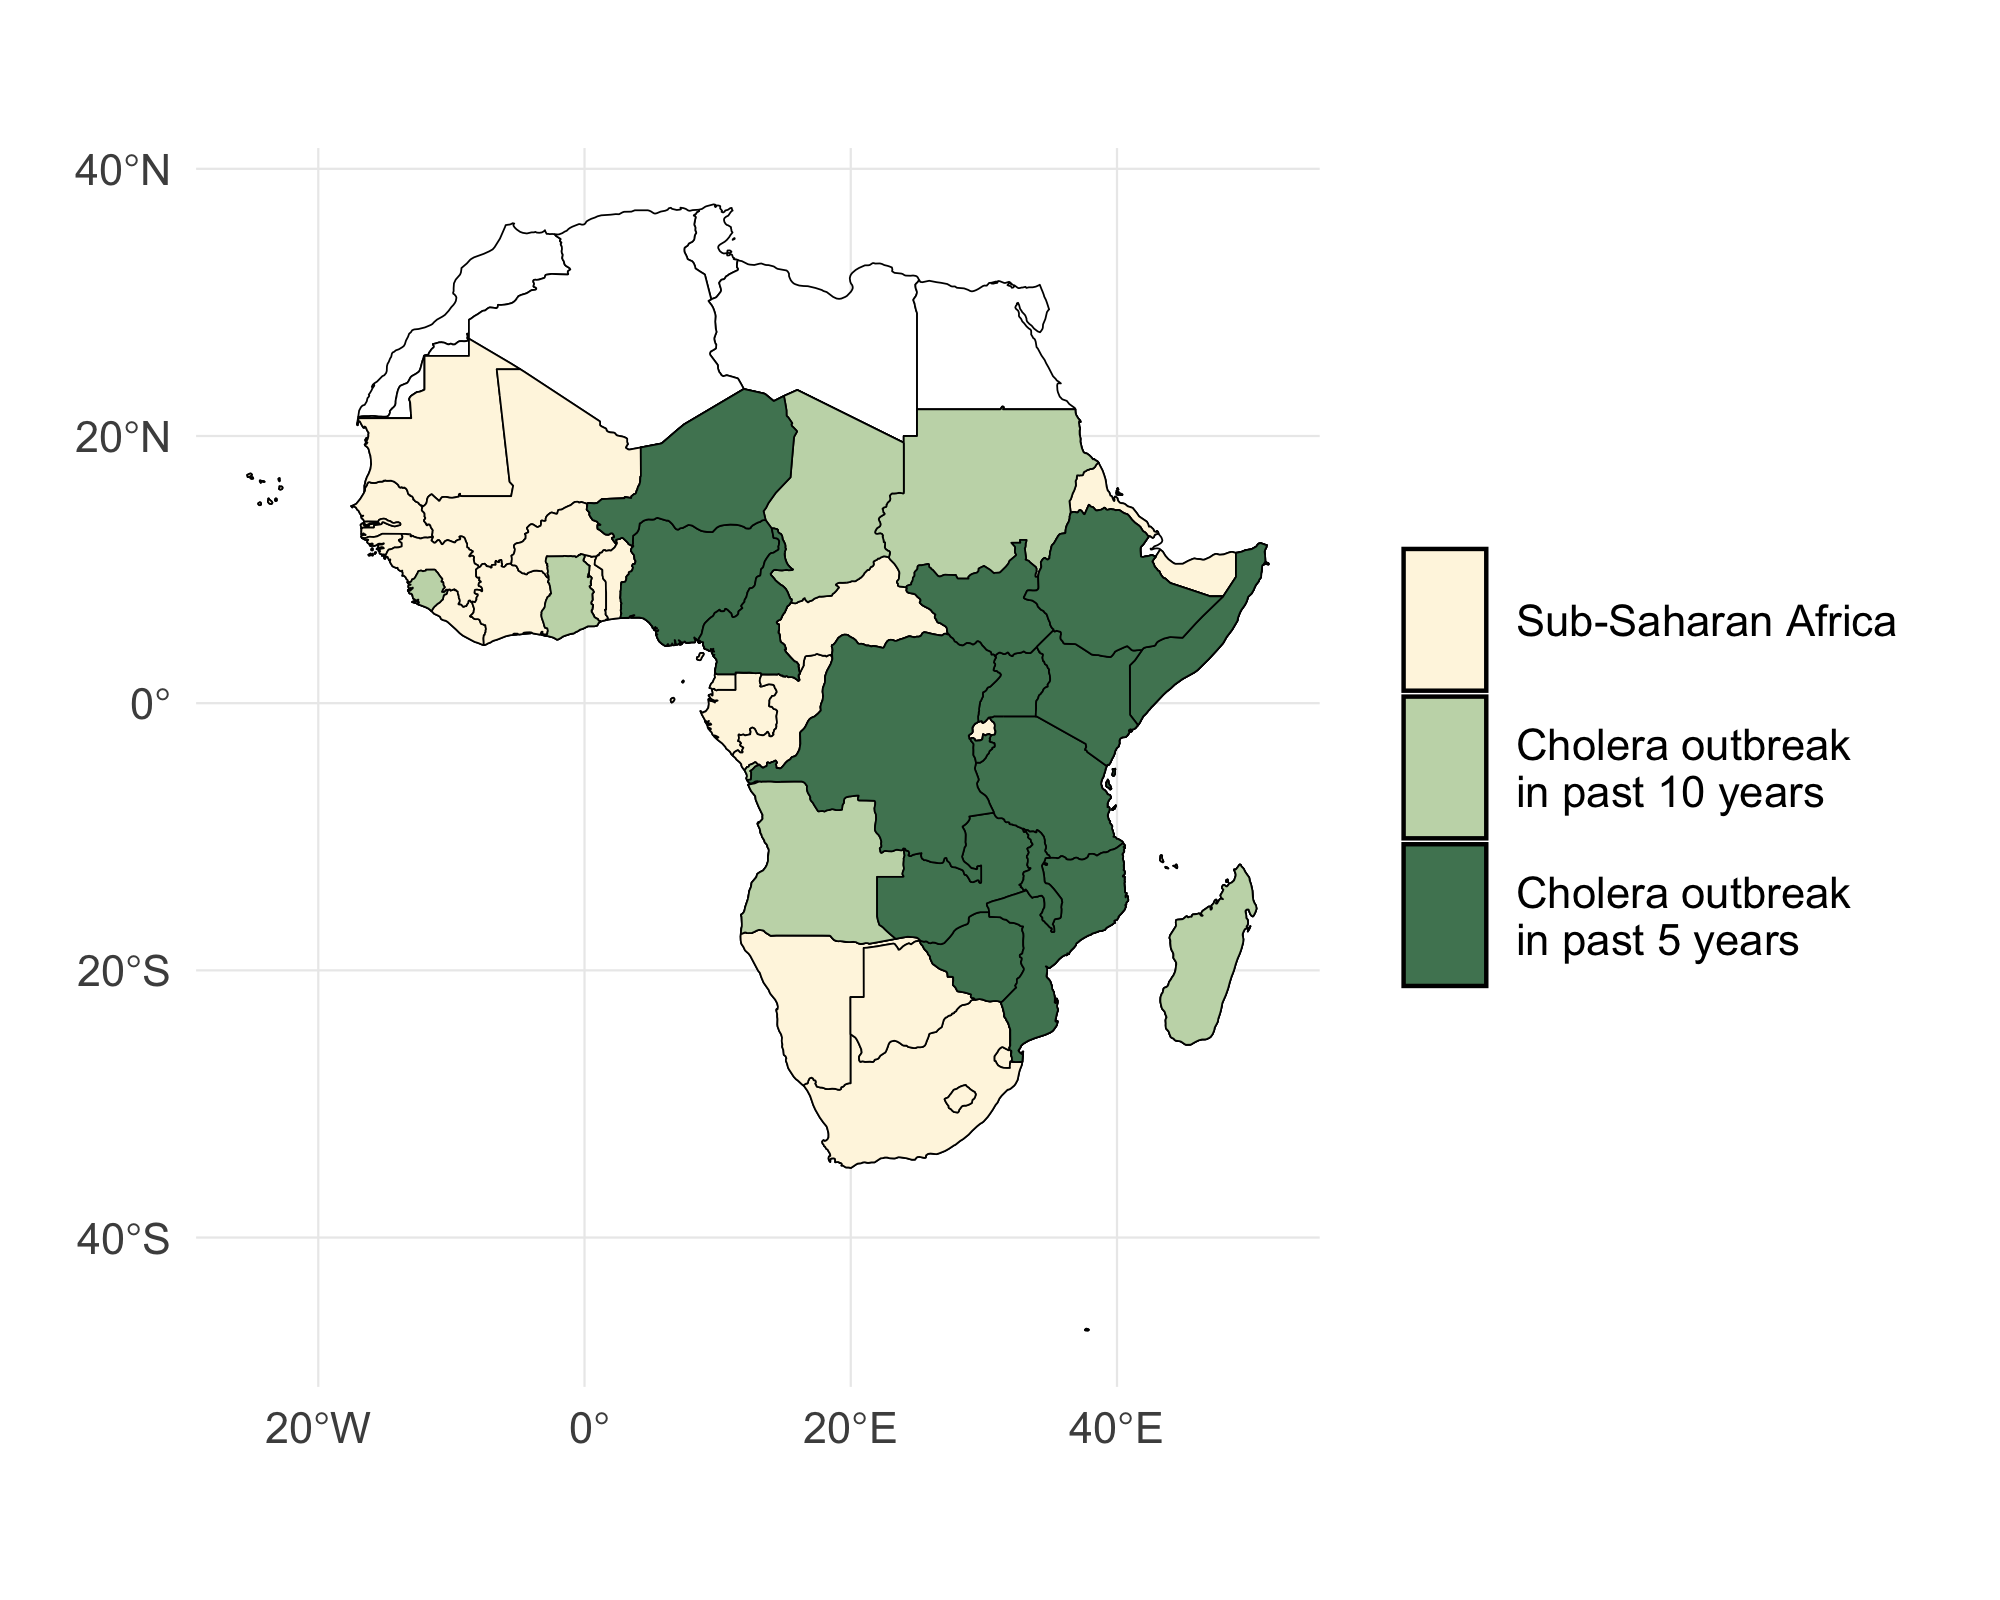
\includegraphics[width=1\linewidth]{figures/africa_map} 

}

\caption{A map of Sub-Saharan Africa with countries that have experienced a cholera outbreak in the past 5 and 10 years highlighted in green.}\label{fig:map}
\end{figure}

\section{Transmission dynamics}\label{transmission-dynamics}

The model has a metapopulation structure with familiar compartments for Susceptible, Infected, and Recovered individuals with SIRS dynamics. The model also contains compartments for vaccinated individuals (V) and Water \& environment based transmission (W) which we refer to as SVIWRS.

\begin{figure}

{\centering 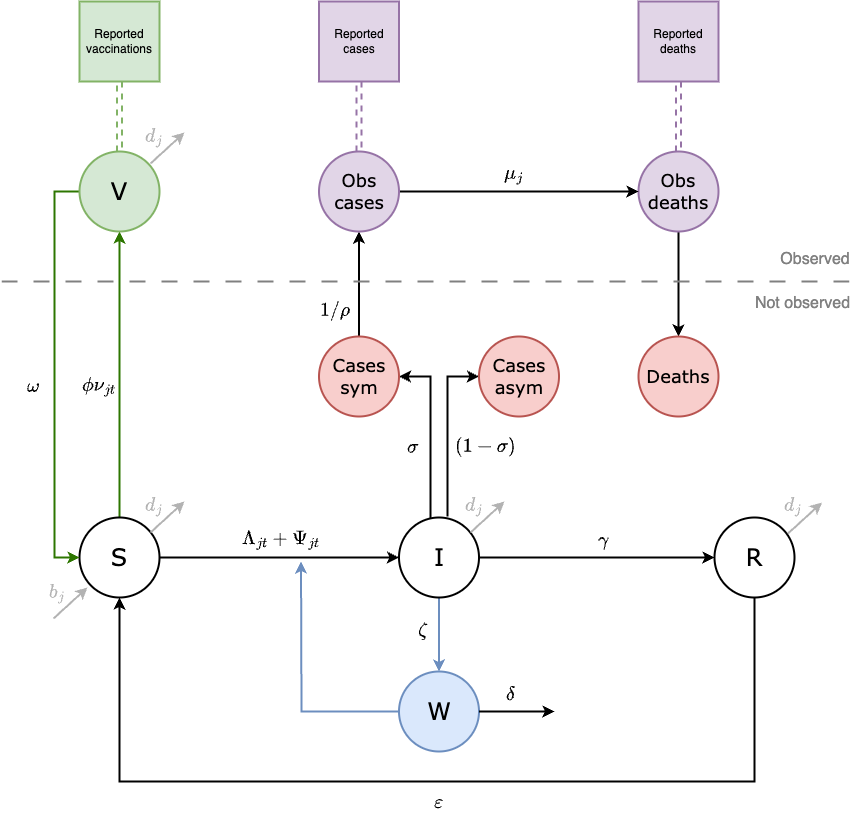
\includegraphics[width=0.95\linewidth]{diagrams/v_0_1.drawio} 

}

\caption{This diagram of the SVIWRS (Susceptible-Vaccinated-Infected-Water/environmental-Recovered-Susceptible) model shows model compartments as circles with rate parameters displayed. The primary data sources the model is fit to are shown as square nodes (Vaccination data, and reported cases and deaths).}\label{fig:diagram}
\end{figure}

The SVIWRS metapopulation model, shown in Figure \ref{fig:diagram}, is governed by the following difference equations:

\begin{equation}
\begin{aligned}
S_{j,t+1} &= b_j N_{jt} + S_{jt} - \phi \nu_{jt} S_{jt} + \omega V_{jt} - \Lambda_{j,t+1} - \Psi_{j,t+1} + \varepsilon R_{jt} - d_j S_{jt}\\[11pt]
V_{j,t+1} &= V_{jt} + \phi \nu_{jt} S_{jt} - \omega V_{jt} - d_j V_{jt}\\[11pt]
I_{j,t+1} &= I_{jt} + \Lambda_{j,t+1} + \Psi_{j,t+1} - \gamma I_{jt} - \mu \sigma I_{jt} - d_j I_{jt}\\[11pt]
W_{j,t+1} &= W_{jt} + \zeta I_{jt} - \delta_{jt} W_{jt}\\[11pt]
R_{j,t+1} &= R_{jt} + \gamma I_{jt} - \varepsilon R_{jt} - d_j R_{jt}\\[11pt]
\end{aligned}
\label{eq:system}
\end{equation}

For descriptions of all parameters in Equation \eqref{eq:system}, see Table (\ref{tab:params}). Transmission dynamics are driven by the two force of infection terms, \(\Lambda_{jt}\) and \(\Psi_{jt}\). The force of infection due to human-to-human (\(\Lambda_{jt}\)) is:

\begin{equation}
\begin{aligned}
\Lambda_{j,t+1} &= \frac{
\beta_{jt}^{\text{hum}} \Big(\big(S_{jt}(1-\tau_{j})\big)  \big(I_{jt}(1-\tau_{j}) + \sum_{\forall i \not= j} (\pi_{ij}\tau_iI_{it}) \big)\Big)^\alpha}{N_{jt}}.\\[11pt]
\end{aligned}
\label{eq:foi-human}
\end{equation}

Where \(\beta_{jt}^{\text{hum}}\) is the rate of human-to-human transmission. Movement within and among metapopulations is governed by \(\tau_i\), the probability of departing origin location \(i\), and \(\pi_{ij}\) is the relative probability of travel from origin \(i\) to destination \(j\) (see section on \hyperref[spatial-dynamics]{spatial dynamics}). To include environmental effects, the force of infection due to environment-to-human transmission (\(\Psi_{jt}\)) is defined as:

\begin{equation}
\begin{aligned}
\Psi_{j,t+1} &= \frac{\beta_{jt}^{\text{env}} \big(S_{jt}(1-\tau_{j})\big) (1-\theta_j) W_{jt}}{\kappa+W_{jt}},\\[11pt]
\end{aligned}
\label{eq:foi-environment}
\end{equation}

where \(\beta_{jt}^{\text{env}}\) is the rate of environment-to-human transmission and \(\theta_j\) is the proportion of the population at location \(j\) that at least basic access to Water, Sanitation, and Hygiene (WASH). The environmental compartment of the model is also scaled by the concentration (cells per mL) of \emph{V. cholerae} that is required for a 50\% probability of infection \href{https://www.ncbi.nlm.nih.gov/pmc/articles/PMC3926264/}{Fung 2014}. See the section on \hyperref[environmental-transmission]{environmental transmission} below for more on the water/environment compartment and climatic drivers of transmission.

Note that all model processes are stochastic. Transition rates are converted to probabilities with the commonly used formula \(p(t) = 1-e^{-rt}\) (see Ross 2007), and then integer quantities are moved between model compartments at each time step according to a binomial process like the example below for the recovery of infected individuals (\(\gamma I_{jt}\)):

\begin{equation}
\frac{\partial R}{\partial t} \sim \text{Binom}(I_{jt}, 1-\exp(-\gamma))
\label{eq:stoch}
\end{equation}

\section{Seasonality}\label{seasonality}

Cholera transmission is seasonal and is typically associated with the rainy season, so both transmission rate terms \(\beta_{jt}^{\text{*}}\) are temporally forced. For human-to-human transmission we used a truncated sine-cosine form of the \href{https://en.wikipedia.org/wiki/Fourier_series}{Fourier series} with two harmonic features which has the flexibility to capture seasonal transmission dynamics driven by extended rainy seasons and/or biannual trends:

\begin{equation}
\beta_{jt}^{\text{hum}} = \beta_{j0}^{\text{hum}} + a_1 \cos\left(\frac{2\pi t}{p}\right) + b_1 \sin\left(\frac{2\pi t}{p}\right) + a_2 \cos\left(\frac{4\pi t}{p}\right) + b_2 \sin\left(\frac{4\pi t}{p}\right)
\label{eq:beta1}
\end{equation}

Where, \(\beta_{j0}^{\text{hum}}\) is the mean human-to-human transmission rate at location \(j\) over all time steps. Seasonal dynamics are determined by the parameters \(a_1\), \(b_1\) and \(a_2\), \(b_2\) which gives the amplitude of the first and second waves respectively. The periodic cycle \(p\) is 52, so the function controls the temporal variation in \(\beta_{jt}^{\text{hum}}\) over the 52 weeks of the year.

\begin{figure}

{\centering 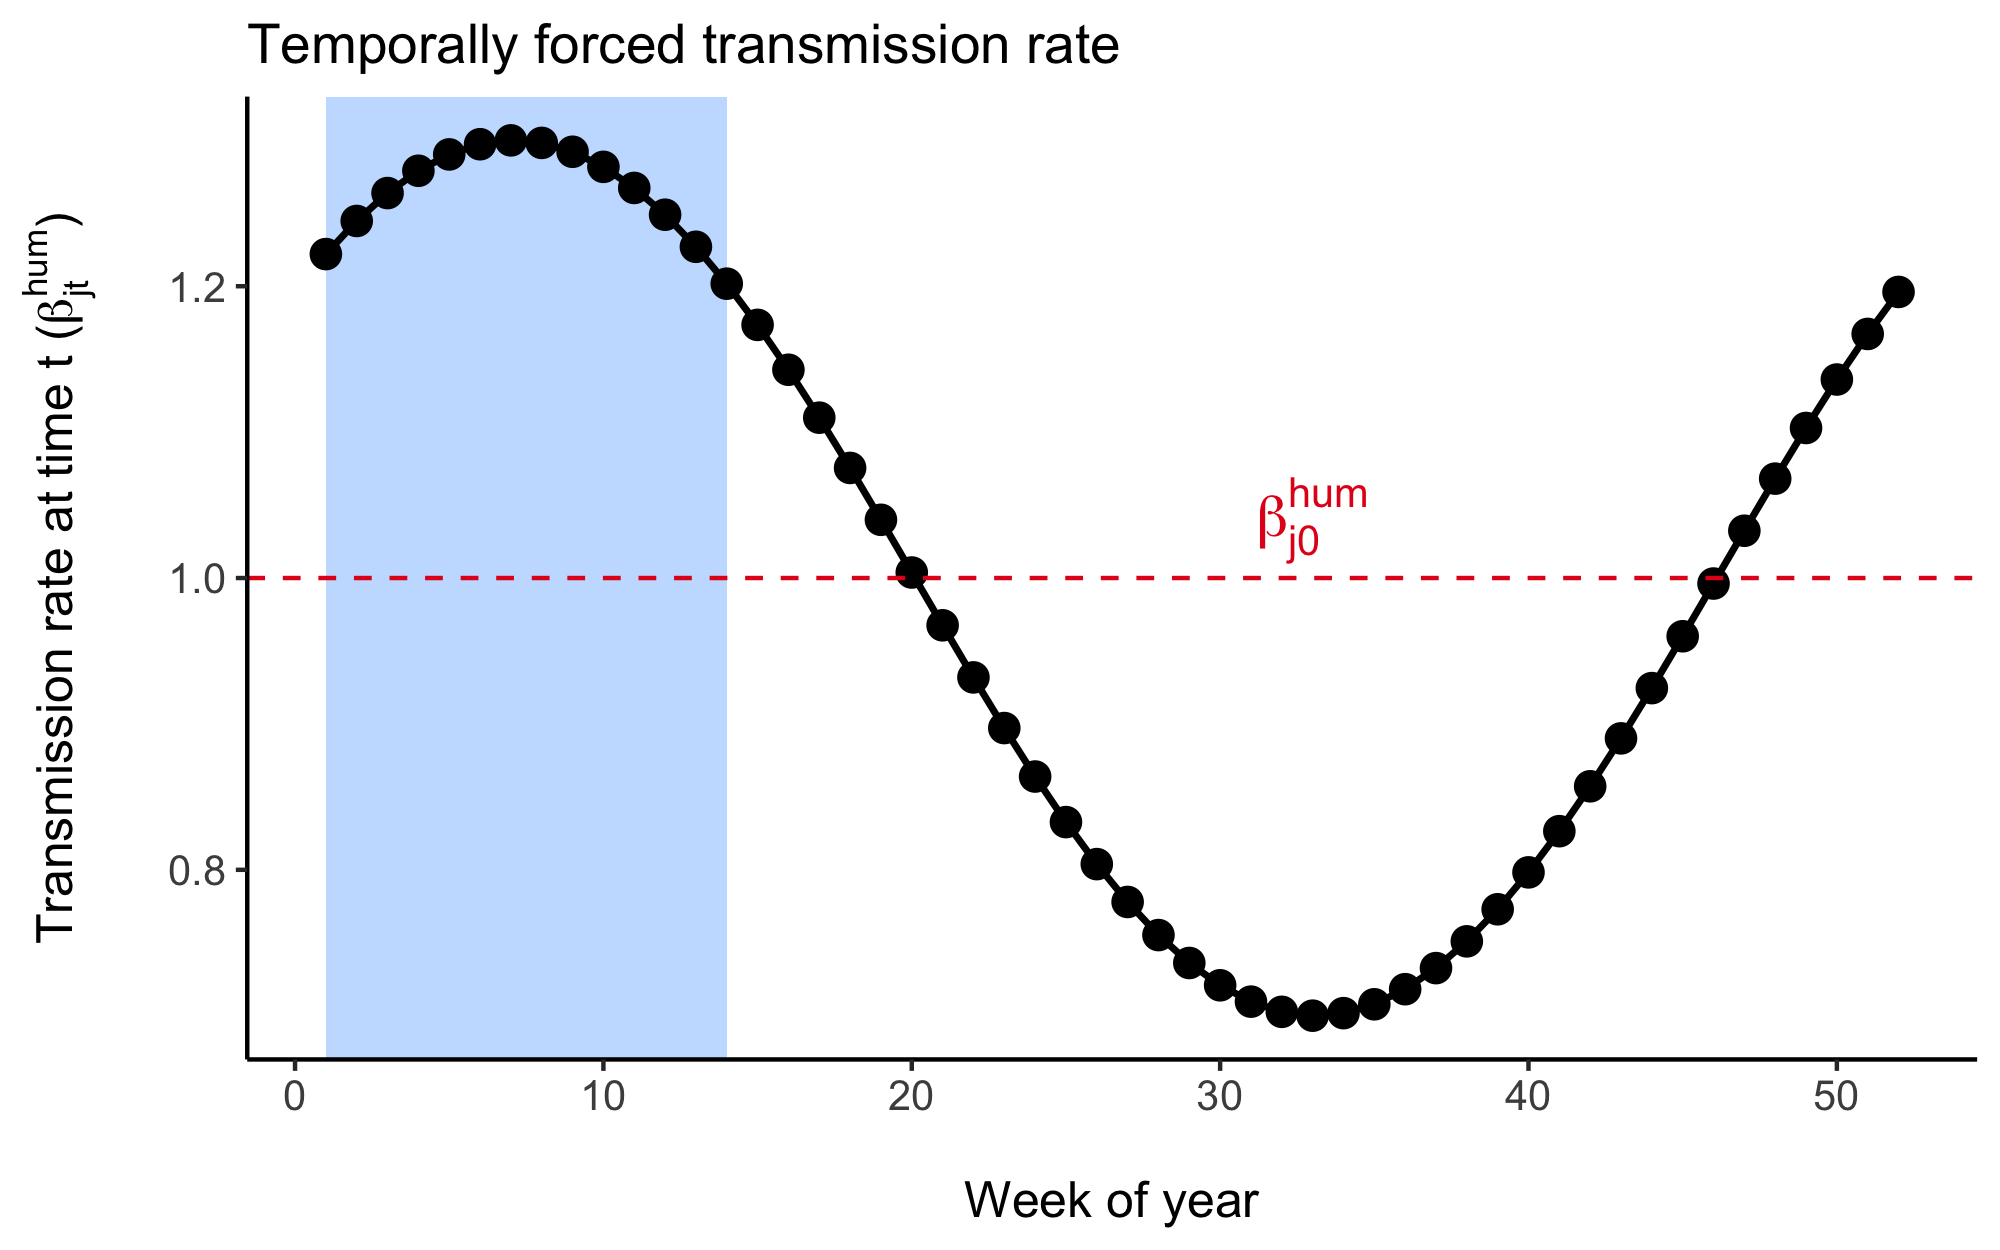
\includegraphics[width=0.85\linewidth]{figures/seasonal_transmission_concept} 

}

\caption{An example of the temporal distribution of the human-to-human transmission rate across each of the 52 weeks of the year given by the cosine wave function. The wave function is fitted to each country and is designed to align with the rainy season as indicated by the shaded region in this figure.}\label{fig:seasonal-concept}
\end{figure}

We estimated the parameters in the Fourier series (\(a_1\), \(b_1\), \(a_2\), \(b_2\)) using the \href{https://en.wikipedia.org/wiki/Levenberg\%E2\%80\%93Marquardt_algorithm}{Levenberg--Marquardt} algorithm in the \href{https://rdrr.io/cran/minpack.lm/}{\texttt{minpack.lm}} R library. Given the lack of reported cholera case data for many countries in SSA and the association between cholera transmission and the rainy season, we leveraged seasonal precipitation data to help fit the Fourier wave function to all countries. We first gathered weekly precipitation values from 1994 to 2024 for 30 uniformly distributed points within each country from the \href{https://open-meteo.com/en/docs/historical-weather-api}{Open-Meteo Historical Weather Data API}. Then we fit the Fourier series to the weekly precipitation data and used these parameters as the starting values when fitting the model to the more sparse cholera case data.

\begin{figure}

{\centering 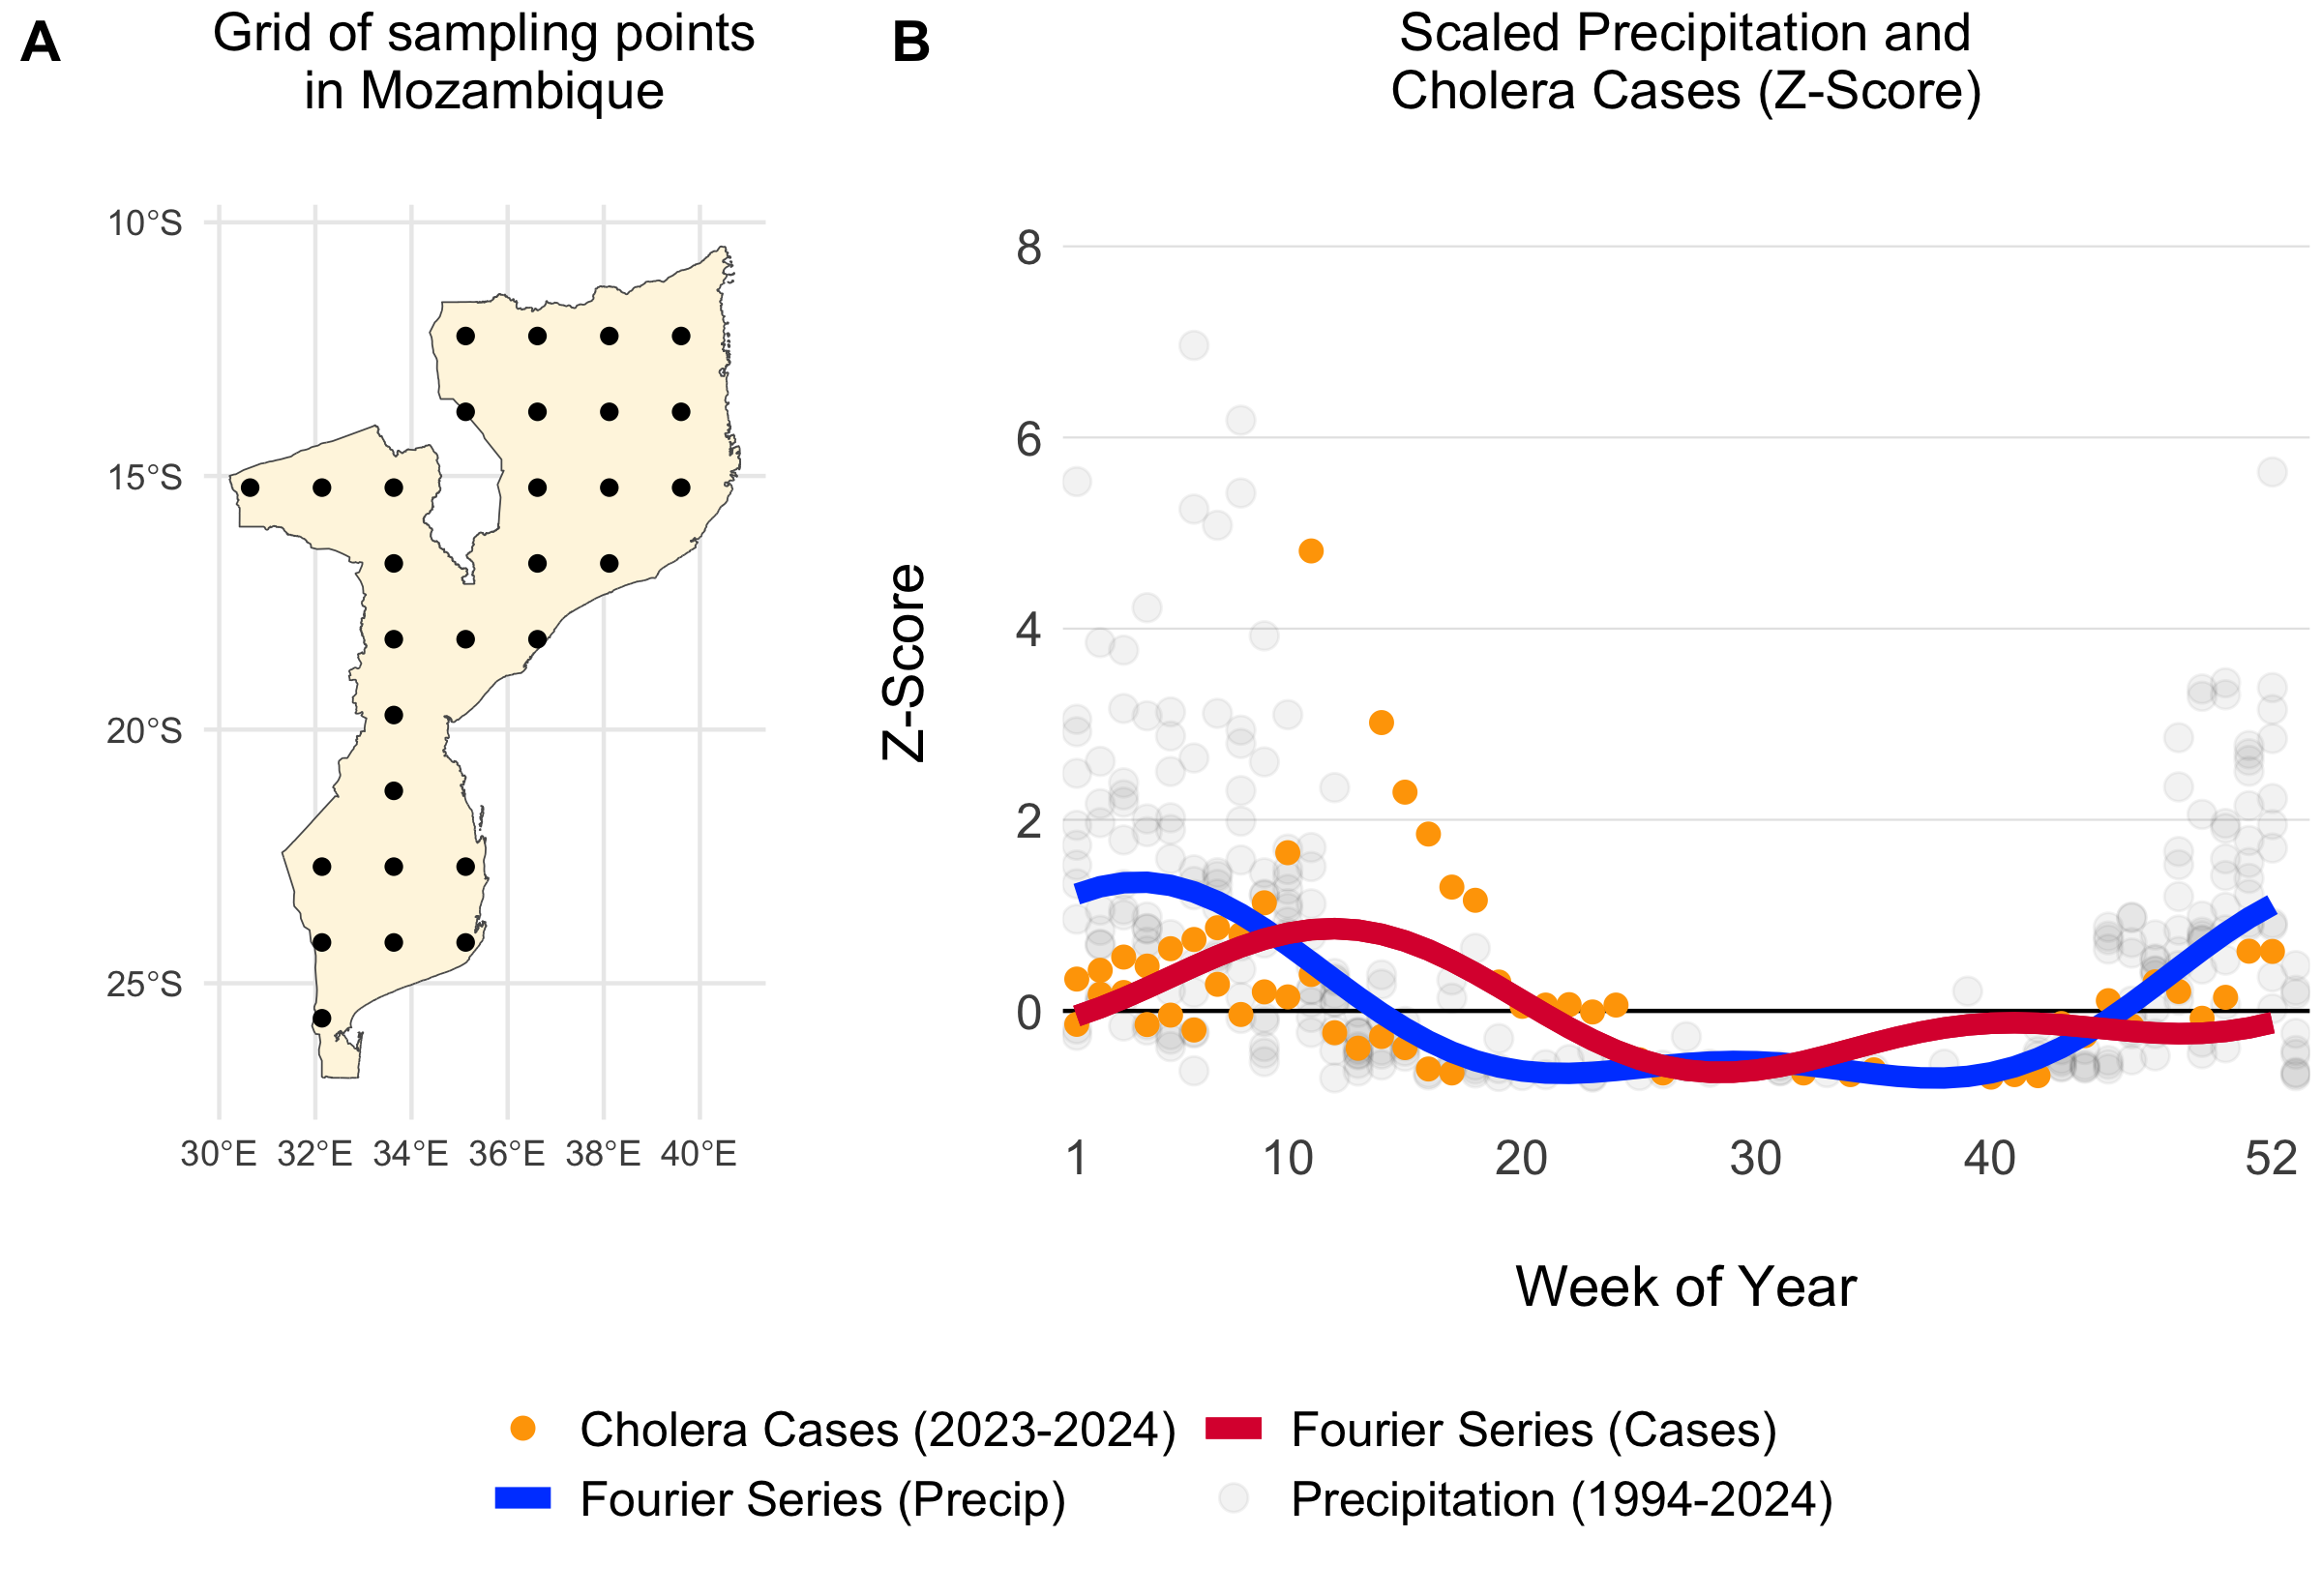
\includegraphics[width=1\linewidth]{figures/seasonal_transmission_example_MOZ} 

}

\caption{Example of a grid of 30 uniformly distributed points within Mozambique (A). The scatterplot shows weekly summed precipitation values at those 30 grid points and cholera cases plotted on the same scale of the Z-Score which shows the variance around the mean in terms of the standard deviation. Fitted Fourier series fucntions are shown as blue (fit precipitation data) and red (fit to cholera case data) lines.}\label{fig:seasonal-example}
\end{figure}

For countries with no reported case data, we inferred seasonal dynamics using the fitted wave function of a neighboring country with available case data. The selected neighbor was chosen from the same cluster of countries (grouped hierarchically into four clusters based on precipitation seasonality using \href{https://en.wikipedia.org/wiki/Ward\%27s_method}{Ward's method}; see Figure \ref{fig:seasonal-cluster}) that had the highest correlation in seasonal precipitation with the country lacking case data. In the rare event that no country with reported case data was found within the same seasonal cluster, we expanded the search to the 10 nearest neighbors and continued expanding by adding the next nearest neighbor until a match was found.

\begin{figure}

{\centering 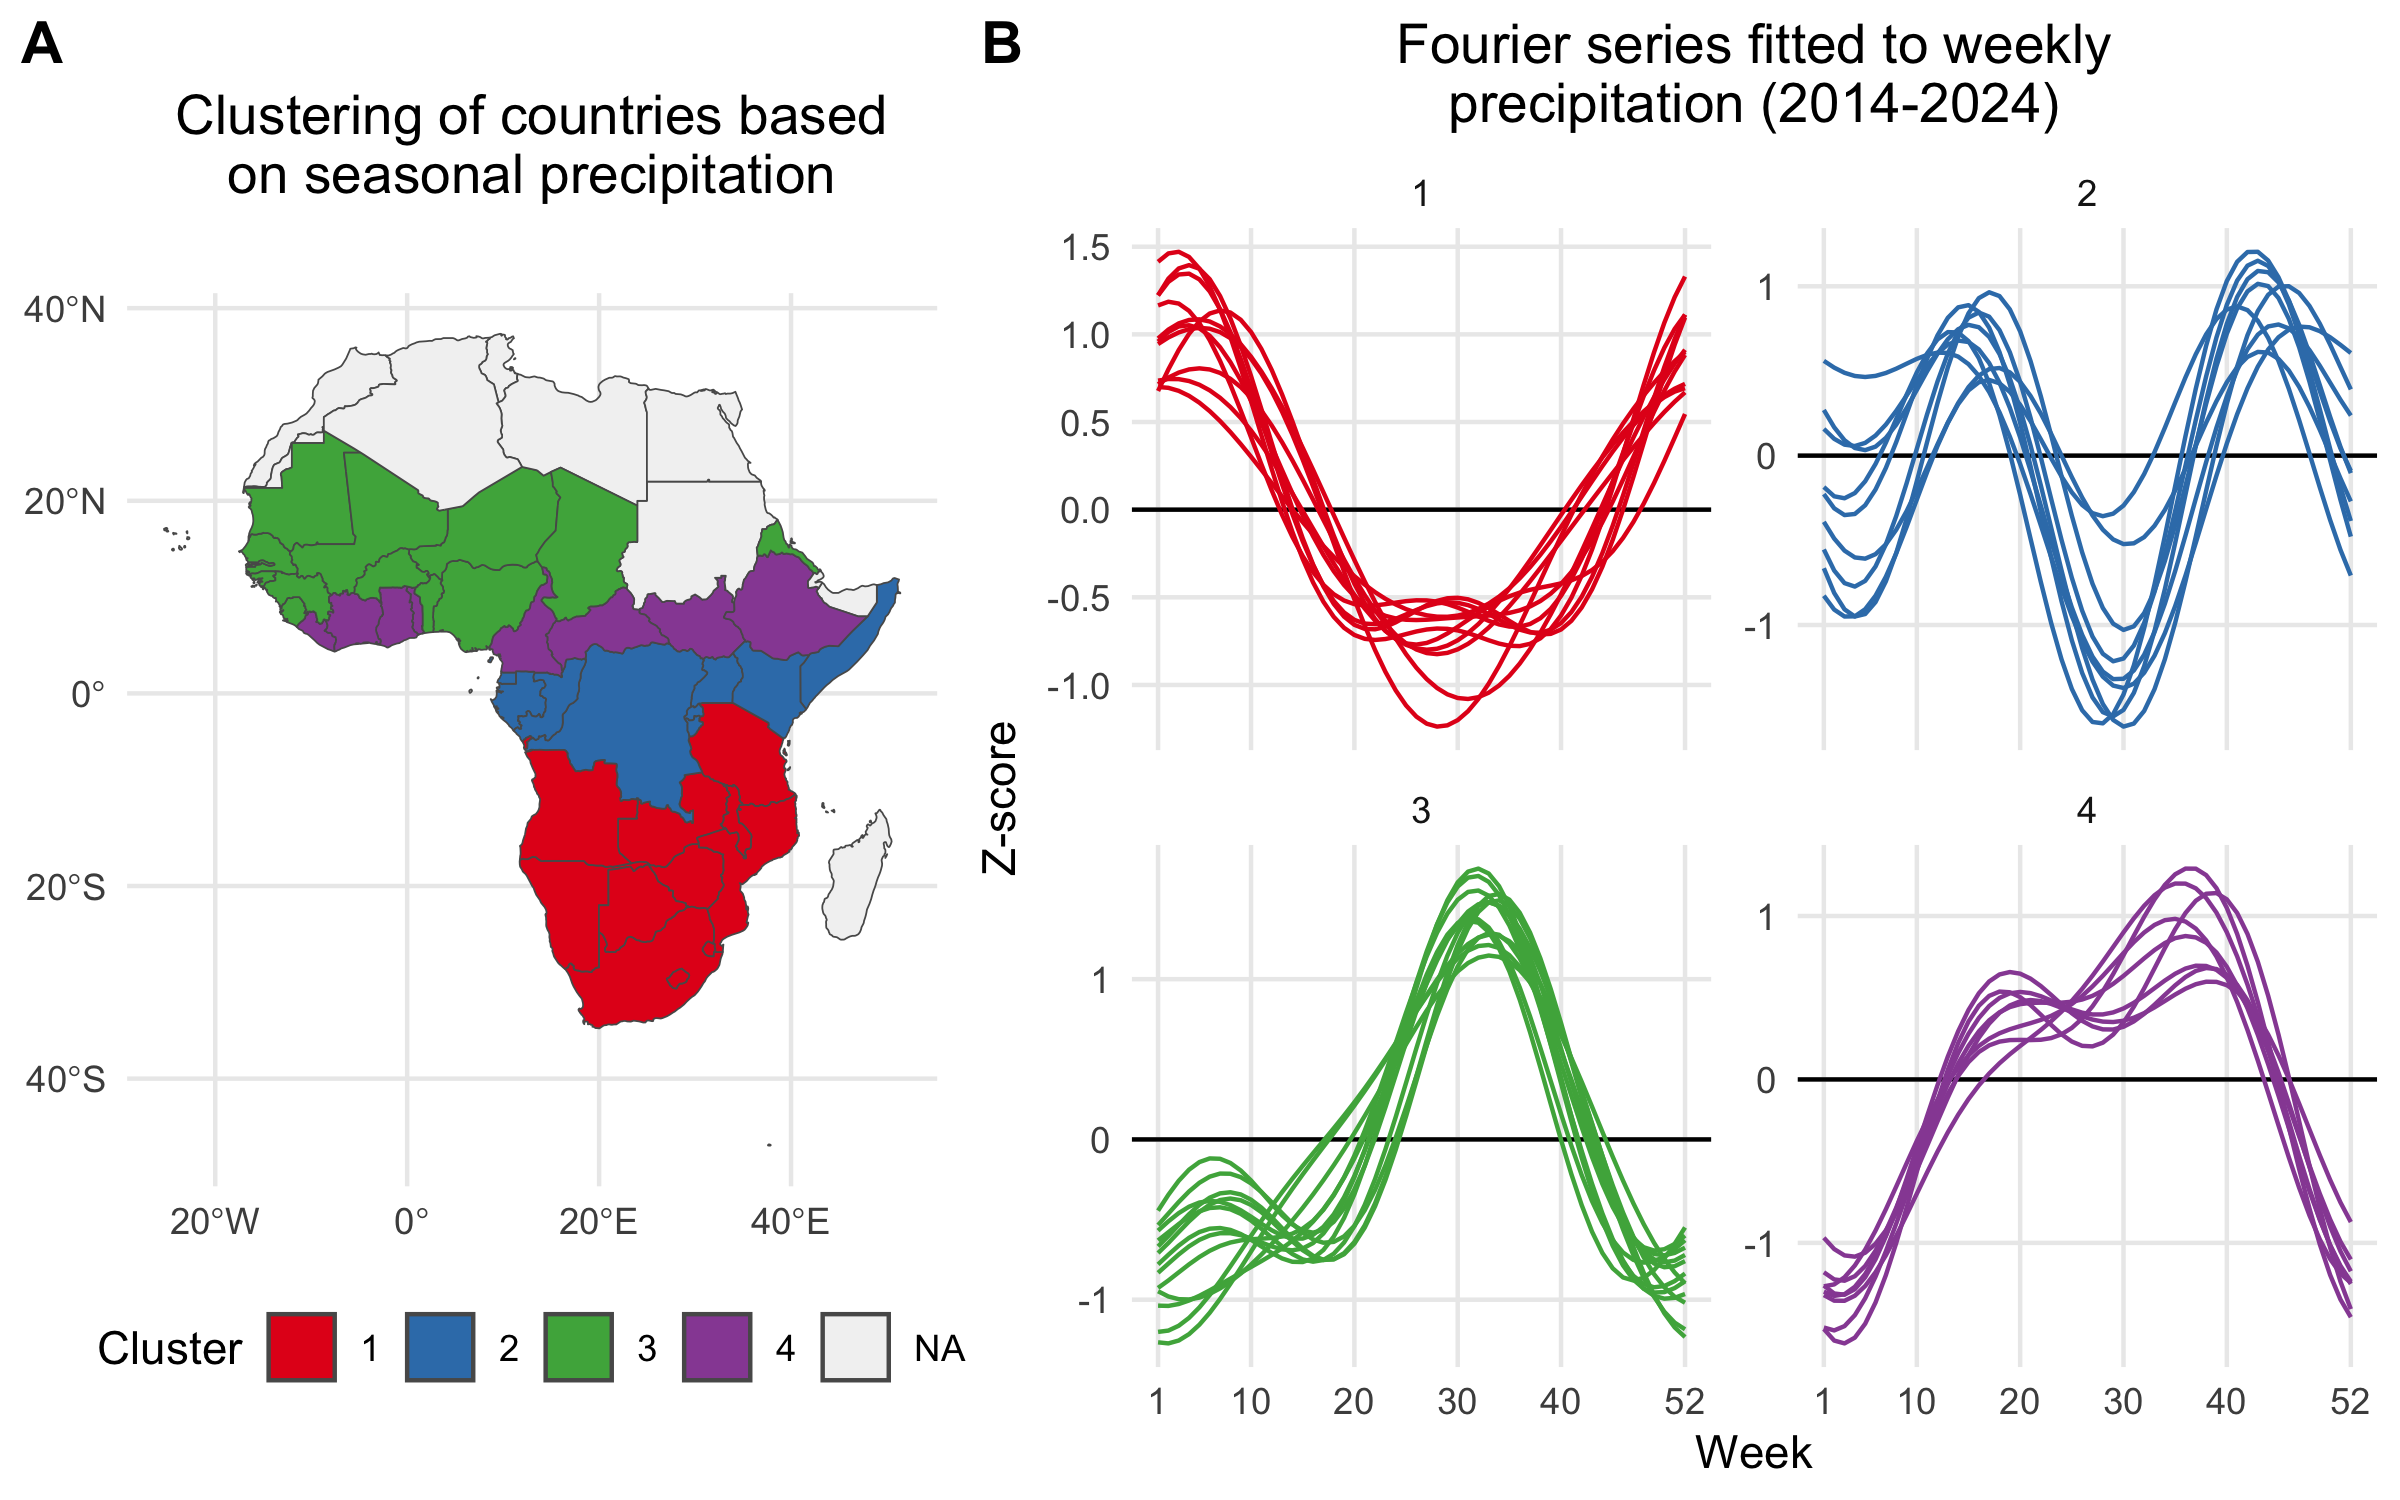
\includegraphics[width=1\linewidth]{figures/seasonal_precip_ward.D2_cluster} 

}

\caption{A) Map showing the clustering of African countries based on their seasonal precipitation patterns (2014-2024). Countries are colored according to their cluster assignments, identified using hierarchical clustering. B) Fourier series fitted to weekly precipitation for each country. Each line plot shows the seasonal pattern for countries within a given cluster. Clusteres are used to infer the seasonal transmission dynamics for countries where there are no reported cholera cases.}\label{fig:seasonal-cluster}
\end{figure}

Using the model fitting methods described above, and the cluster-based approach for inferring the seasonal Fourier series pattern in countries without reported cholera cases, we modeled the seasonal dynamics for all 41 countries in the MOSAIC framework. These dynamics are visualized in Figure \ref{fig:seasonal-all}, with the corresponding Fourier model coefficients presented in Table \ref{tab:seasonal-table}.

\begin{figure}

{\centering 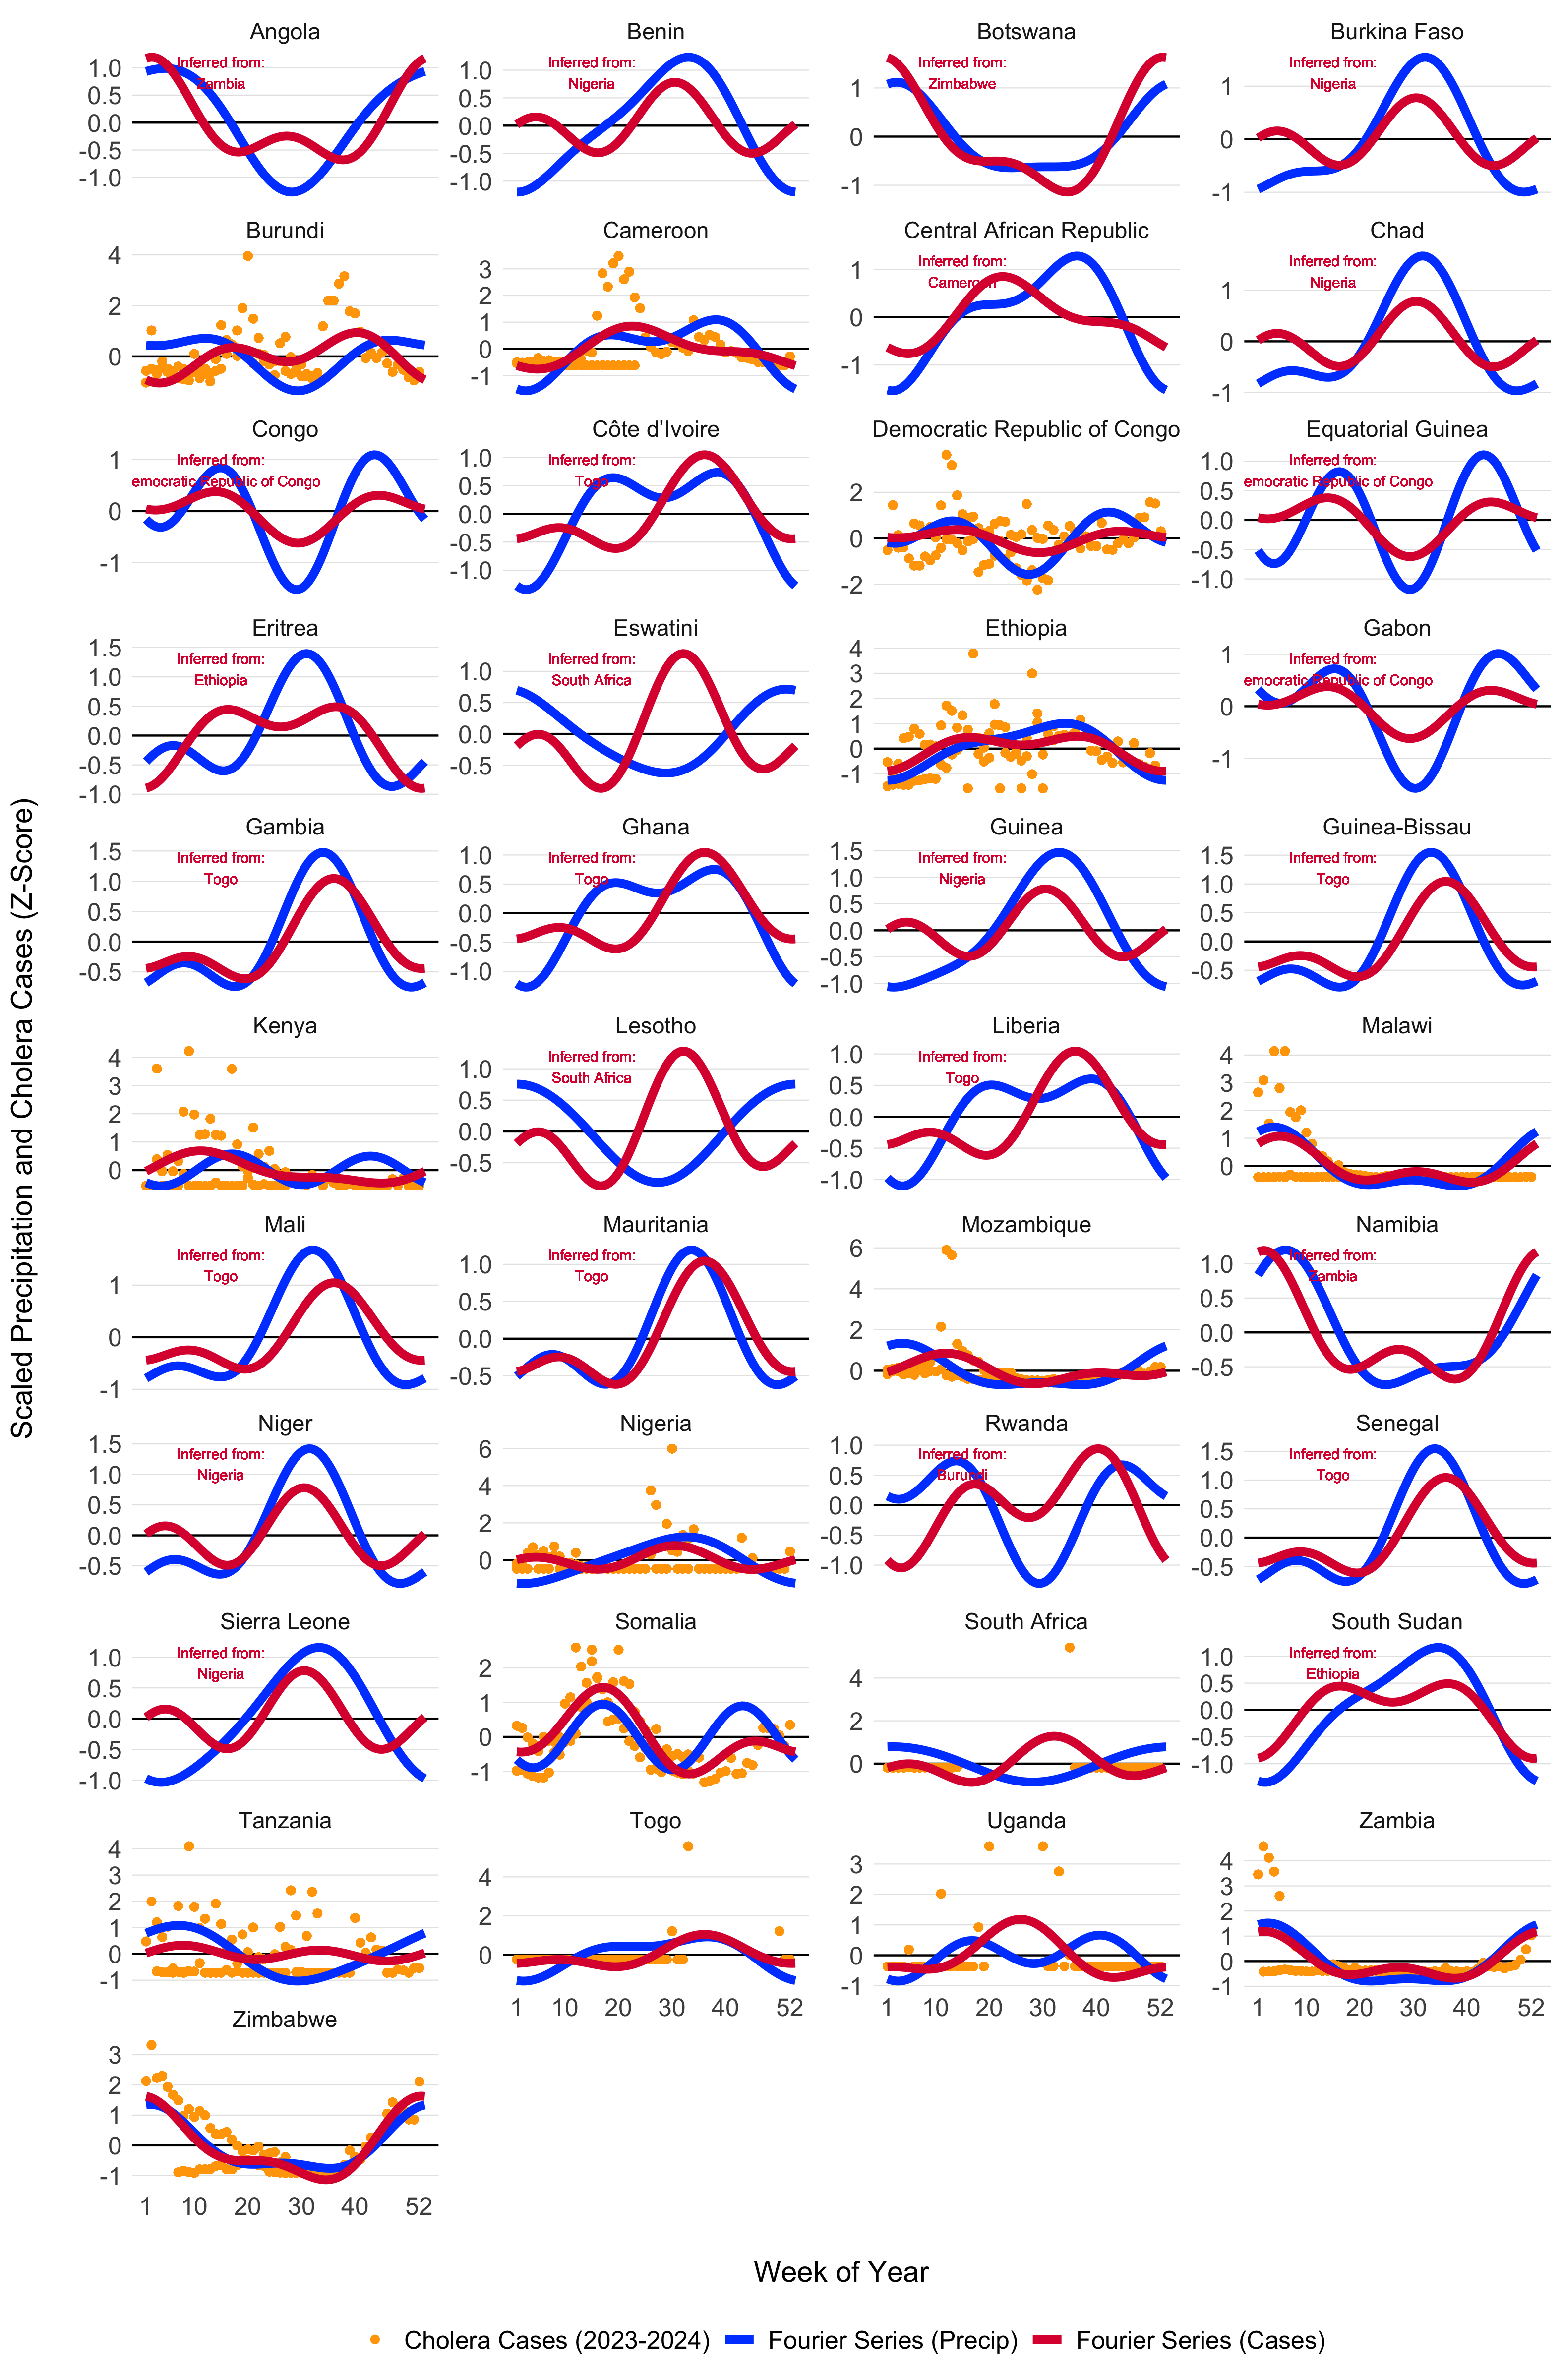
\includegraphics[width=1\linewidth]{figures/seasonal_transmission_all} 

}

\caption{Seasonal transmission patterns for all countries modeled in MOSAIC as modeled by the truncated Fourier series in Equation \\eqref{eq:beta1}. Blues lines give the Fourier series model fits for precipitation (1994-2024) and the red lines give models fits to reported cholera cases (2023-2024). For countries where reported case data were not available, the Fourier model was inferred by the nearest country with the most similar seasonal precipitation patterns as determined by the hierarchical clustering. Countries with inferred case data from neighboring locations are annotated in red. The X-axis represents the weeks of the year (1-52), while the Y-axis shows the Z-score of weekly precipitation and cholera cases.}\label{fig:seasonal-all}
\end{figure}

\begin{table}[!h]
\centering
\caption{\label{tab:seasonal-table}Estimated coefficients for the truncated Fourier model in Equation \\eqref{eq:beta1} fit to countries with reported cholera cases. Model fits are shown in Figure \\ref{fig:seasonal-all}.}
\centering
\fontsize{11.75}{13.75}\selectfont
\begin{tabular}[t]{l|l|l|l|l}
\hline
\multicolumn{1}{c|}{ } & \multicolumn{4}{c}{Fourier Coefficients} \\
\cline{2-5}
Country & $a_1$ & $a_2$ & $b_1$ & $b_2$\\
\hline
Burundi & -0.31 (-0.35 to -0.27) & -0.49 (-0.53 to -0.45) & -0.42 (-0.45 to -0.39) & -0.36 (-0.41 to -0.31)\\
\hline
Cameroon & -0.64 (-0.67 to -0.62) & 0.08 (0.04 to 0.11) & 0.01 (-0.04 to 0.06) & -0.28 (-0.31 to -0.26)\\
\hline
DRC & 0.28 (0.26 to 0.31) & -0.22 (-0.31 to -0.13) & 0.15 (0.08 to 0.23) & -0.2 (-0.28 to -0.13)\\
\hline
Ethiopia & -0.52 (-0.59 to -0.46) & -0.38 (-0.41 to -0.34) & -0.04 (-0.12 to 0.03) & -0.03 (-0.13 to 0.07)\\
\hline
Kenya & 0.03 (-0.02 to 0.07) & -0.16 (-0.19 to -0.12) & 0.5 (0.46 to 0.53) & 0.12 (0.09 to 0.15)\\
\hline
Malawi & 0.51 (0.47 to 0.54) & 0.16 (0.12 to 0.2) & 0.39 (0.36 to 0.43) & 0.4 (0.37 to 0.44)\\
\hline
Mozambique & 0.22 (0.19 to 0.26) & -0.36 (-0.39 to -0.33) & 0.48 (0.44 to 0.53) & 0.02 (-0.04 to 0.07)\\
\hline
Nigeria & -0.27 (-0.3 to -0.24) & 0.22 (0.15 to 0.29) & -0.16 (-0.2 to -0.11) & 0.42 (0.38 to 0.46)\\
\hline
Somalia & -0.16 (-0.2 to -0.12) & -0.24 (-0.3 to -0.17) & 0.84 (0.82 to 0.86) & -0.59 (-0.61 to -0.57)\\
\hline
South Africa & -0.41 (-0.62 to -0.19) & 0.13 (-0.07 to 0.33) & -0.54 (-0.67 to -0.41) & 0.63 (0.54 to 0.72)\\
\hline
Tanzania & 0.03 (0 to 0.06) & -0.06 (-0.12 to -0.01) & 0.09 (0.06 to 0.12) & 0.23 (0.2 to 0.26)\\
\hline
Togo & -0.17 (-0.45 to 0.12) & -0.28 (-0.43 to -0.13) & -0.63 (-0.72 to -0.54) & 0.28 (0.06 to 0.51)\\
\hline
Uganda & -0.79 (-0.9 to -0.69) & 0.39 (0.32 to 0.46) & 0.12 (-0.07 to 0.31) & 0.04 (-0.16 to 0.23)\\
\hline
Zambia & 0.69 (0.63 to 0.74) & 0.43 (0.39 to 0.46) & 0.23 (0.18 to 0.28) & 0.2 (0.14 to 0.26)\\
\hline
Zimbabwe & 1.12 (1.08 to 1.17) & 0.51 (0.48 to 0.53) & 0.3 (0.24 to 0.35) & -0.08 (-0.13 to -0.03)\\
\hline
\end{tabular}
\end{table}

\section{Environmental transmission}\label{environmental-transmission}

Environmental transmission is a critical factor in cholera spread and consists of several key components: the rate at which infected individuals shed \emph{V. cholerae} into the environment, the pathogen's survival rate in environmental conditions, and the overall suitability of the environment for sustaining the bacteria over time.

\subsection{Climate-driven transmission}\label{climate-driven-transmission}

To capture the impacts of climate-drivers on cholera transmission, we have included the parameter \(\psi_{jt}\), which represents the current state of environmental suitability with respect to: \emph{i}) the survival time of \emph{V. cholerae} in the environment and, \emph{ii}) the rate of environment-to-human transmission which contributes to the overall force of infection.

\begin{equation}
\beta_{jt}^{\text{env}} = \beta_{j0}^{\text{env}} \Bigg(1 + \frac{\psi_{jt}-\bar\psi_j}{\bar\psi_j} \Bigg) \quad \text{and} \quad \bar\psi_j = \frac{1}{T} \sum_{t=1}^{T} \psi_{jt}
\label{eq:beta2}
\end{equation}

This formulation effectively scales the base environmental transmission rate \(\beta_{jt}^{\text{env}}\) so that it varies over time according to the climatically driven model of suitability. Note that, unlike the the cosine wave function of \(\beta_{jt}^{\text{hum}}\), this temporal term can increase or decrease over time following multi-annual cycles.

Environmental suitability (\(\psi_{jt}\)) also impacts the survival rate of \emph{V. cholerae} in the environment (\(\delta_{jt}\)) with the form:

\begin{equation}
\delta_{jt} = \delta_{\text{min}} + \psi_{jt} \times (\delta_{\text{max}} - \delta_{\text{min}})
\label{eq:delta}
\end{equation}

which normalizes the variance of the suitability parameter to be bounded within the minimum (\(\delta_{\text{min}}\)) and maximum (\(\delta_{\text{max}}\)) survival times of \emph{V. cholerae}.

\begin{figure}

{\centering 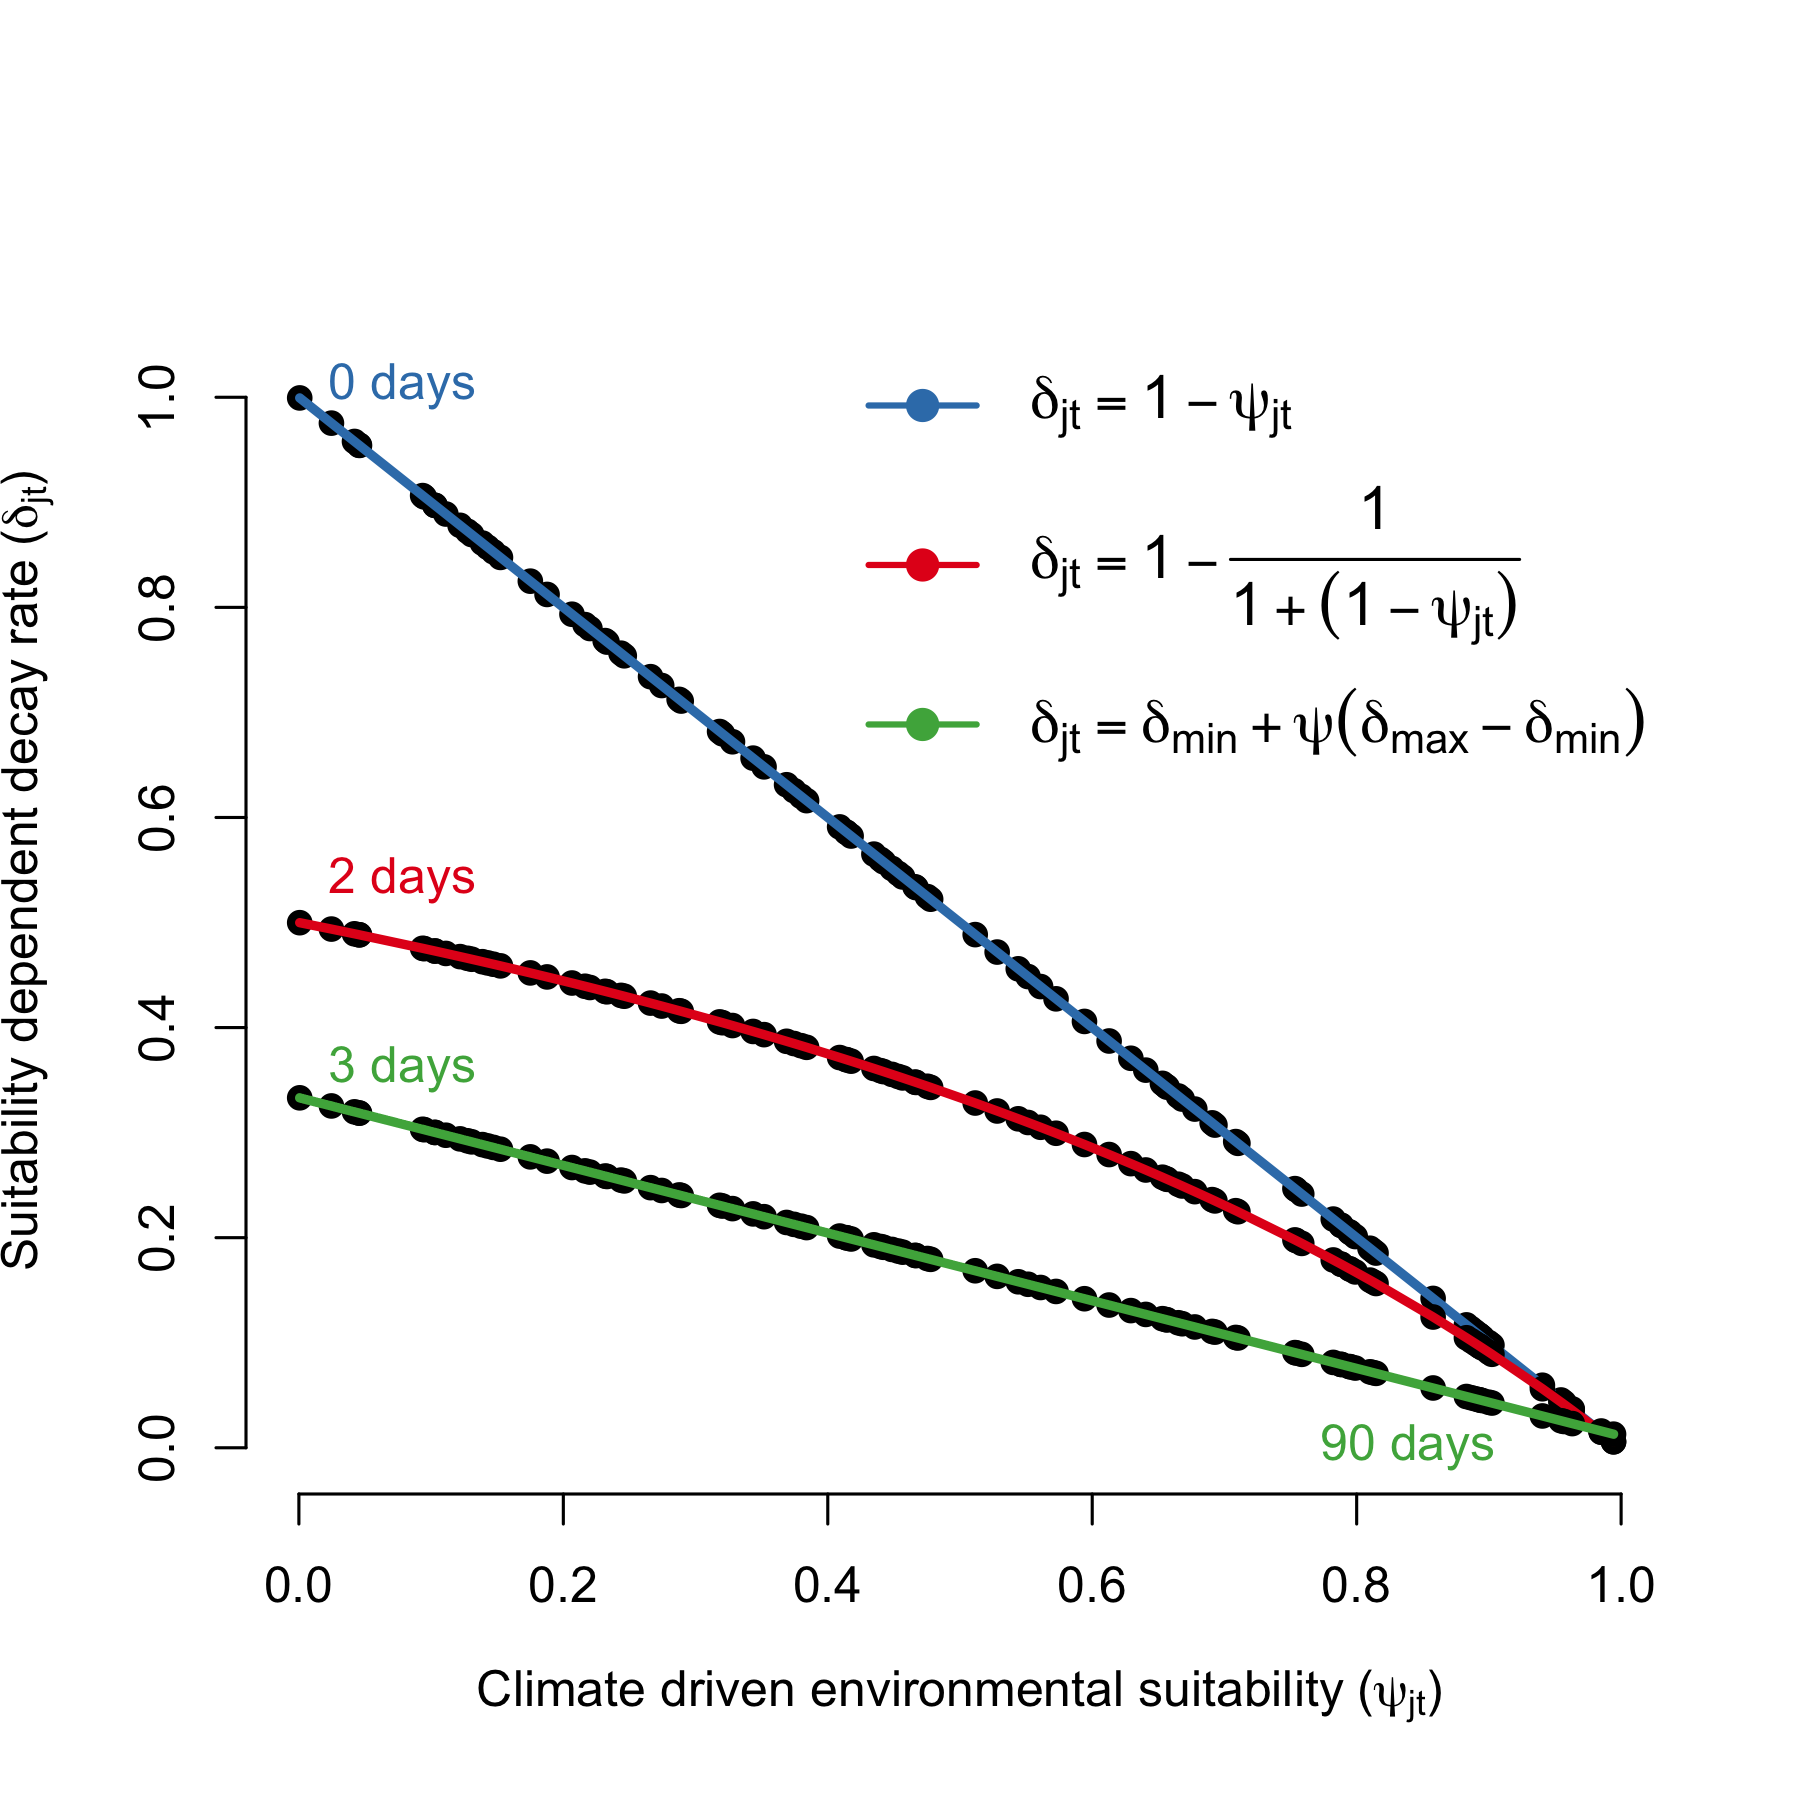
\includegraphics[width=0.8\linewidth]{figures/shedding_rate} 

}

\caption{Relationship between environmental suitability ($\psi_{jt}$) and the rate of *V. cholerae* decay in the environment ($\delta_j$). The green line shows the mildest penalty on *V. cholerae* survival, where survival in the environment is $1/\delta_{\text{min}}$ = 3 days when suitability = 0 and $1/\delta_{\text{max}}$ = 90 days when suitability = 1.}\label{fig:unnamed-chunk-2}
\end{figure}

\subsection{Modeling environmental suitability}\label{modeling-environmental-suitability}

\subsubsection{Environmental data}\label{environmental-data}

The mechanism for environment-to-human transmission (Equation \eqref{eq:beta2}) and rate of decay of \emph{V. cholerae} in the environment (Equation \eqref{eq:delta}) is driven by the parameter \(\psi_{jt}\), which we refer to as environmental suitability. The parameter \(\psi_{jt}\) is modeled as a time series for each location using a Long Short-Term Memory (LSTM) Recurrent Neural Network (RNN) model and a suite of 24 covariates which include 19 historical and forecasted climate variables under the \href{https://www.wdc-climate.de/ui/cmip6?input=CMIP6.HighResMIP.MRI.MRI-AGCM3-2-S.highresSST-present}{MRI-AGCM3-2-S} climate model. Covariates also include 4 large-scale climate drivers such as the Indian Ocean Dipole Mode Index (DMI), and the El Niño Southern Oscillation (ENSO) from 3 different Pacific Ocean regions. We also included a location specific variable giving the mean elevation for each country. See example time series of climate variables from one country (Mozambique) in Figure \ref{fig:climate-data-moz} and DMI and ENSO variables in Figure \ref{fig:climate-data-enso}. A list of all covariates and their sources can be seen in Table \ref{tab:climate-data-variables}.

Note that while the 19 climate variables offer forecasts up to 2030 and beyond, the forecasts of the DMI and ENSO variables are limited to 5 months into the future. So, environmental suitability model predictions are currently limited to a 5 month time horizon but future iterations may allow for longer forecasts. Additional data sources will be integrated into subsequent versions of the suitability model. For instance, flood and cyclone data will likely be incorporated later, though not in the initial version of the model.

\begin{figure}

{\centering 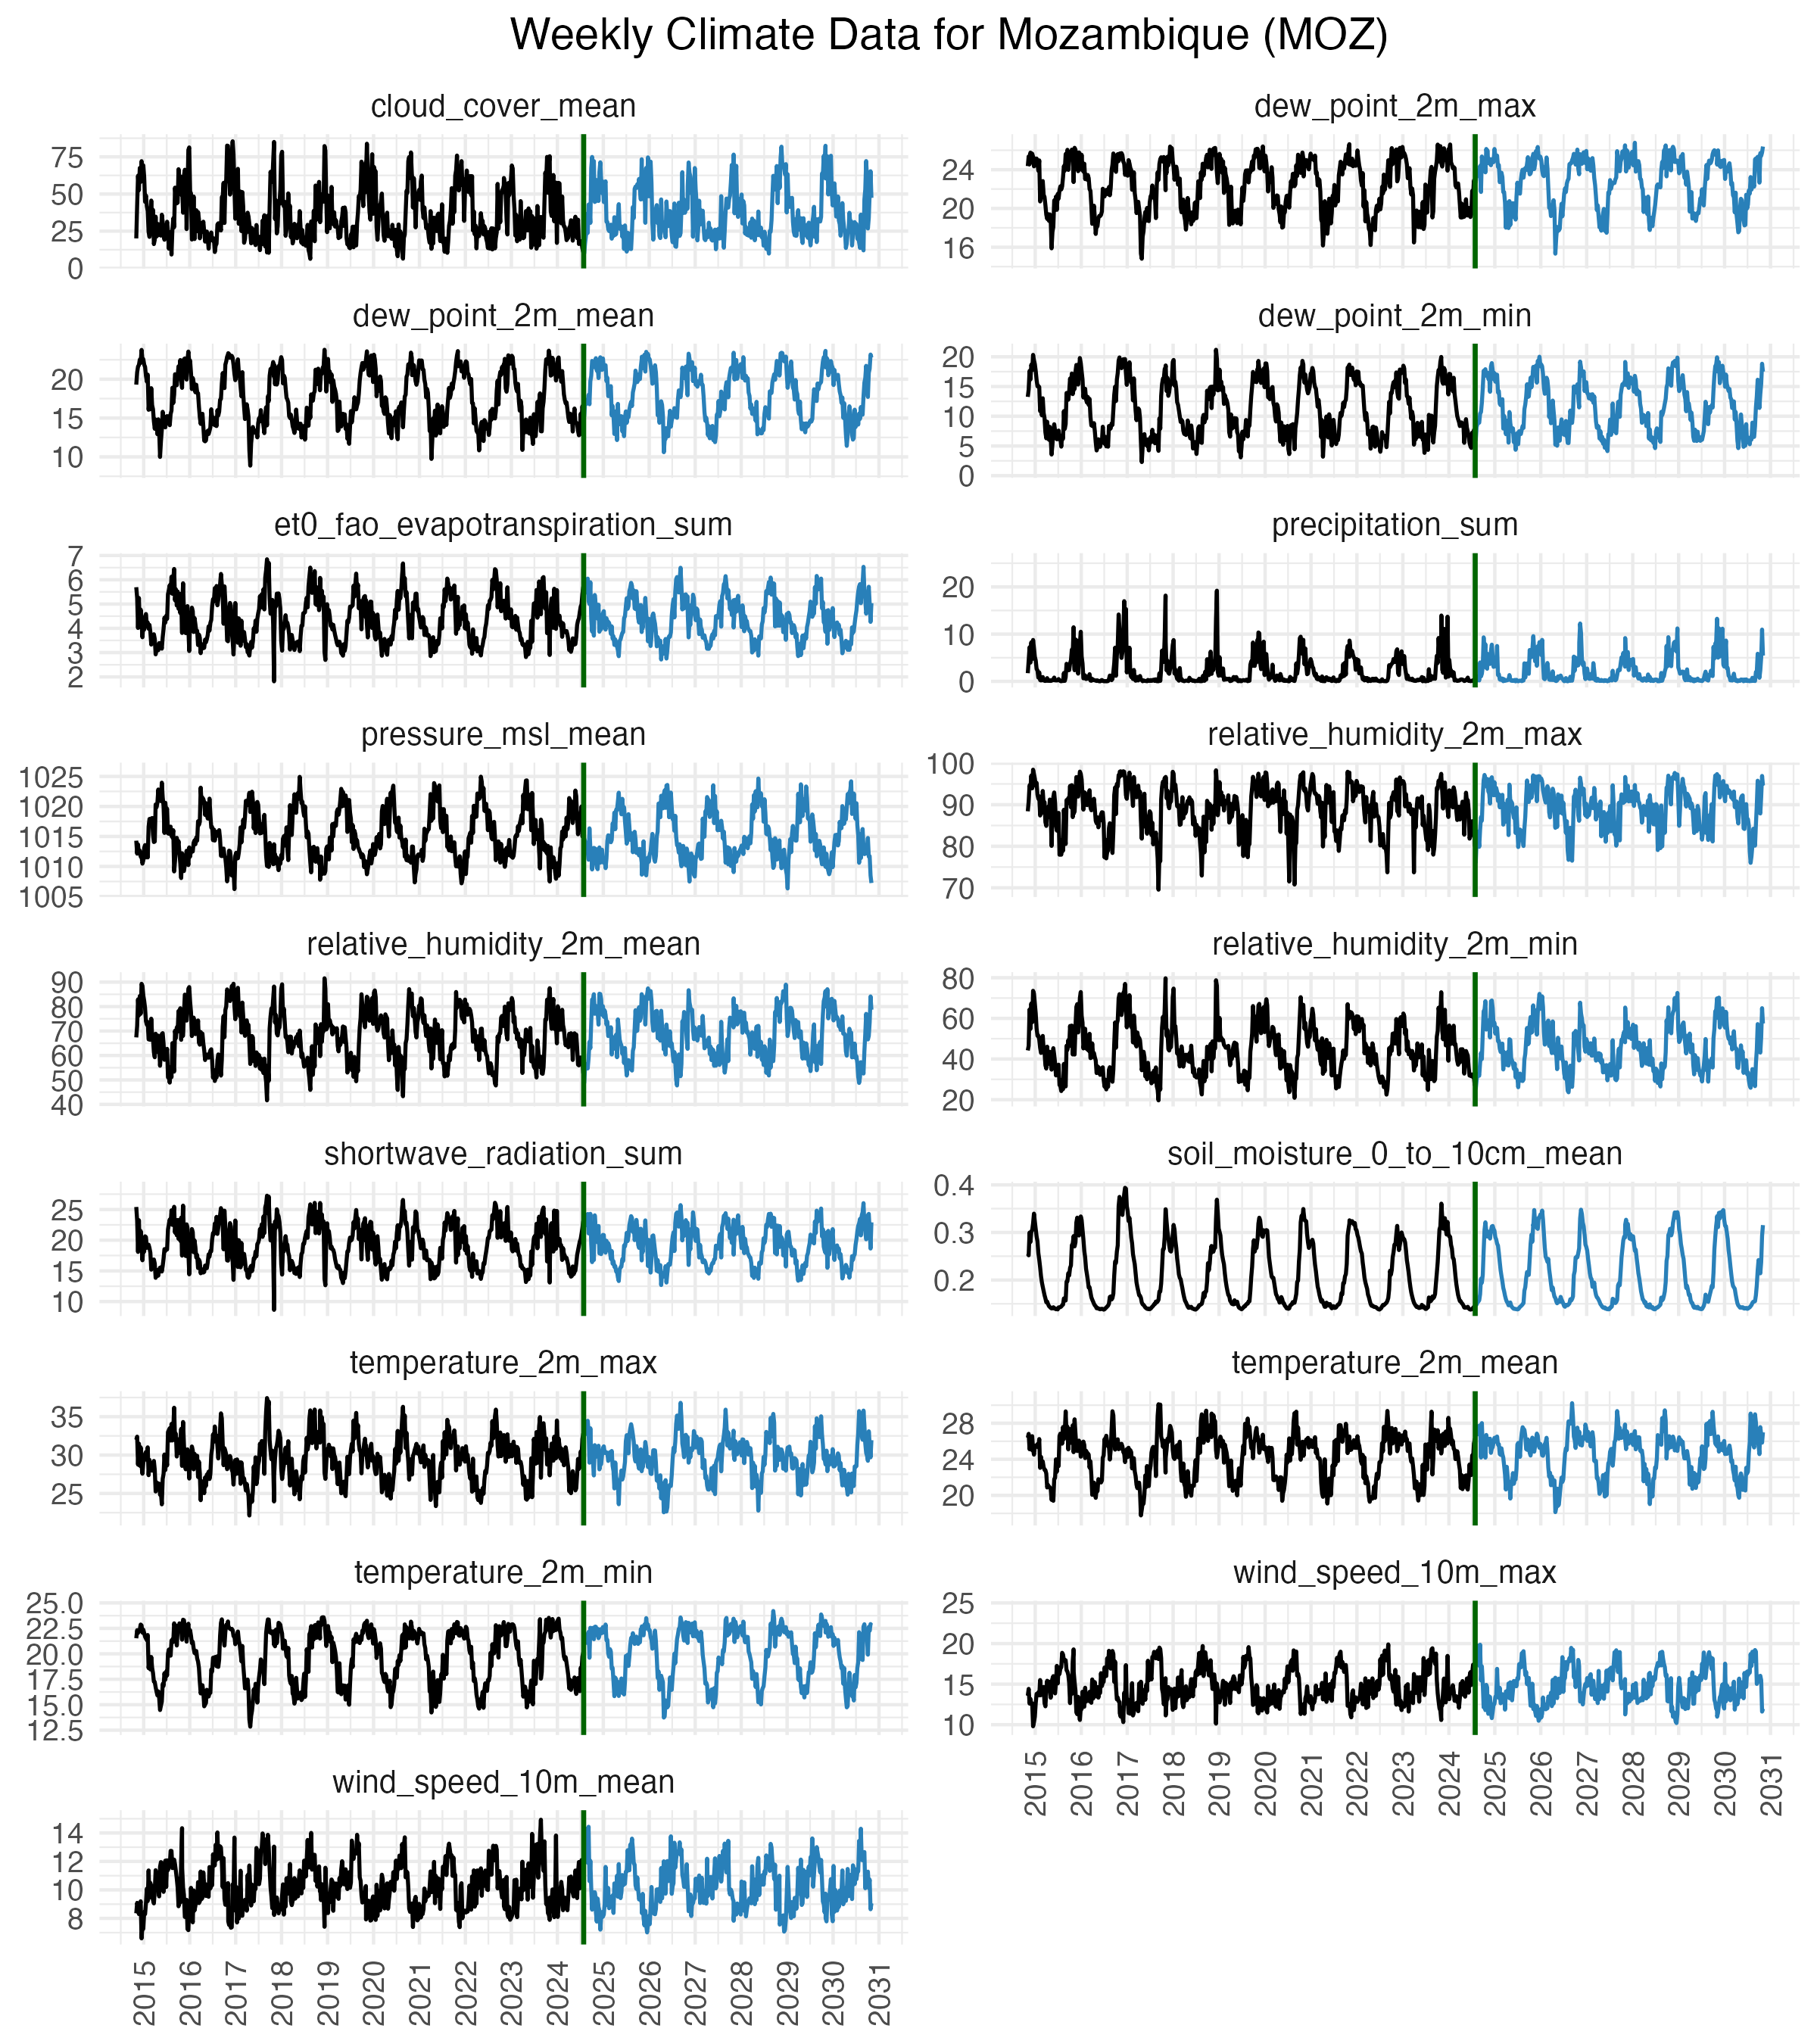
\includegraphics[width=1\linewidth]{figures/climate_data_MOZ_weekly} 

}

\caption{Climate data acquired from the OpenMeteo data API. Data were collected from 30 uniformly distributed points across each country and then aggregated to give weekly values of 17 climate variable from 1970 to 2030.}\label{fig:climate-data-moz}
\end{figure}

\begin{figure}

{\centering 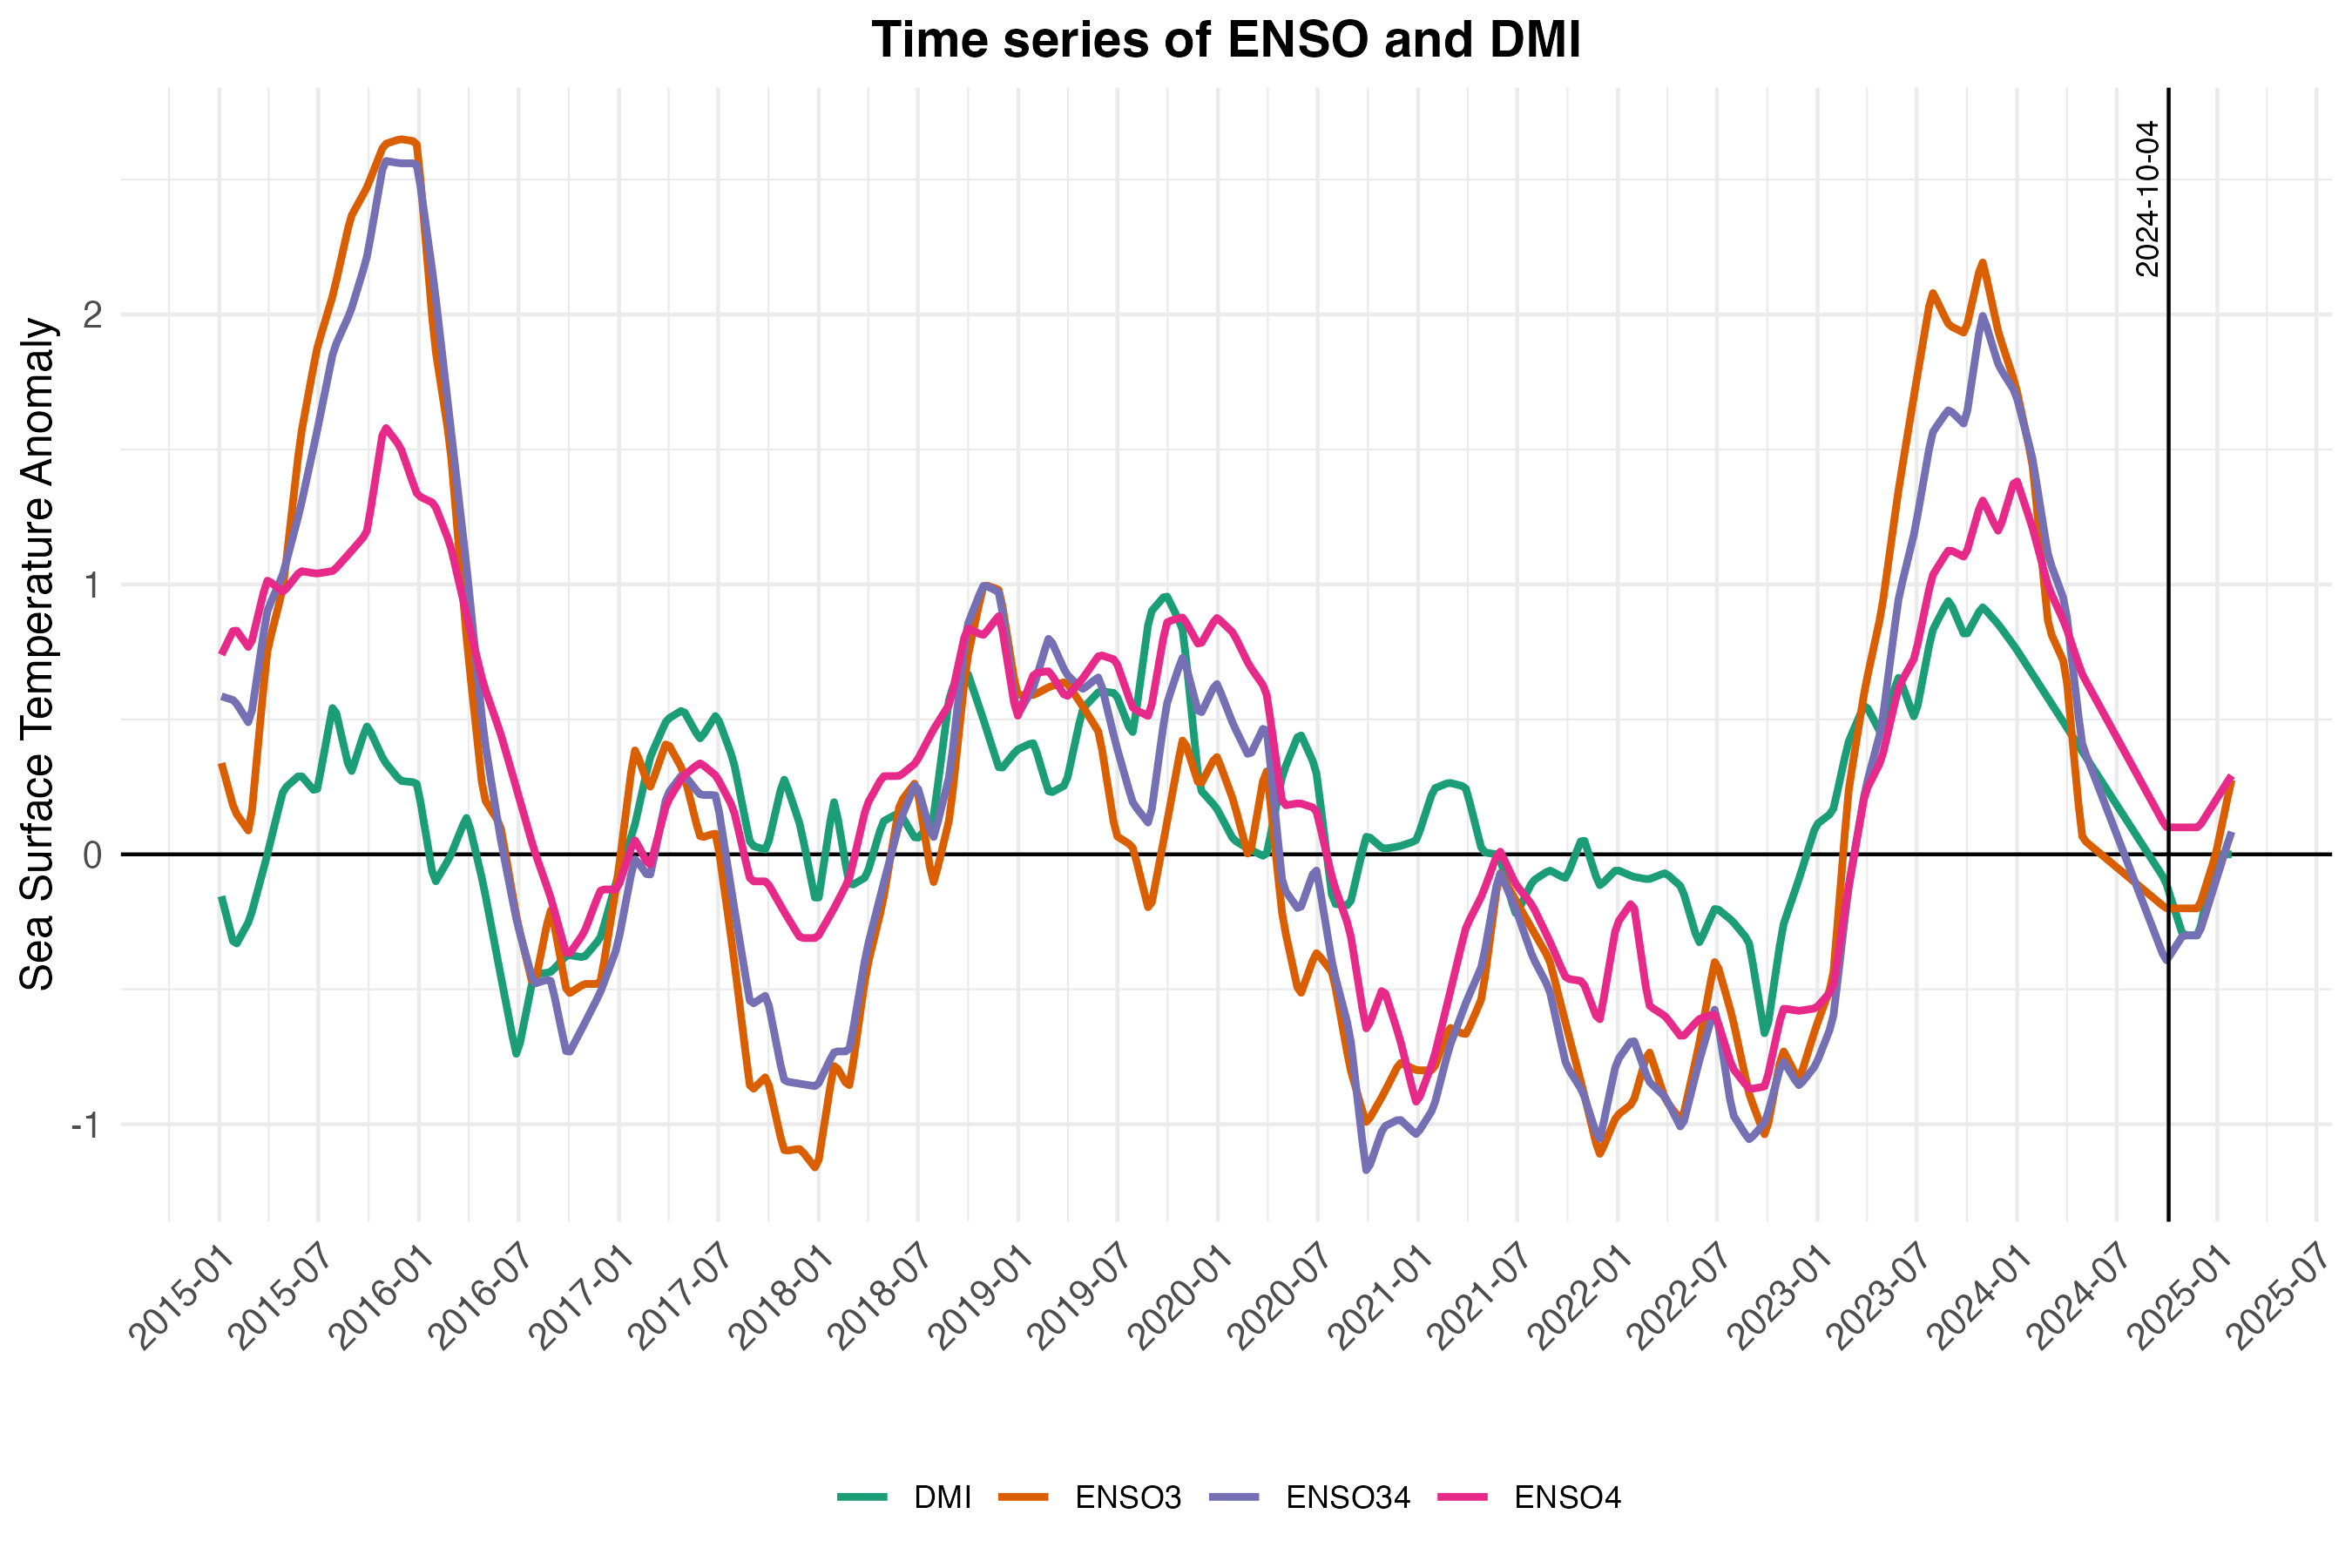
\includegraphics[width=1\linewidth]{figures/climate_data_ENSO_weekly} 

}

\caption{Historical and forecasted values of the Indian Ocean Dipole Mode Index (DMI) and the El Niño Southern Oscillation (ENSO) from 2015 to 2025. The ENSO values come from three different regions: Niño3 (central to eastern Pacific), Niño3.4 (central Pacific), and Niño4 (western-central Pacifi). Data are from National Oceanic and Atmospheric Administration (NOAA) and Bureau of Meteorology (BOM).}\label{fig:climate-data-enso}
\end{figure}

\begin{table}

\caption{\label{tab:climate-data-variables}A full list of covariates and their sources used in the LSTM RNN model to predict the environmental suitability of *V. cholerae* ($\psi_{jt}$).}
\centering
\begin{tabular}[t]{l|l|l}
\hline
Covariate & Description & Source\\
\hline
temperature\_2m\_mean & Average temperature at 2 meters & OpenMeteo [Historical Weather](https://open-meteo.com/en/docs/historical-weather-api) and [Climate Change](https://open-meteo.com/en/docs/climate-api) APIs\\
\hline
temperature\_2m\_max & Maximum temperature at 2 meters & OpenMeteo [Historical Weather](https://open-meteo.com/en/docs/historical-weather-api) and [Climate Change](https://open-meteo.com/en/docs/climate-api) APIs\\
\hline
temperature\_2m\_min & Minimum temperature at 2 meters & OpenMeteo [Historical Weather](https://open-meteo.com/en/docs/historical-weather-api) and [Climate Change](https://open-meteo.com/en/docs/climate-api) APIs\\
\hline
wind\_speed\_10m\_mean & Average wind speed at 10 meters & OpenMeteo [Historical Weather](https://open-meteo.com/en/docs/historical-weather-api) and [Climate Change](https://open-meteo.com/en/docs/climate-api) APIs\\
\hline
wind\_speed\_10m\_max & Maximum wind speed at 10 meters & OpenMeteo [Historical Weather](https://open-meteo.com/en/docs/historical-weather-api) and [Climate Change](https://open-meteo.com/en/docs/climate-api) APIs\\
\hline
cloud\_cover\_mean & Mean cloud cover & OpenMeteo [Historical Weather](https://open-meteo.com/en/docs/historical-weather-api) and [Climate Change](https://open-meteo.com/en/docs/climate-api) APIs\\
\hline
shortwave\_radiation\_sum & Total shortwave radiation & OpenMeteo [Historical Weather](https://open-meteo.com/en/docs/historical-weather-api) and [Climate Change](https://open-meteo.com/en/docs/climate-api) APIs\\
\hline
relative\_humidity\_2m\_mean & Mean relative humidity at 2 meters & OpenMeteo [Historical Weather](https://open-meteo.com/en/docs/historical-weather-api) and [Climate Change](https://open-meteo.com/en/docs/climate-api) APIs\\
\hline
relative\_humidity\_2m\_max & Maximum relative humidity at 2 meters & OpenMeteo [Historical Weather](https://open-meteo.com/en/docs/historical-weather-api) and [Climate Change](https://open-meteo.com/en/docs/climate-api) APIs\\
\hline
relative\_humidity\_2m\_min & Minimum relative humidity at 2 meters & OpenMeteo [Historical Weather](https://open-meteo.com/en/docs/historical-weather-api) and [Climate Change](https://open-meteo.com/en/docs/climate-api) APIs\\
\hline
dew\_point\_2m\_mean & Mean dew point at 2 meters & OpenMeteo [Historical Weather](https://open-meteo.com/en/docs/historical-weather-api) and [Climate Change](https://open-meteo.com/en/docs/climate-api) APIs\\
\hline
dew\_point\_2m\_min & Minimum dew point at 2 meters & OpenMeteo [Historical Weather](https://open-meteo.com/en/docs/historical-weather-api) and [Climate Change](https://open-meteo.com/en/docs/climate-api) APIs\\
\hline
dew\_point\_2m\_max & Maximum dew point at 2 meters & OpenMeteo [Historical Weather](https://open-meteo.com/en/docs/historical-weather-api) and [Climate Change](https://open-meteo.com/en/docs/climate-api) APIs\\
\hline
precipitation\_sum & Total precipitation & OpenMeteo [Historical Weather](https://open-meteo.com/en/docs/historical-weather-api) and [Climate Change](https://open-meteo.com/en/docs/climate-api) APIs\\
\hline
pressure\_msl\_mean & Mean sea level pressure & OpenMeteo [Historical Weather](https://open-meteo.com/en/docs/historical-weather-api) and [Climate Change](https://open-meteo.com/en/docs/climate-api) APIs\\
\hline
soil\_moisture\_0\_to\_10cm\_mean & Mean soil moisture at 0 to 10 cm & OpenMeteo [Historical Weather](https://open-meteo.com/en/docs/historical-weather-api) and [Climate Change](https://open-meteo.com/en/docs/climate-api) APIs\\
\hline
et0\_fao\_evapotranspiration\_sum & Total evapotranspiration (FAO method) & OpenMeteo [Historical Weather](https://open-meteo.com/en/docs/historical-weather-api) and [Climate Change](https://open-meteo.com/en/docs/climate-api) APIs\\
\hline
DMI & Dipole Mode Index (DMI) & [NOAA](https://psl.noaa.gov/enso/) and [BOM](http://www.bom.gov.au/climate/ocean/outlooks/\#region=NINO4\&region=NINO3\&region=NINO34)\\
\hline
ENSO3 & El Niño Southern Oscillation (ENSO) - Region 3 & [NOAA](https://psl.noaa.gov/enso/) and [BOM](http://www.bom.gov.au/climate/ocean/outlooks/\#region=NINO4\&region=NINO3\&region=NINO34)\\
\hline
ENSO34 & ENSO - Region 3.4 & [NOAA](https://psl.noaa.gov/enso/) and [BOM](http://www.bom.gov.au/climate/ocean/outlooks/\#region=NINO4\&region=NINO3\&region=NINO34)\\
\hline
ENSO4 & ENSO - Region 4 & [NOAA](https://psl.noaa.gov/enso/) and [BOM](http://www.bom.gov.au/climate/ocean/outlooks/\#region=NINO4\&region=NINO3\&region=NINO34)\\
\hline
elevation & Mean elevation & [Amazon Web Services Terrain Tiles](https://registry.opendata.aws/terrain-tiles/)\\
\hline
\end{tabular}
\end{table}

\subsubsection{Deep learning neural network model}\label{deep-learning-neural-network-model}

As mentioned above, we model environmental suitability \(\psi_{jt}\) using a Long Short-Term Memory (LSTM) Recurrent Neural Network (RNN) model. The LSTM model was developed using \href{https://cran.r-project.org/package=keras}{\texttt{keras}} and \href{https://cran.r-project.org/package=tensorflow}{\texttt{tensorflow}} in R to predict binary outcomes. Thus the modeled quantity \(\psi_{jt}\) is a proportion implying unsuitable conditions at 0 and perfectly suitable conditions at 1.

The model was fitted to reported case counts that were converted to a binary variable using a threshold of 200 reported cases per week. Given delays in reporting and likely lead times for environmental suitability ahead of transmission and case reporting, we also set the preceding one week to be suitable and in cases where there were two consecutive weeks of \textgreater200 cases per week, we assumed that the preceding two weeks were also suitable. See Figure \ref{fig:cases-binary} for an example of how reported case counts are converted to a binary variable representing presumed environmental suitability for \emph{V. cholerae}.

\begin{figure}

{\centering 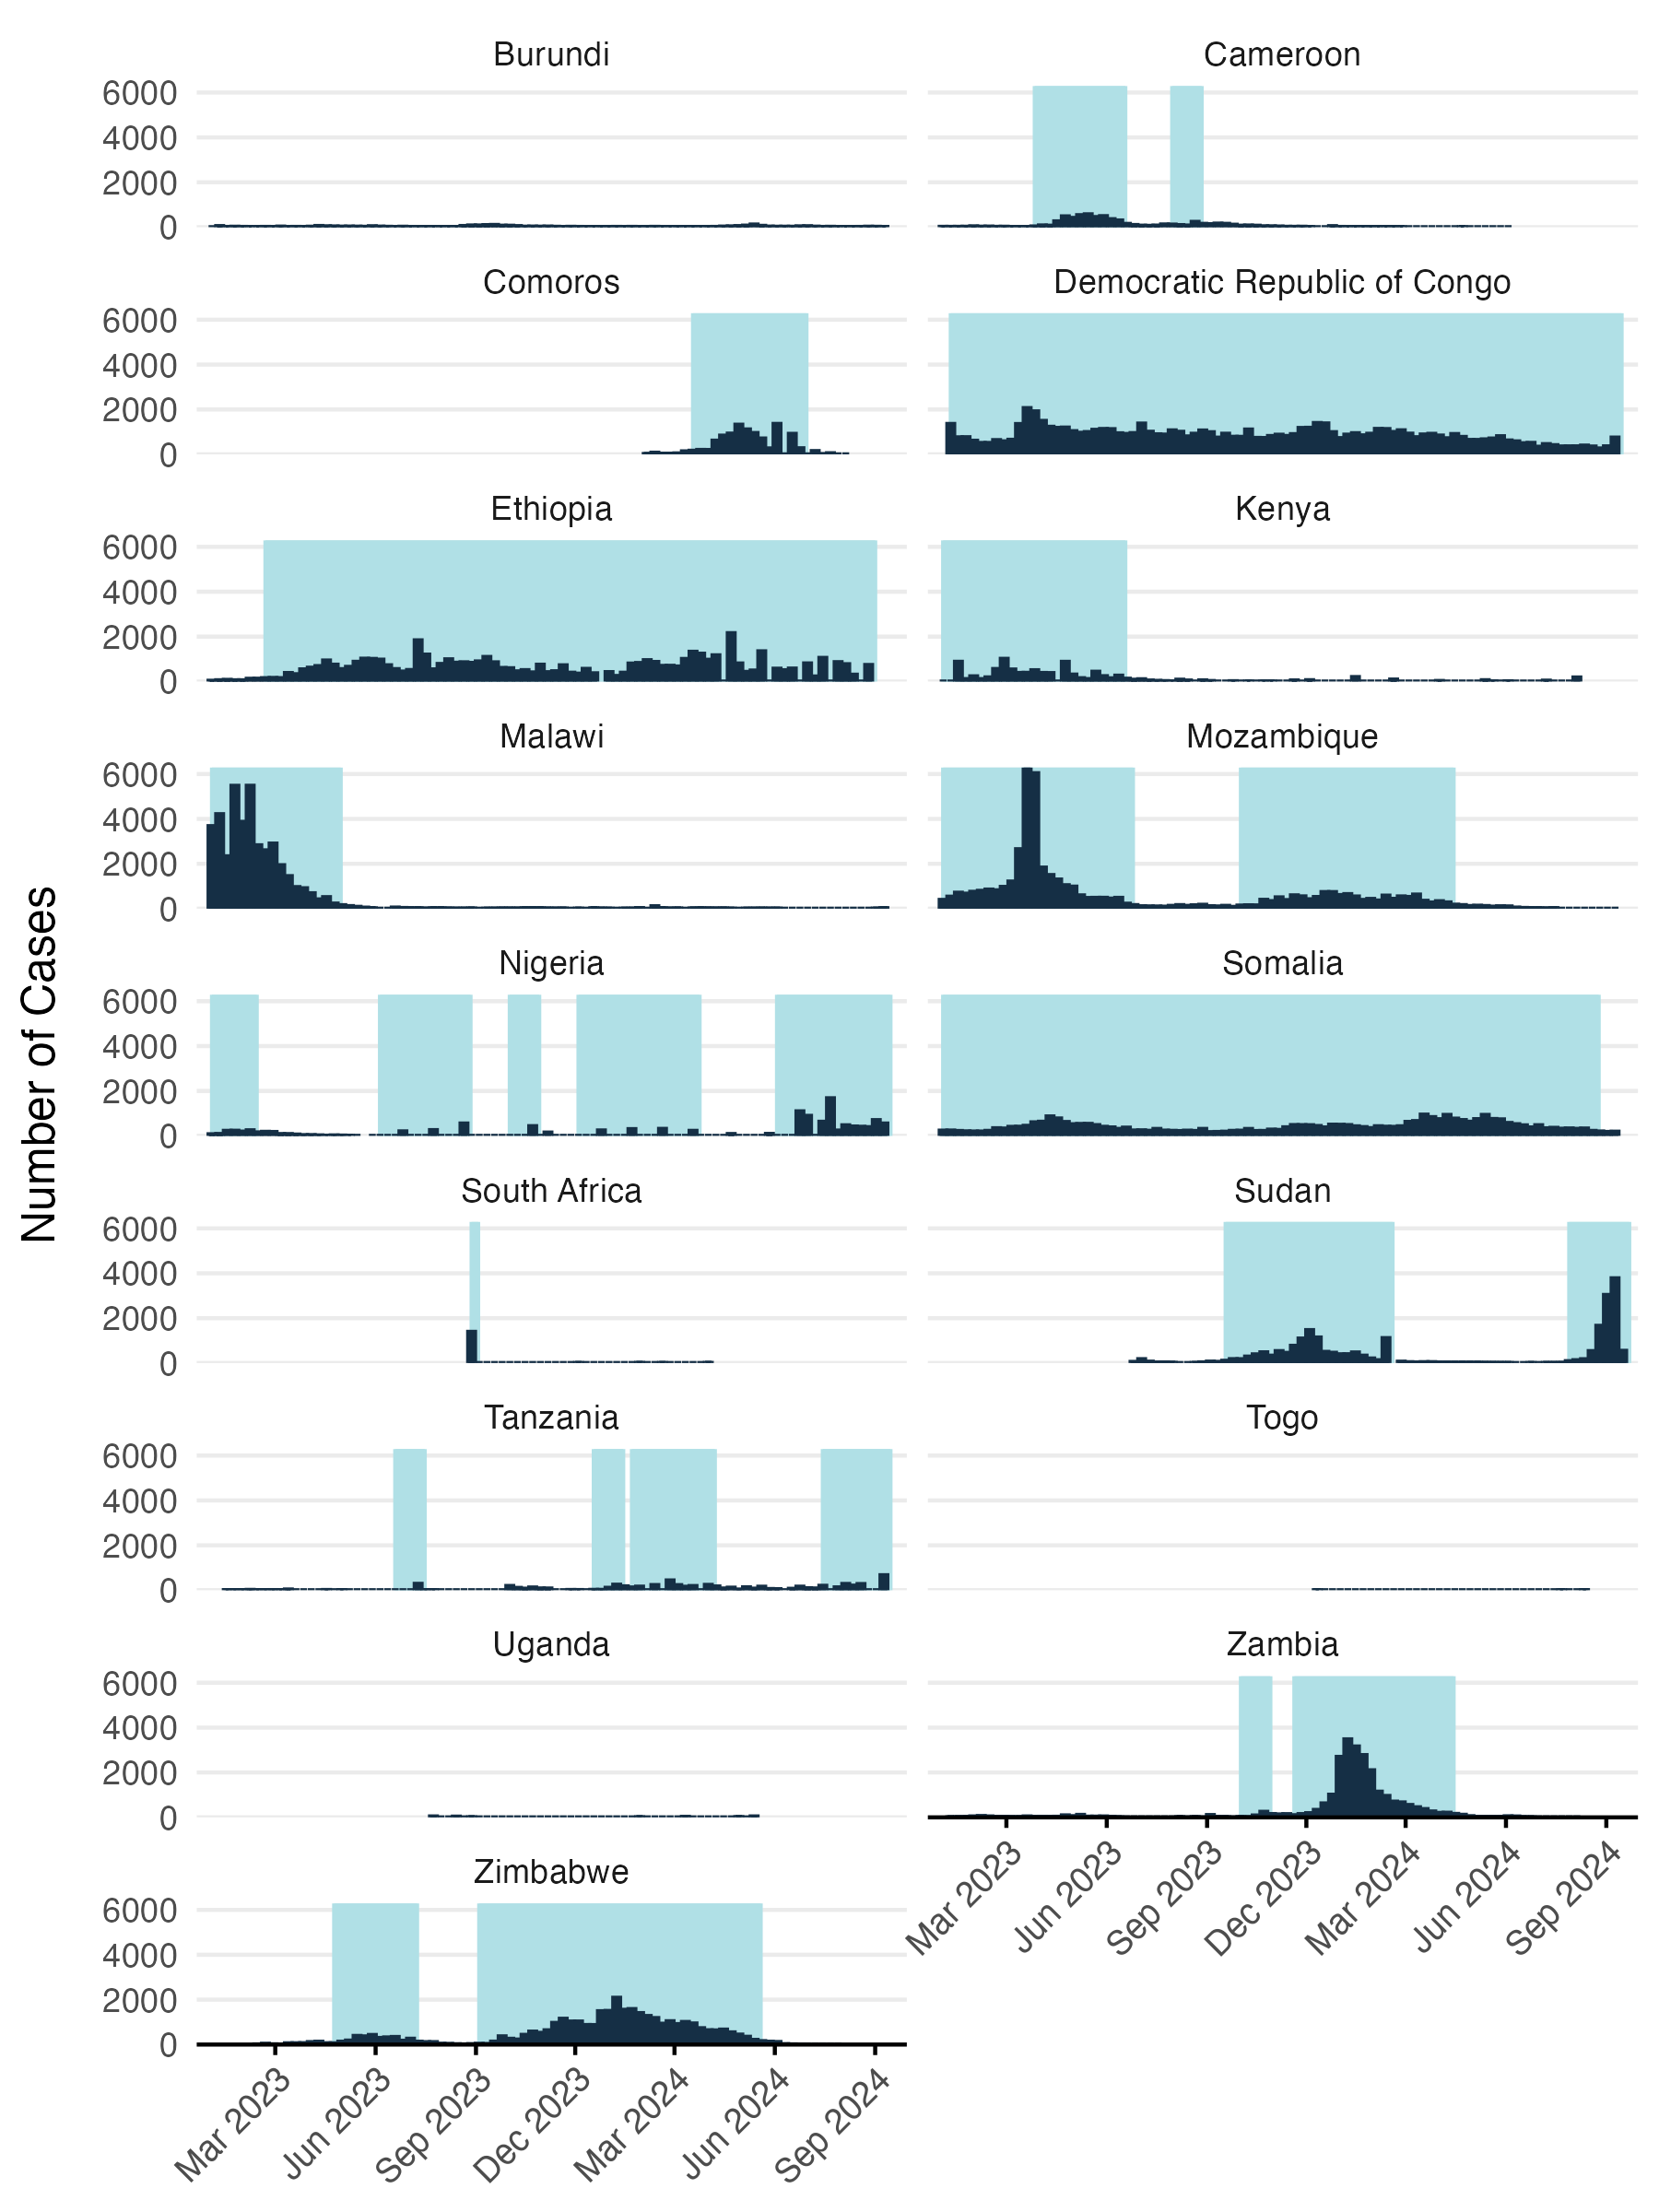
\includegraphics[width=1\linewidth]{figures/cases_binary} 

}

\caption{Reported cases converted to binary variable for modeling environmental suitability.}\label{fig:cases-binary}
\end{figure}

The model is a Long Short-Term Memory (LSTM) neural network designed for binary classification, where environmental suitability, \(\psi_{jt}\), is modeled as a function of the hidden state \(h_t\) and hidden bias term \(b_h\). Specifically, \(\psi_{jt}\) is defined by a sigmoid activation function applied to the linear combination of the hidden state \(h_t\) and the bias \(b_h\) which if given by the 3 layers of the LSTM model:

\begin{equation}
\psi_{jt} \sim \text{Sigmoid}(w_h \cdot h_t + b_h)
\label{eq:psi}
\end{equation}

\begin{equation}
h_t = \text{LSTM}\big(\text{temperature}_{jt}, \ \text{precipitation}_{jt}, \ \text{ENSO}_{t}, \dots \big)
\end{equation}

In this formulation, \(h_t\) represents the hidden state generated by the LSTM network based on input variables such as temperature, precipitation, and ENSO conditions, while \(b_h\) is a bias term added to the output of the hidden state transformation.

The deep learning LSTM model consists of three stacked LSTM-RNN layers. The first LSTM layer has 500 units and the second and third LSTM layers have 250 and 100 units respectively. The architecture the LSTM model is configured to pass node values to subsequent LSTM layers allowing deep learning of more the complex interactions among the climate variable over time. We enforced model sparsity for each LSTM layer using L2 regularization (penalty = 0.001) and used a dropout rate of 0.5 for each LSTM layer to further prevent overfitting on the limited amount of data. The final output layer was a dense layer with a single unit and a sigmoid activation function to produce a probability value for binary classification, i.e.~a prediction of environmental suitability \(\psi_{jt}\) on a scale of 0 to 1.

To fit the LSTM model to data, we modified the learning rate by applying an exponential decay schedule that started at 0.001 and decayed by a factor of 0.9 every 10,000 steps to enable smoother convergence. The model was compiled using the Adam optimizer with this learning rate schedule, along with binary cross-entropy as the loss function and accuracy as the evaluation metric. The model was trained for a maximum of 200 epochs with a batch size of 1024. We allowed model fitting to stop early with a patience parameter of 10 which halts training if no improvement is observed in validation accuracy for 10 consecutive epochs. To train the model we set aside 20\% of the observed data for validation and also used 20\% of the training data for model fitting. The training history, including loss and accuracy, was monitored over the course of training and gave a final test accuracy of 0.73 and a final test loss of 0.56 (see Figure \ref{fig:lstm-model-fit}).

\begin{figure}

{\centering 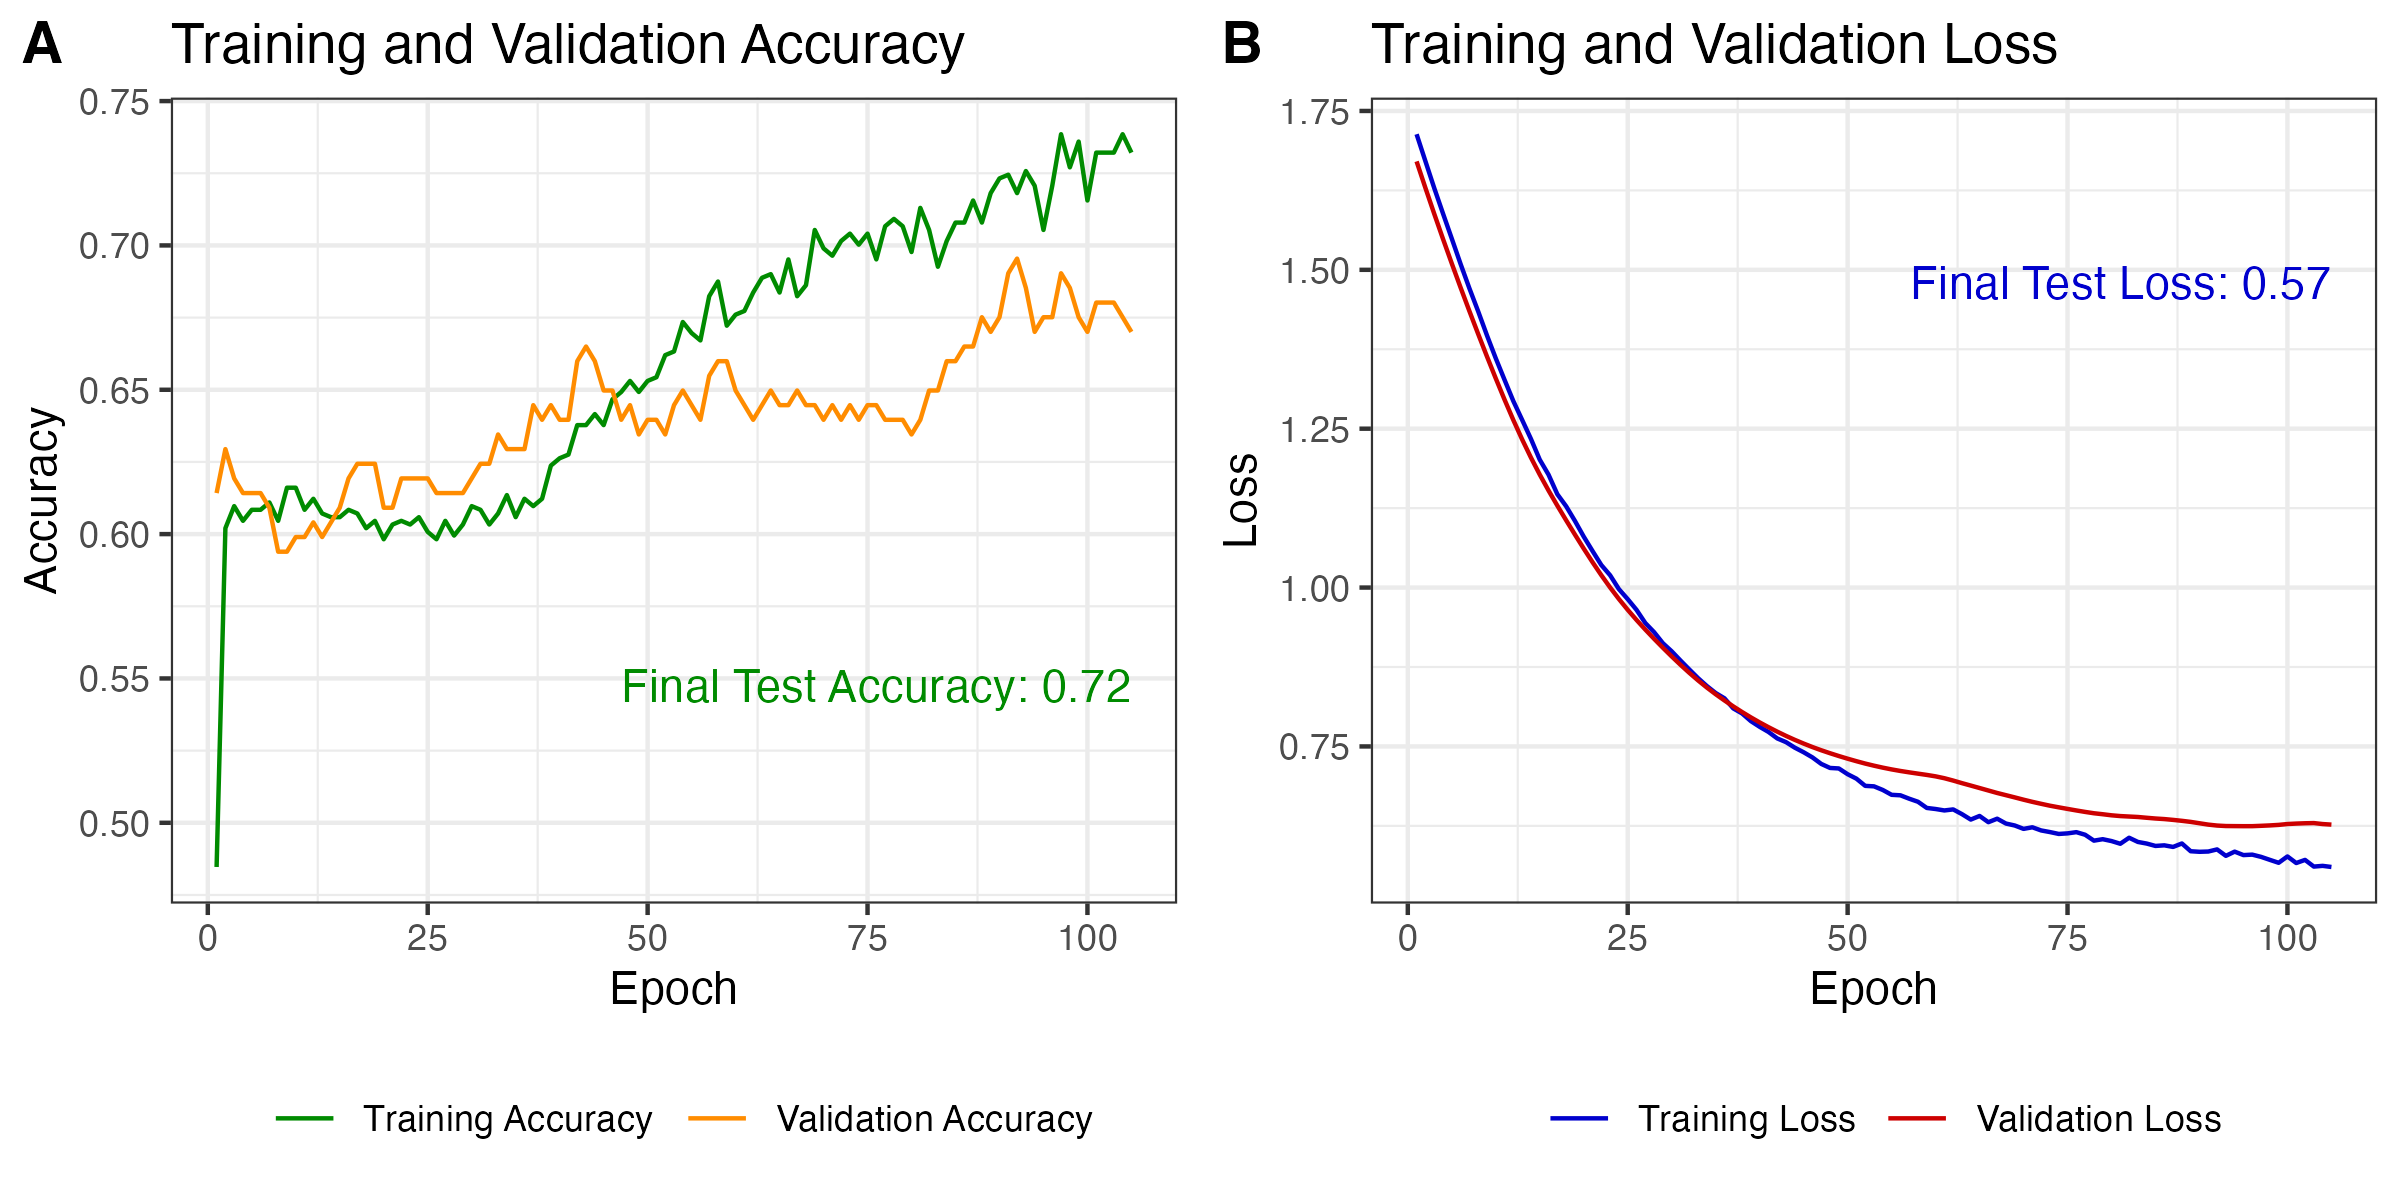
\includegraphics[width=1\linewidth]{figures/suitability_LSTM_fit} 

}

\caption{Model performance on training and validation data.}\label{fig:lstm-model-fit}
\end{figure}

After model training was completed, we predicted the values of environmental suitability \(\psi_{jt}\) across all time steps for each location. Predictions start in January 1970 and go up to 5 months past the present date (currently February 2025). Given the amount of noise in the model predictions, we added a simple LOESS spline with logit transformation to smooth model predictions over time and give a more stable value of \(\psi_{jt}\) when incorporating it into other model features (e.g.~Equations \eqref{eq:beta2} and \eqref{eq:delta}). The resulting model predictions are shown for an example country such as Mozambique in Figure \ref{fig:psi-prediction-data} which compares model predictions to the original case counts and the binary classification. Predicitons for all model locations are shown in a simplified view in Figure \ref{fig:psi-prediction-countries}.

\emph{Also, please note that this initial version of the model is fitted to a rather small amount of data. Model hyper parameters were specifically chosen to reduce overfitting. Therefore, we recommend to not over-interpret the time series predictions of the model at this early stage since they are likely to change and improve as more historical incidence data is included in future versions.}

\begin{figure}

{\centering 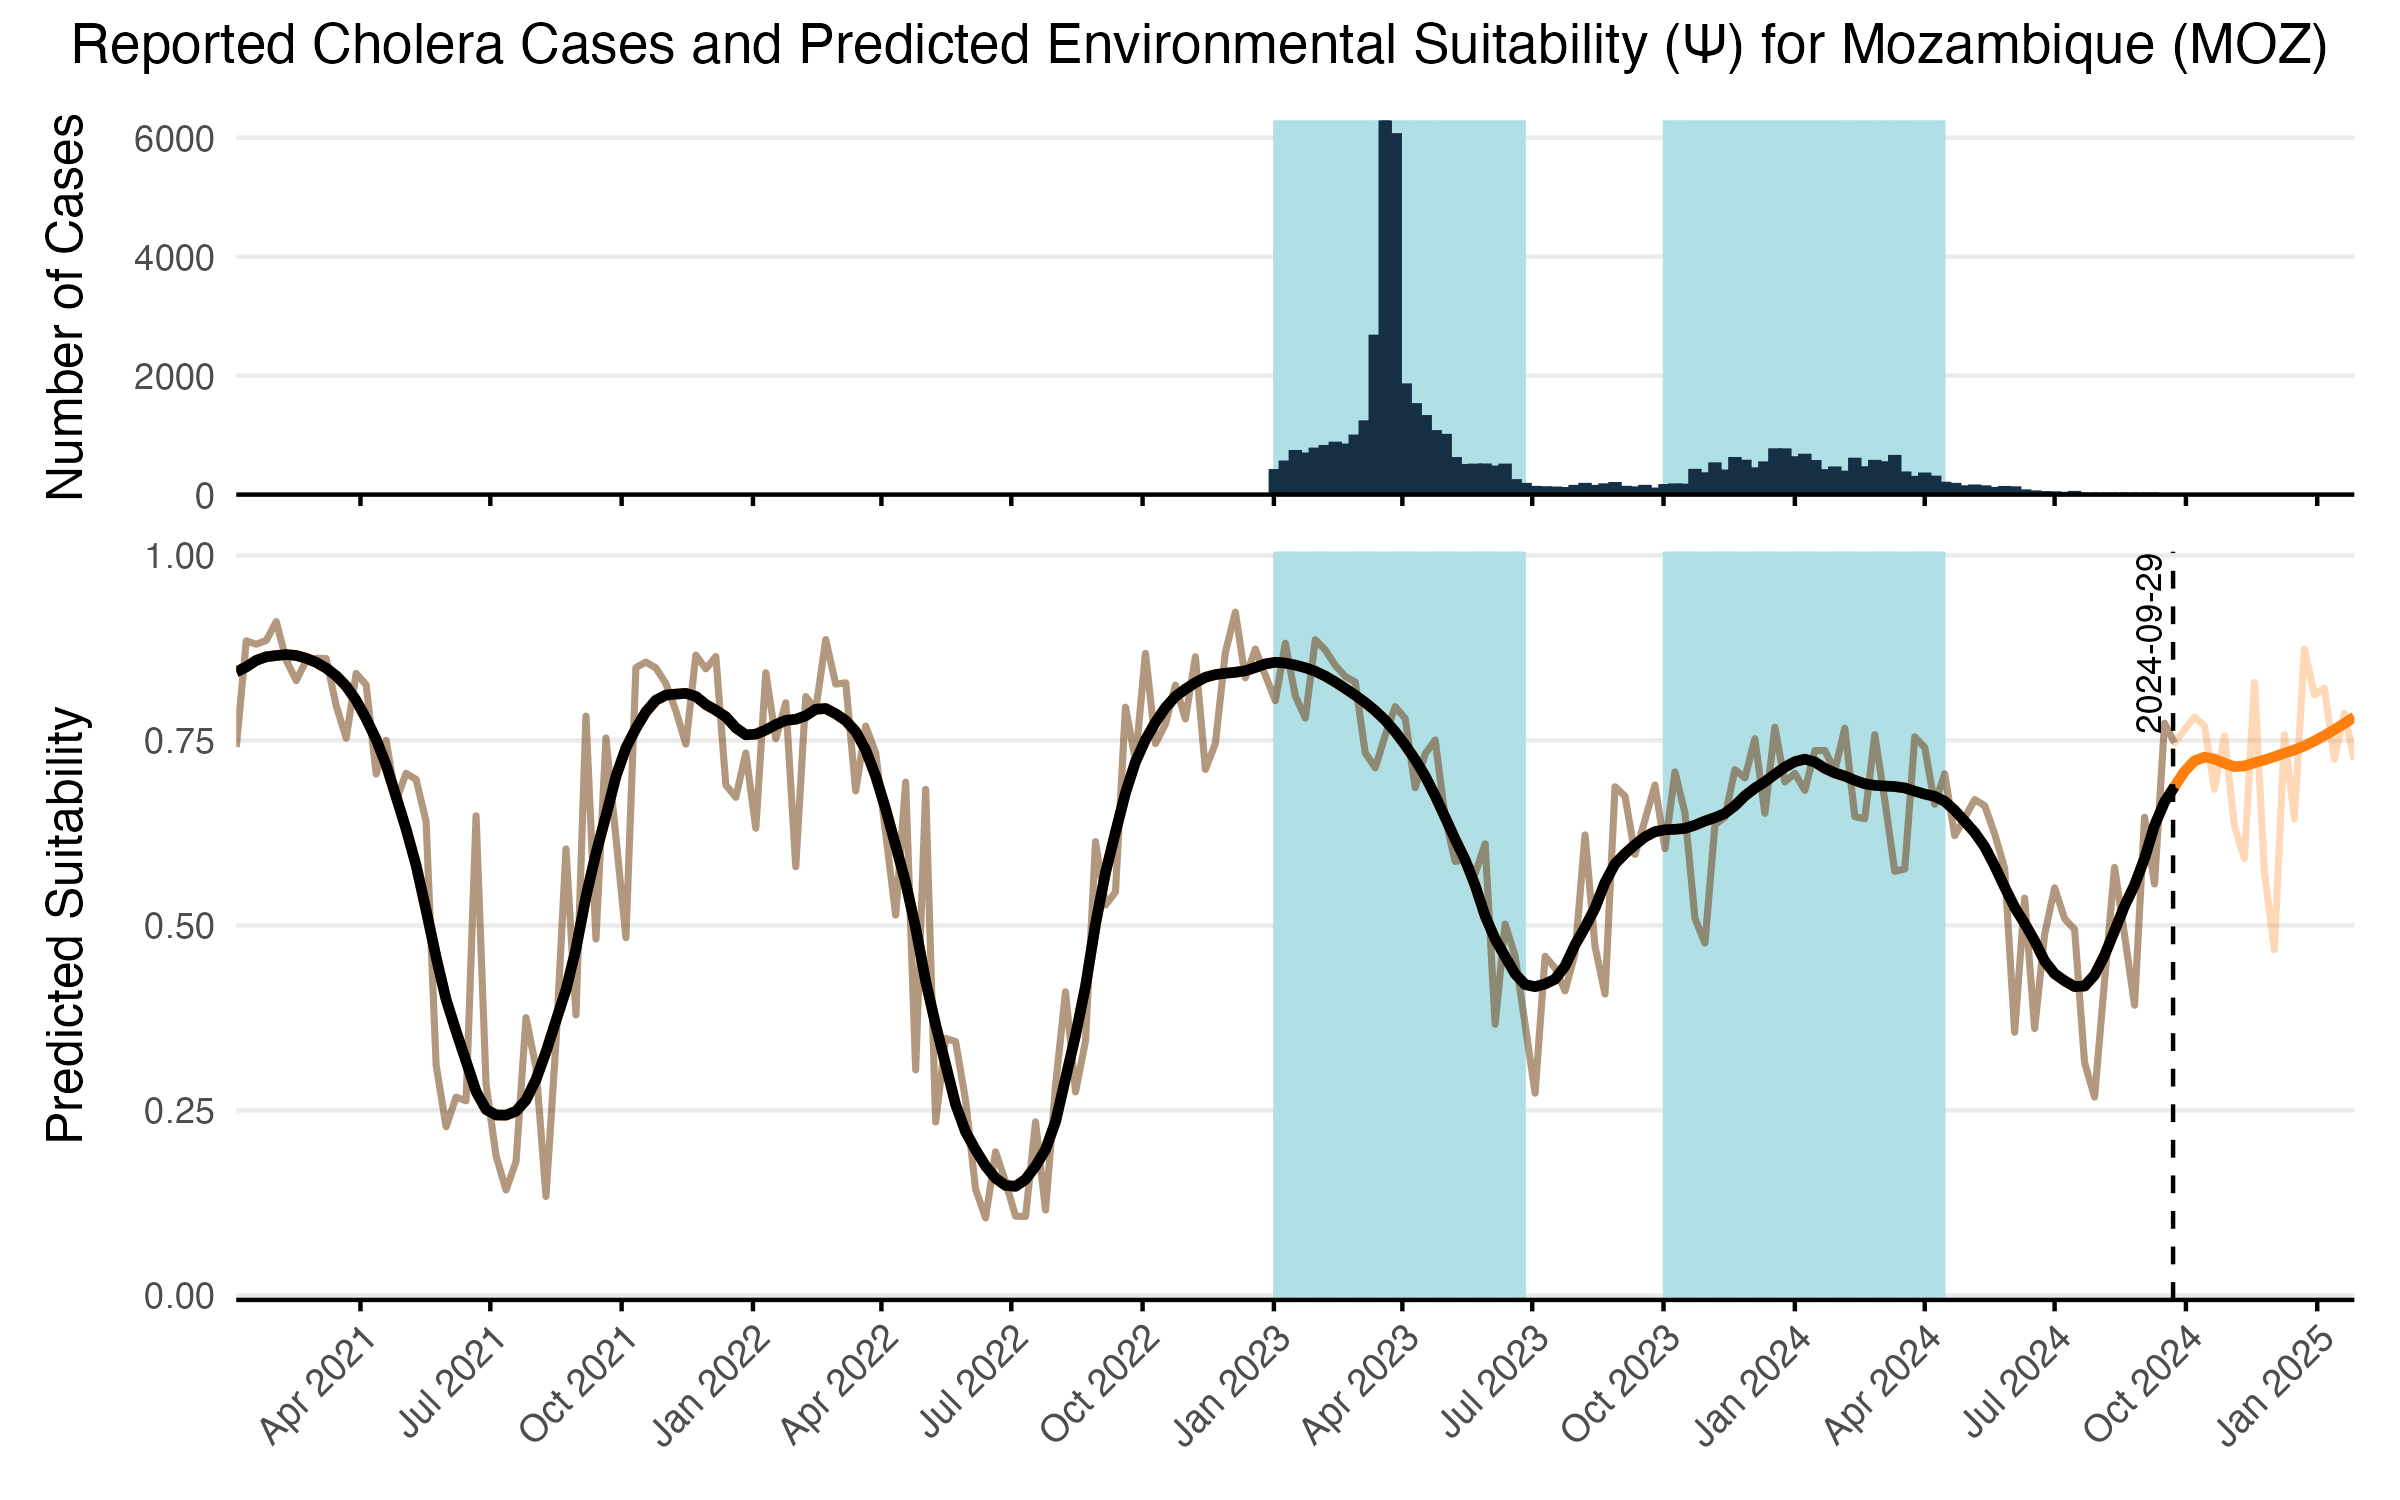
\includegraphics[width=1\linewidth]{figures/suitability_cases_MOZ} 

}

\caption{The LSTM model predictions over time and reported cases for an example country such as Mozambique. Reported cases are shown in the top panel and tje shaded areas show the binary classification used to characterize environmental suitability. Raw model predicitons are shown in the transparent brown line with the solid black line showing the LOESS smoothing. Forecasted values beyond the current time point are shown in orange and are limited to 5 month time horizon.}\label{fig:psi-prediction-data}
\end{figure}

\begin{figure}

{\centering 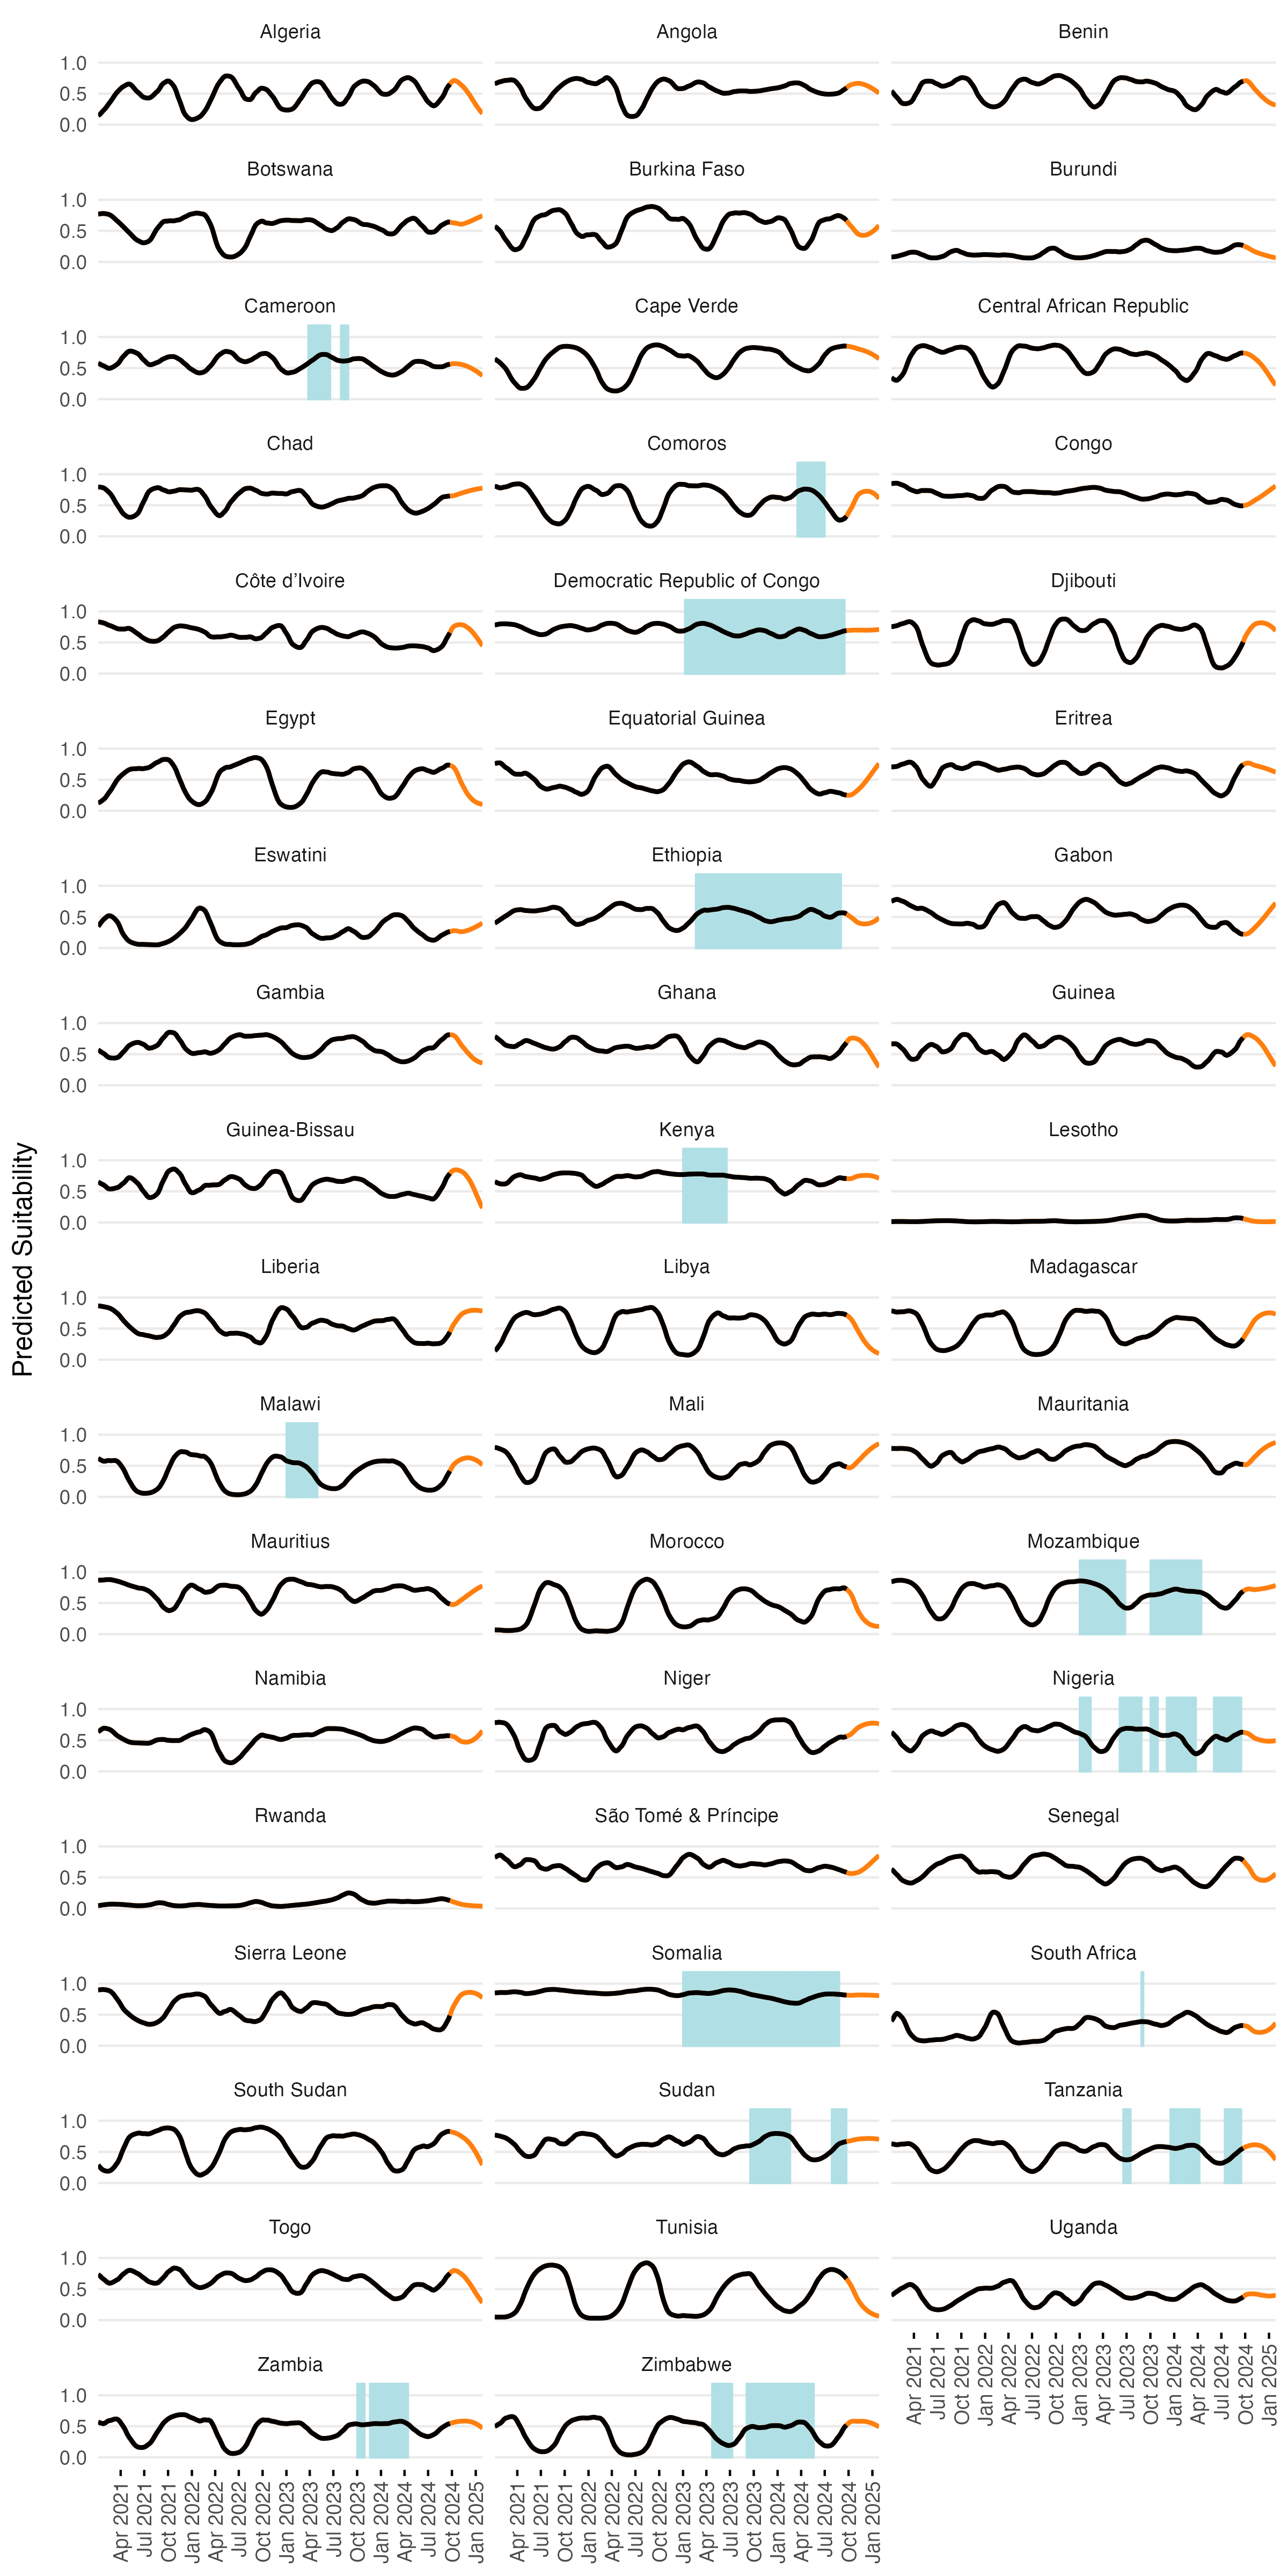
\includegraphics[width=1\linewidth]{figures/suitability_by_country} 

}

\caption{The smoothed LSTM model predictions (lines) and binary suitability classification (shaded areas) over time for all countries in the MOSAIC framework. Orange lines show forecasts beyond the current date. With ENSO and DMI covariates included in the model, forecasts are limited to 5 months.}\label{fig:psi-prediction-countries}
\end{figure}

\subsection{Shedding}\label{shedding}

The rate at which infected individuals shed \emph{V. cholerae} into the environment (\(\zeta\)) is a critical factor influencing cholera transmission. Shedding rates can vary widely depending on the severity of the infection, the immune response of the individual, and environmental factors. According to \href{https://www.ncbi.nlm.nih.gov/pmc/articles/PMC3926264/}{Fung 2014}, the shedding rate is estimated to range from 0.01 to 10 cells per mL per person per day.

Further studies support these findings, indicating that shedding rates can indeed fluctuate significantly. For instance, \href{https://www.ncbi.nlm.nih.gov/pmc/articles/PMC3842031/}{Nelson et al (2009)} note that during the, depending on the phase of infection, individuals can shed \(10^3\) (asymptomatic cases) to \(10^{12}\) (severe cases) \emph{V. cholerae} cells per gram of stool. Future version of the model may attempt to capture the nuances of shedding dynamics, but here we make the simplifying assumption that shedding is constant across infected individuals and has a wide range of variability with no prior distributional assumptions:

\[
\zeta \sim \text{Uniform}(0.01, 10).
\]

\subsection{WAter, Sanitation, and Hygiene (WASH)}\label{water-sanitation-and-hygiene-wash}

Since \emph{V. cholerae} is transmitted through fecal contamination of water and other consumables, the level of exposure to contaminated substrates significantly impacts transmission rates. Interventions involving Water, Sanitation, and Hygiene (WASH) have long been a first line of defense in reducing cholera transmission, and in this context, WASH variables can serve as proxy for the rate of contact with environmental risk factors. In the MOSAIC model, WASH variables are incorporated mechanistically, allowing for intervention scenarios that include changes to WASH. However, it is necessary to distill available WASH variables into a single parameter that represents the WASH-determined contact rate with contaminated substrates for each location \(j\), which we define as \(\theta_j\).

To parameterize \(\theta_j\), we calculated a weighted mean of the 8 WASH variables in \href{https://doi.org/10.1021/acs.est.3c01317}{Sikder et al 2023} and originally modeled by the \href{https://www.thelancet.com/journals/langlo/article/PIIS2214-109X(20)30278-3/fulltext}{Local Burden of Disease WaSH Collaborators 2020}. The 8 WASH variables (listed in Table \ref{tab:wash-weights}) provide population-weighted measures of the proportion of the population that either: \emph{i}) have access to WASH resources (e.g., piped water, septic or sewer sanitation), or \emph{ii}) are exposed to risk factors (e.g.~surface water, open defecation). For risk associated WASH variables, we used the complement (\(1-\text{value}\)) to give the proportion of the population \emph{not} exposed to each risk factor. We used the \href{https://www.rdocumentation.org/packages/stats/versions/3.6.2/topics/optim}{\texttt{optim}} function in R and the \href{https://en.wikipedia.org/wiki/Limited-memory_BFGS}{L-BFGS-B} algorithm to estimate the set of optimal weights (Table \ref{tab:wash-weights}) that maximize the correlation between the weighted mean of the 8 WASH variables and reported cholera incidence per 1000 population across 40 SSA countries from 2000 to 2016. The optimal weighted mean had a correlation coefficient of \(r =\) -0.33 (-0.51 to -0.09 95\% CI) which was higher than the basic mean and all correlations provided by the individual WASH variables (see Figure \ref{fig:wash-incidence}). The weighted mean then provides a single variable between 0 and 1 that represents the overall proportion of the population that has access to WASH and/or is not exposed to environmental risk factors. Thus, the WASH-mediated contact rate with sources of environmental transmission is represented as (\(1-\theta_j\)) in the environment-to-human force of infection (\(\Psi_{jt}\)). Values of \(\theta_j\) for all countries are shown in Figure \ref{fig:wash-country}.

\begin{table}
\centering
\caption{\label{tab:wash-weights}Table of optimized weights used to calculate the single mean WASH index for all countries.}
\centering
\begin{tabular}[t]{l|r}
\hline
WASH variable & Optimized weight\\
\hline
Piped Water & 0.356\\
\hline
Septic or Sewer Sanitation & 0.014\\
\hline
Other Improved Water & 0.000\\
\hline
Other Improved Sanitation & 0.000\\
\hline
Surface Water & 0.504\\
\hline
Unimproved Sanitation & 0.000\\
\hline
Unimproved Water & 0.000\\
\hline
Open Defecation & 0.126\\
\hline
\end{tabular}
\end{table}

\begin{figure}

{\centering 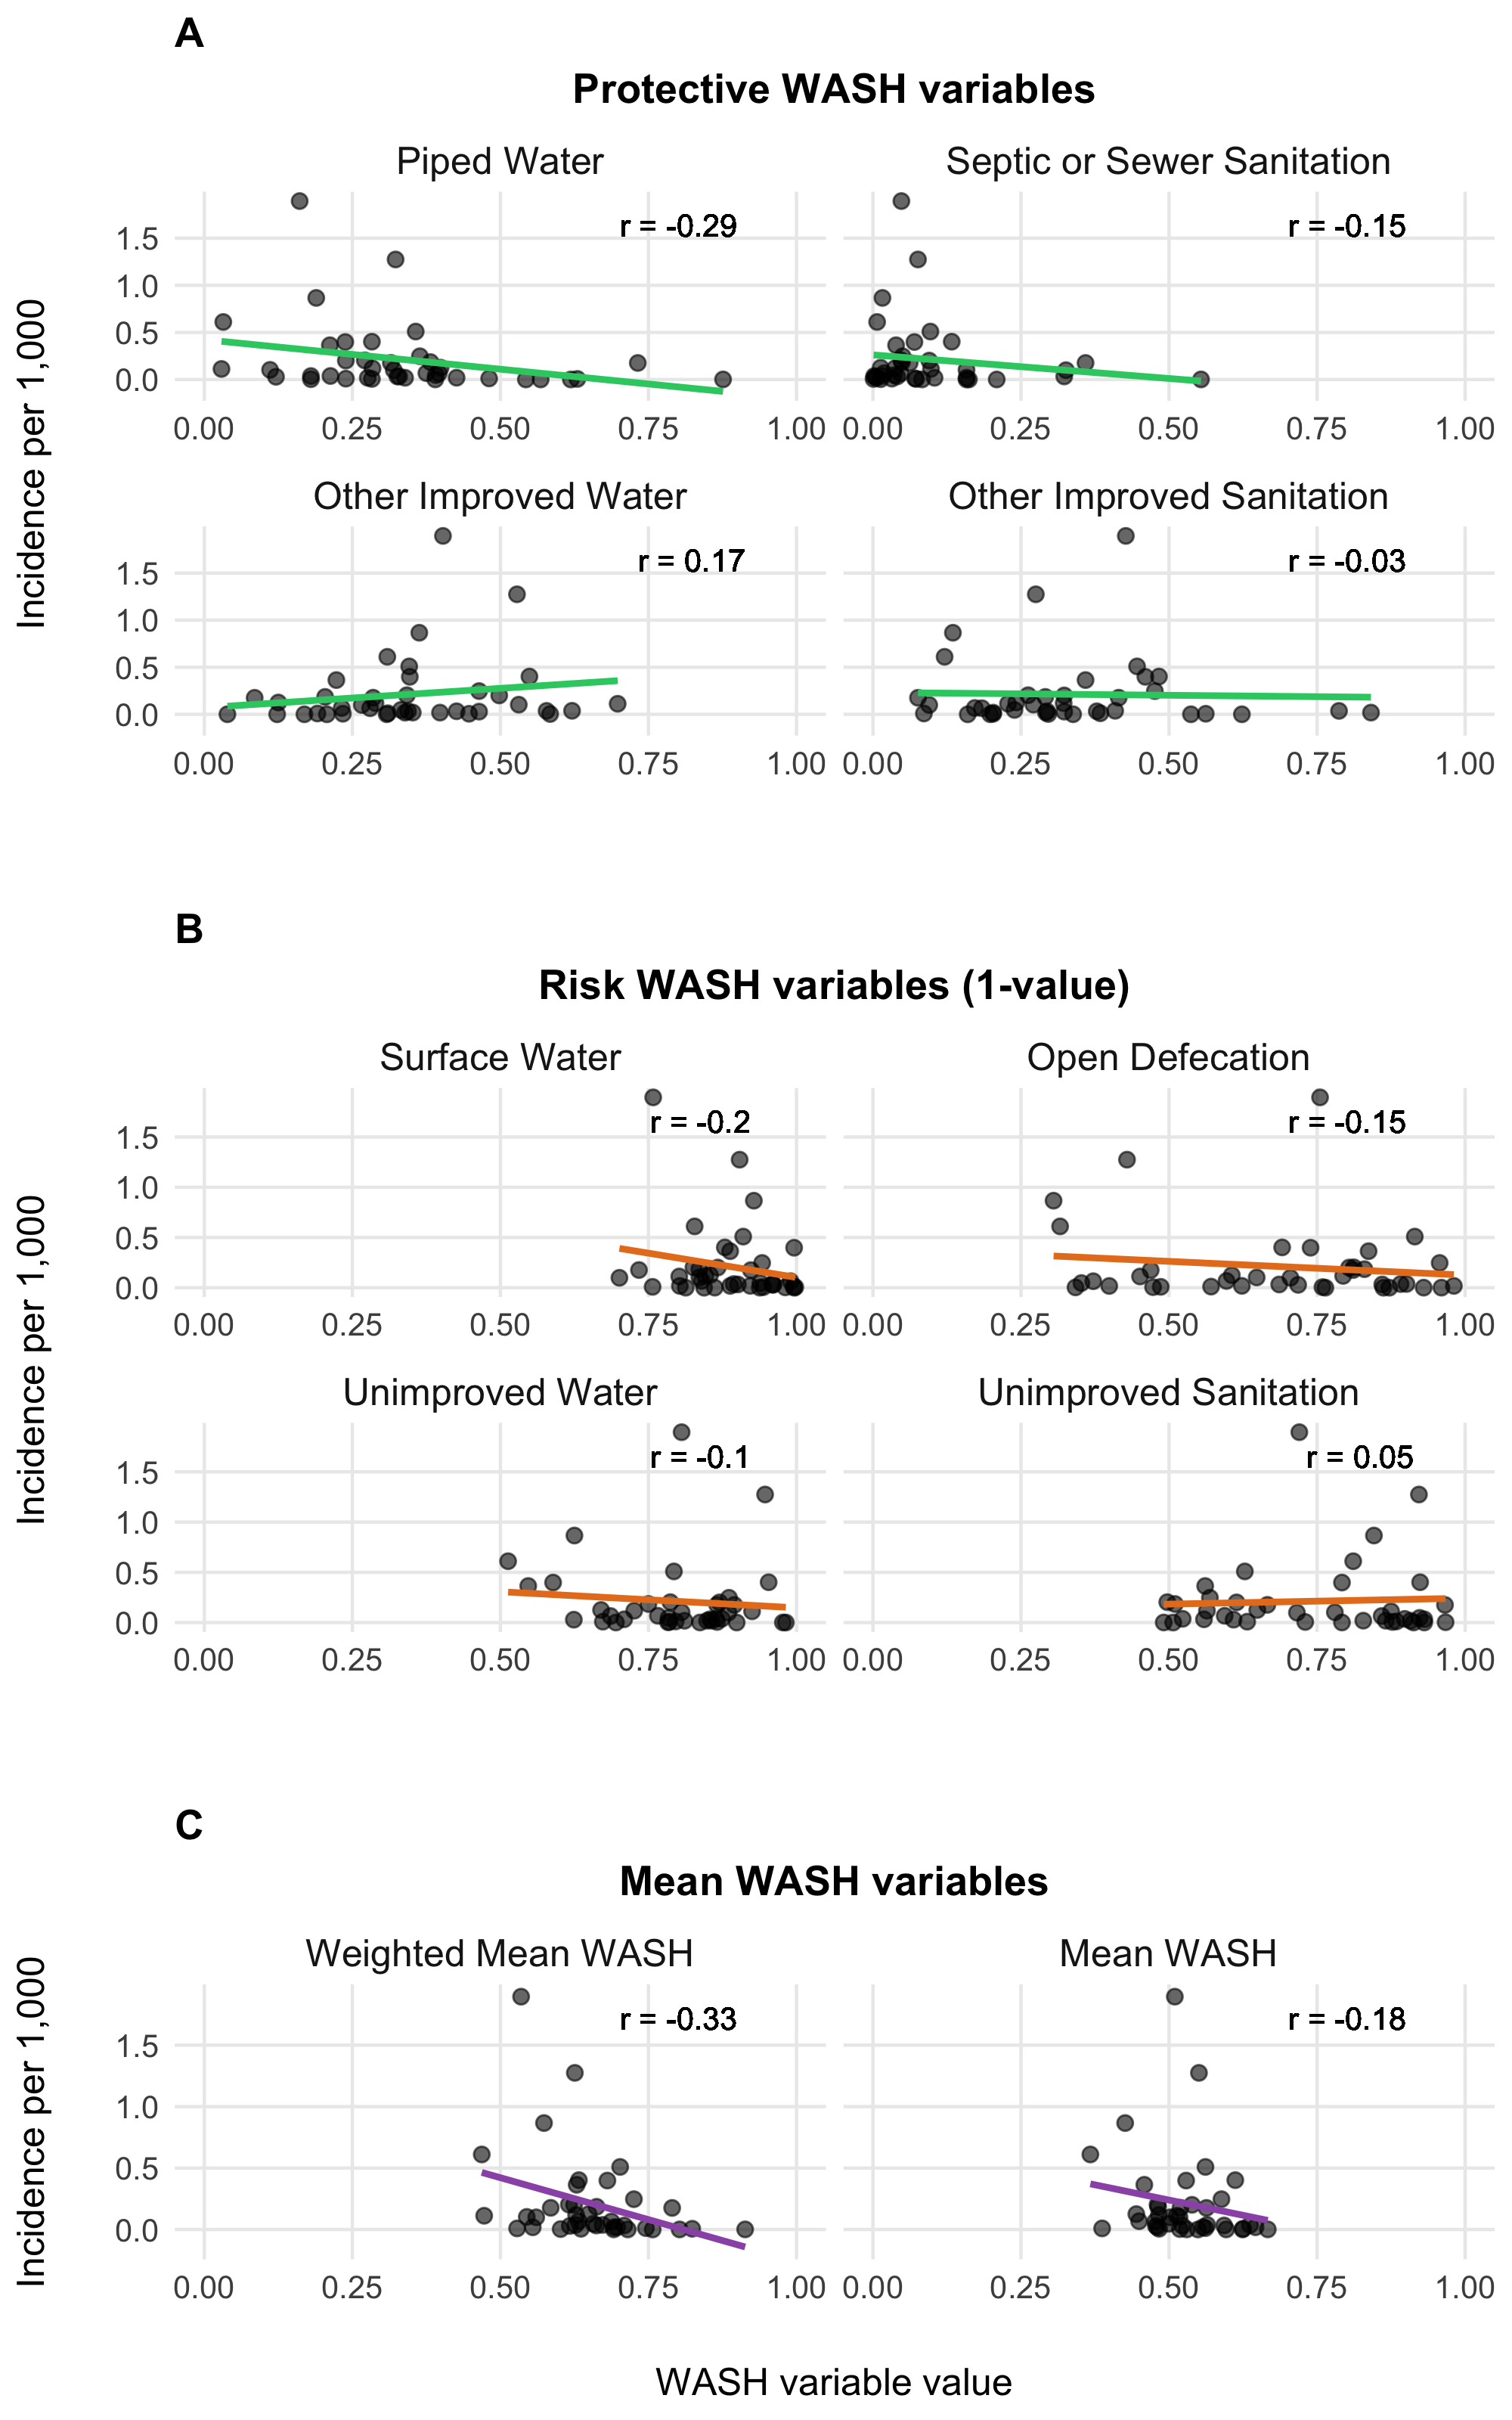
\includegraphics[width=1\linewidth]{figures/wash_incidence_correlation} 

}

\caption{Relationship between WASH variables and cholera incidences.}\label{fig:wash-incidence}
\end{figure}

\begin{figure}

{\centering 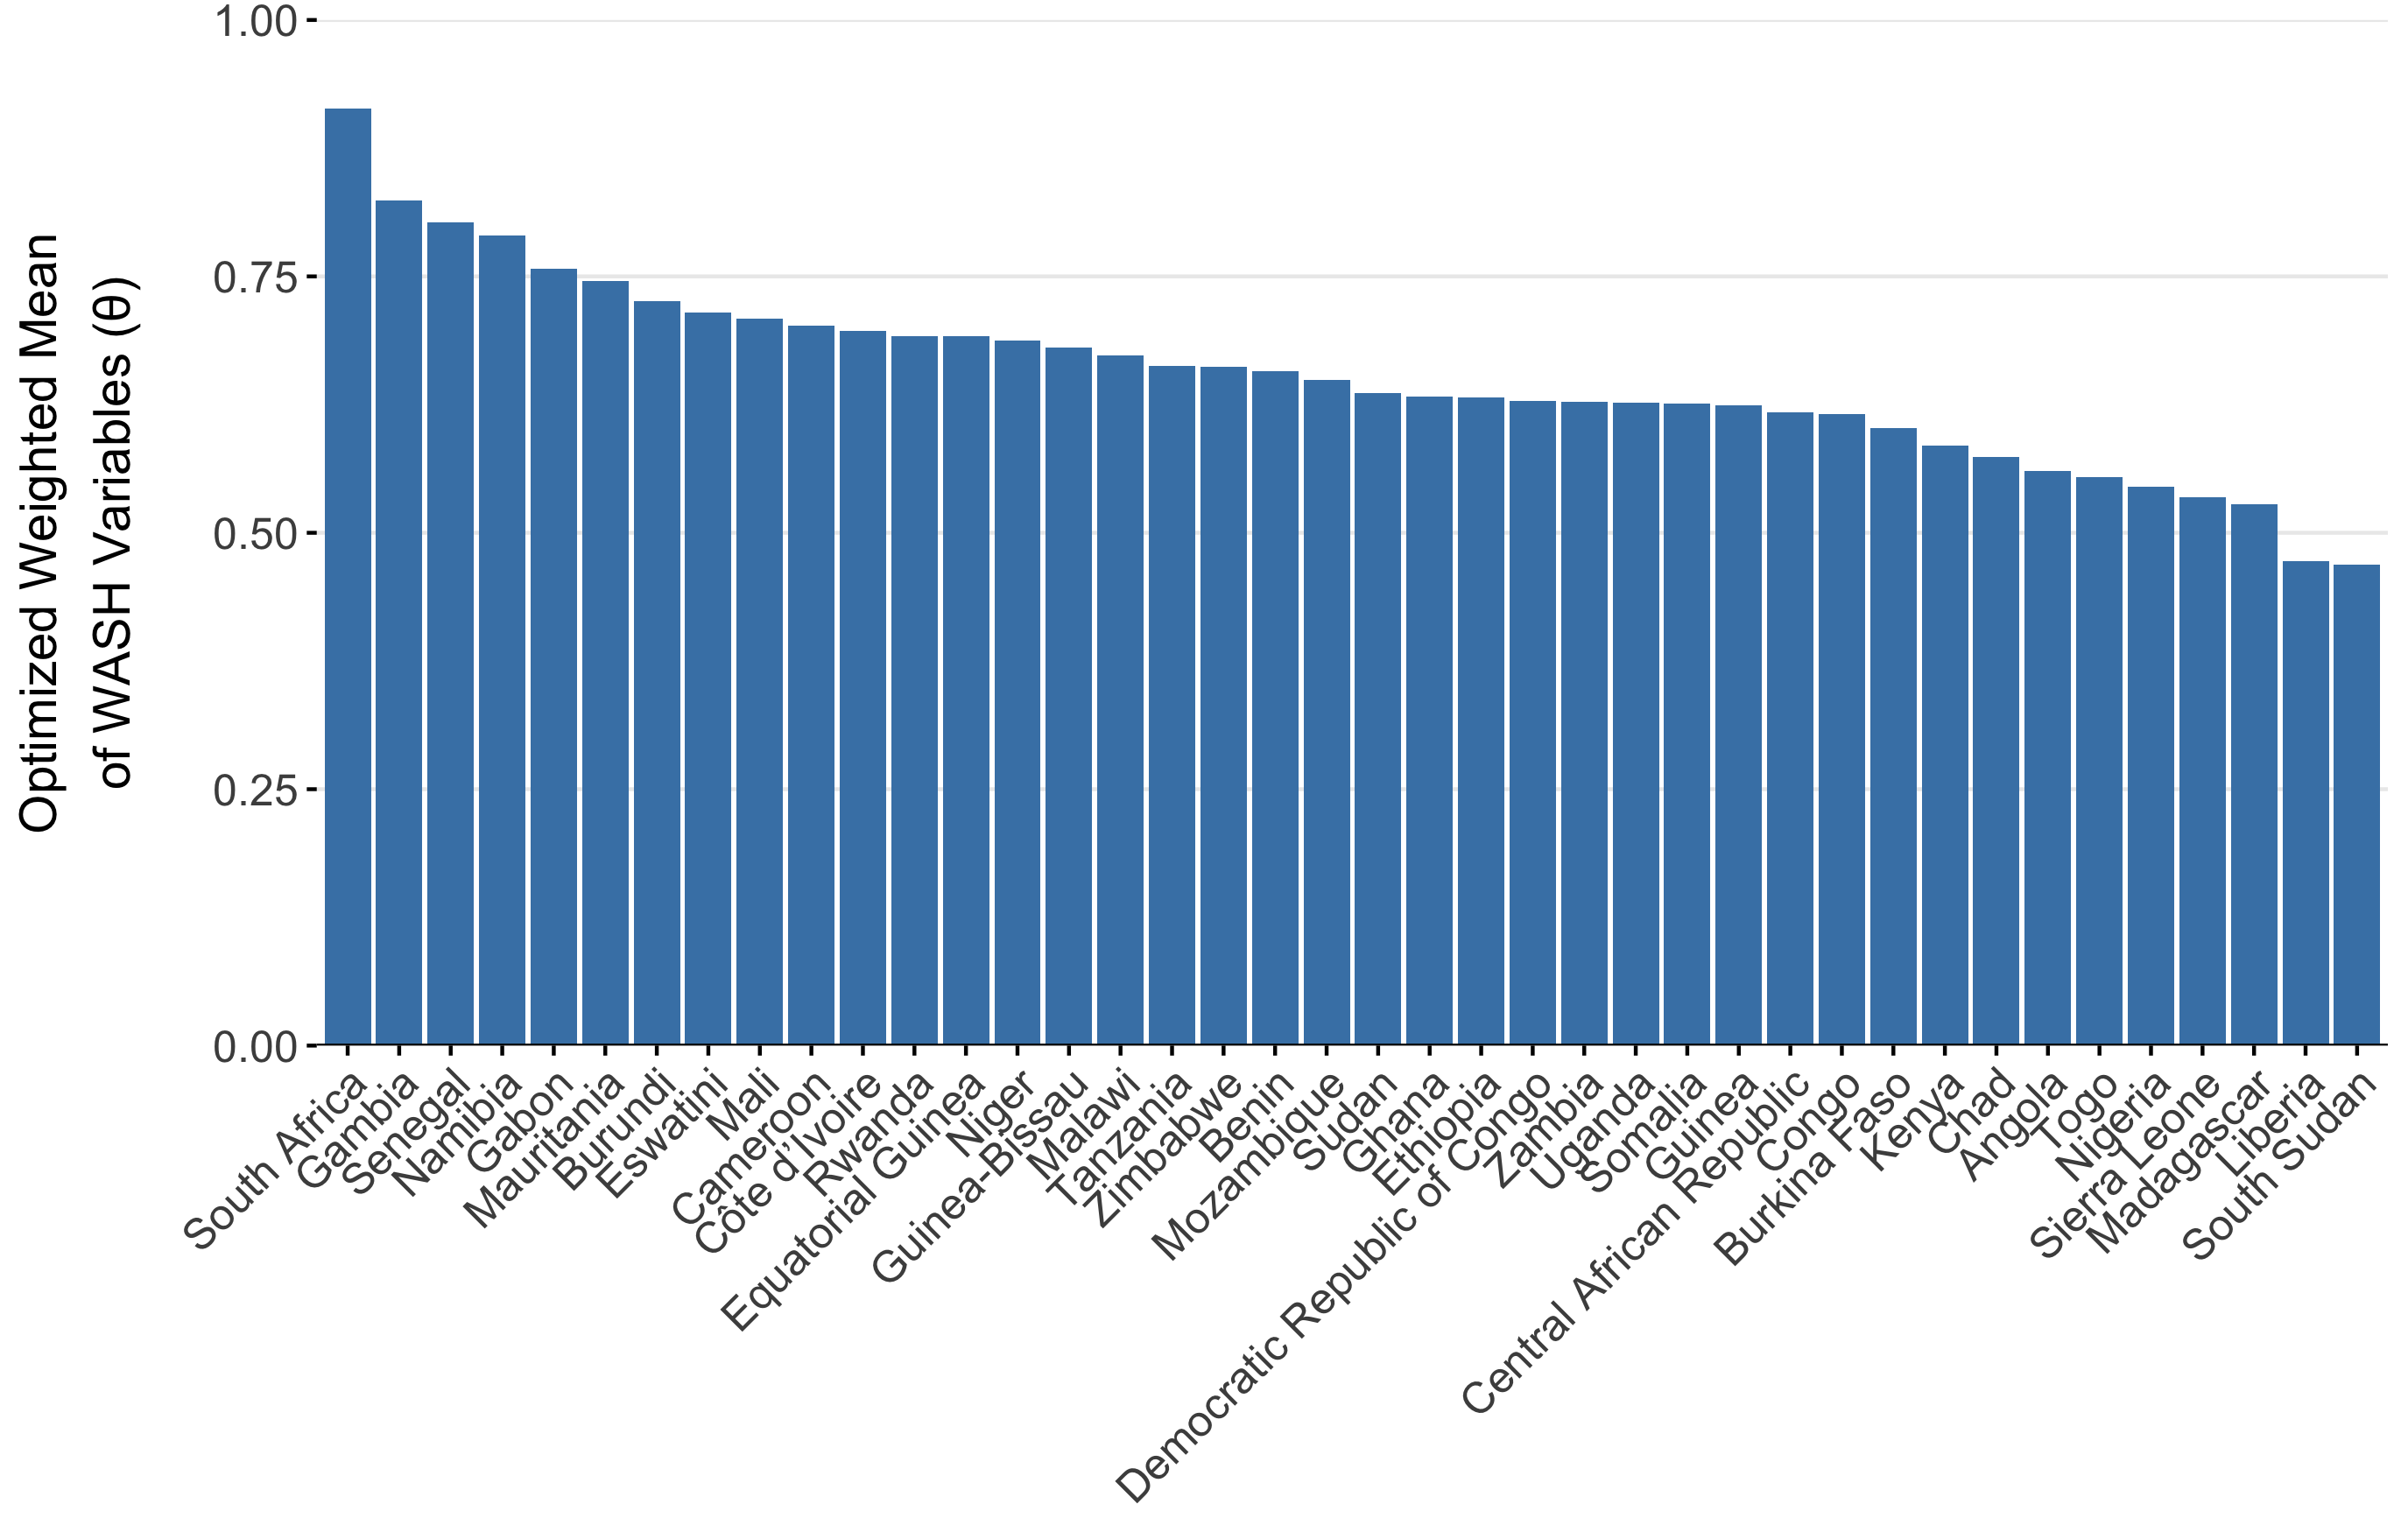
\includegraphics[width=1\linewidth]{figures/wash_index_by_country} 

}

\caption{The optimized weighted mean of WASH variables for AFRO countries. Countries labeled in orange denote countries with an imputed weighted mean WASH variable. Imputed values are the weighted mean from the 3 most similar countries.}\label{fig:wash-country}
\end{figure}

\section{Immune dynamics}\label{immune-dynamics}

Aside from the current number of infections, population susceptibility is one of the key factors influencing the spread of cholera. Further, since immunity from both vaccination and natural infection provides long-lasting protection, it's crucial to quantify not only the incidence of cholera but also the number of past vaccinations. Additionally, we need to estimate how many individuals with immunity remain in the population at any given time step in the model.

To achieve this, we estimate the vaccination rate over time (\(\nu_{jt}\)) based on historical vaccination campaigns and incorporate a model of vaccine effectiveness (\(\phi\)) and immune decay post-vaccination (\(\omega\)) to estimate the current number of individuals with vaccine-derived immunity. We also account for the immune decay rate from natural infection (\(\varepsilon\)), which is generally considered to last longer than immunity from vaccination.

\subsection{Estimating Vaccination Rates}\label{estimating-vaccination-rates}

To estimate the past and current vaccination rates, we sourced data on reported OCV vaccinations from the WHO \href{https://www.who.int/groups/icg}{International Coordinating Group} (ICG) \href{https://app.powerbi.com/view?r=eyJrIjoiYmFmZTBmM2EtYWM3Mi00NWYwLTg3YjgtN2Q0MjM5ZmE1ZjFkIiwidCI6ImY2MTBjMGI3LWJkMjQtNGIzOS04MTBiLTNkYzI4MGFmYjU5MCIsImMiOjh9}{Cholera vaccine dashboard}. This resource lists all reactive OCV campaigns conducted from 2016 to the present, with approximately 103 million OCV doses shipped to Sub-Saharan African (SSA) countries as of October 9, 2024. However, these data only capture reactive vaccinations in emergency settings and do not include preventive campaigns organized by GAVI and in-country partners.

\emph{As a result, our current estimates of the OCV vaccination rate likely underestimate total OCV coverage. We are working to expand our data sources to better reflect the full number of OCV doses distributed in SSA and will update the results here as soon as these are available.}

To translate the reported number of OCV doses into the model parameter \(\nu_{jt}\), we take the number of doses shipped and the reported start date of the vaccination campaign, distributing the doses over subsequent days according to a maximum daily vaccination rate. Therefore, the vaccination rate \(\nu_t\) is not an estimated quantity, it is defined by the reported number of OCV doses administered with a assumption about the daily rate of distribution for an OCV campaign:

\[
\nu_{jt} = f\big(\text{reported OCV doses distributed}_{jt} \ | \ \text{daily distribution rate}\big).    
\]

See Figure \ref{fig:vaccination-example} for an example of OCV distribution using a maximum daily vaccination rate of 100,000. The resulting time series for each country is shown in Figure \ref{fig:vaccination-countries}, with current totals based on the WHO ICG data displayed in Figure \ref{fig:vaccination-maps}.

\begin{figure}

{\centering 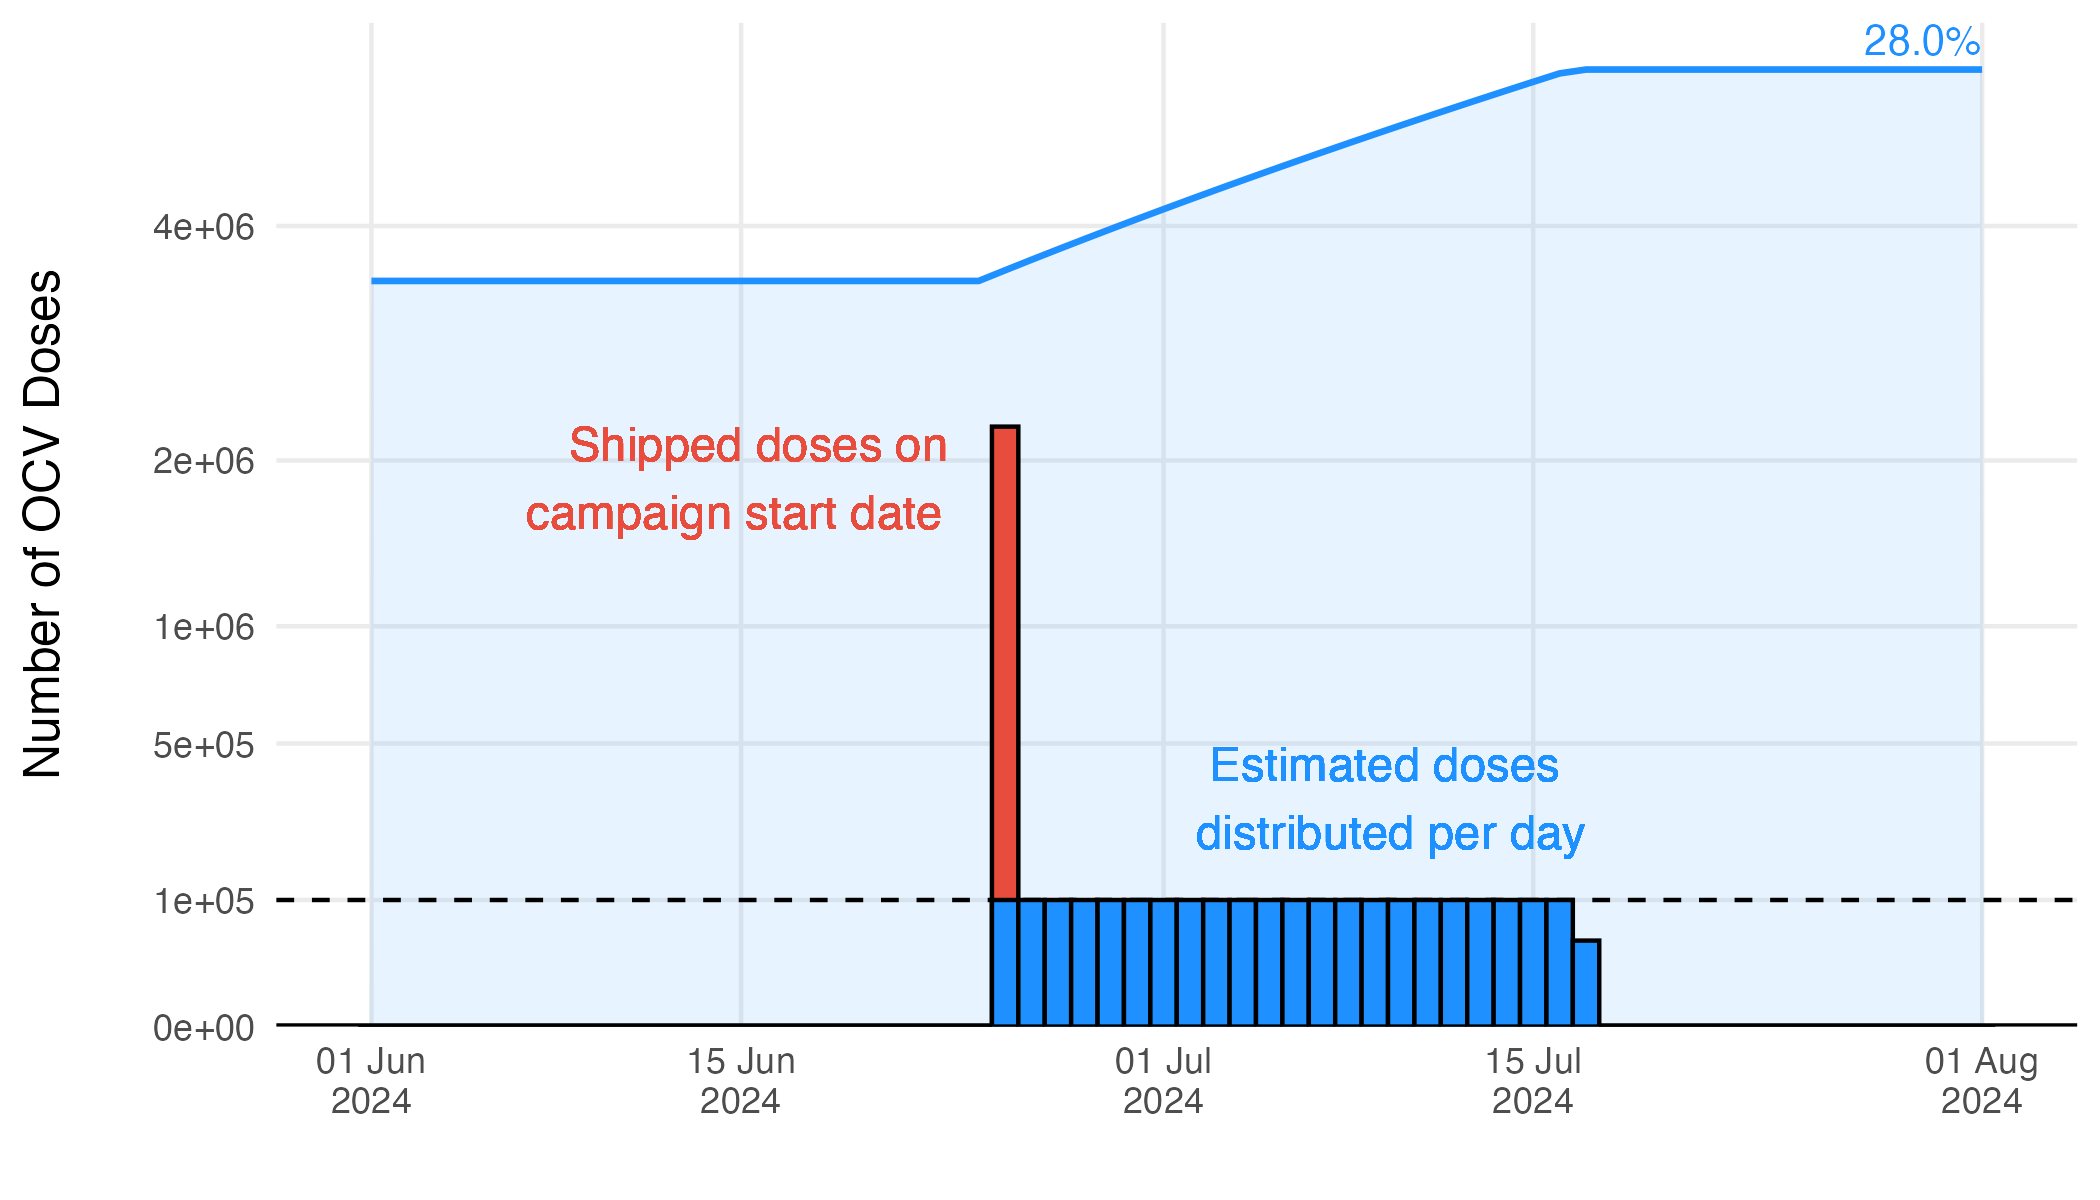
\includegraphics[width=1\linewidth]{figures/vaccination_example_ZMB} 

}

\caption{Example of the estimated vaccination rate during an OCV campaign.}\label{fig:vaccination-example}
\end{figure}

\begin{figure}

{\centering 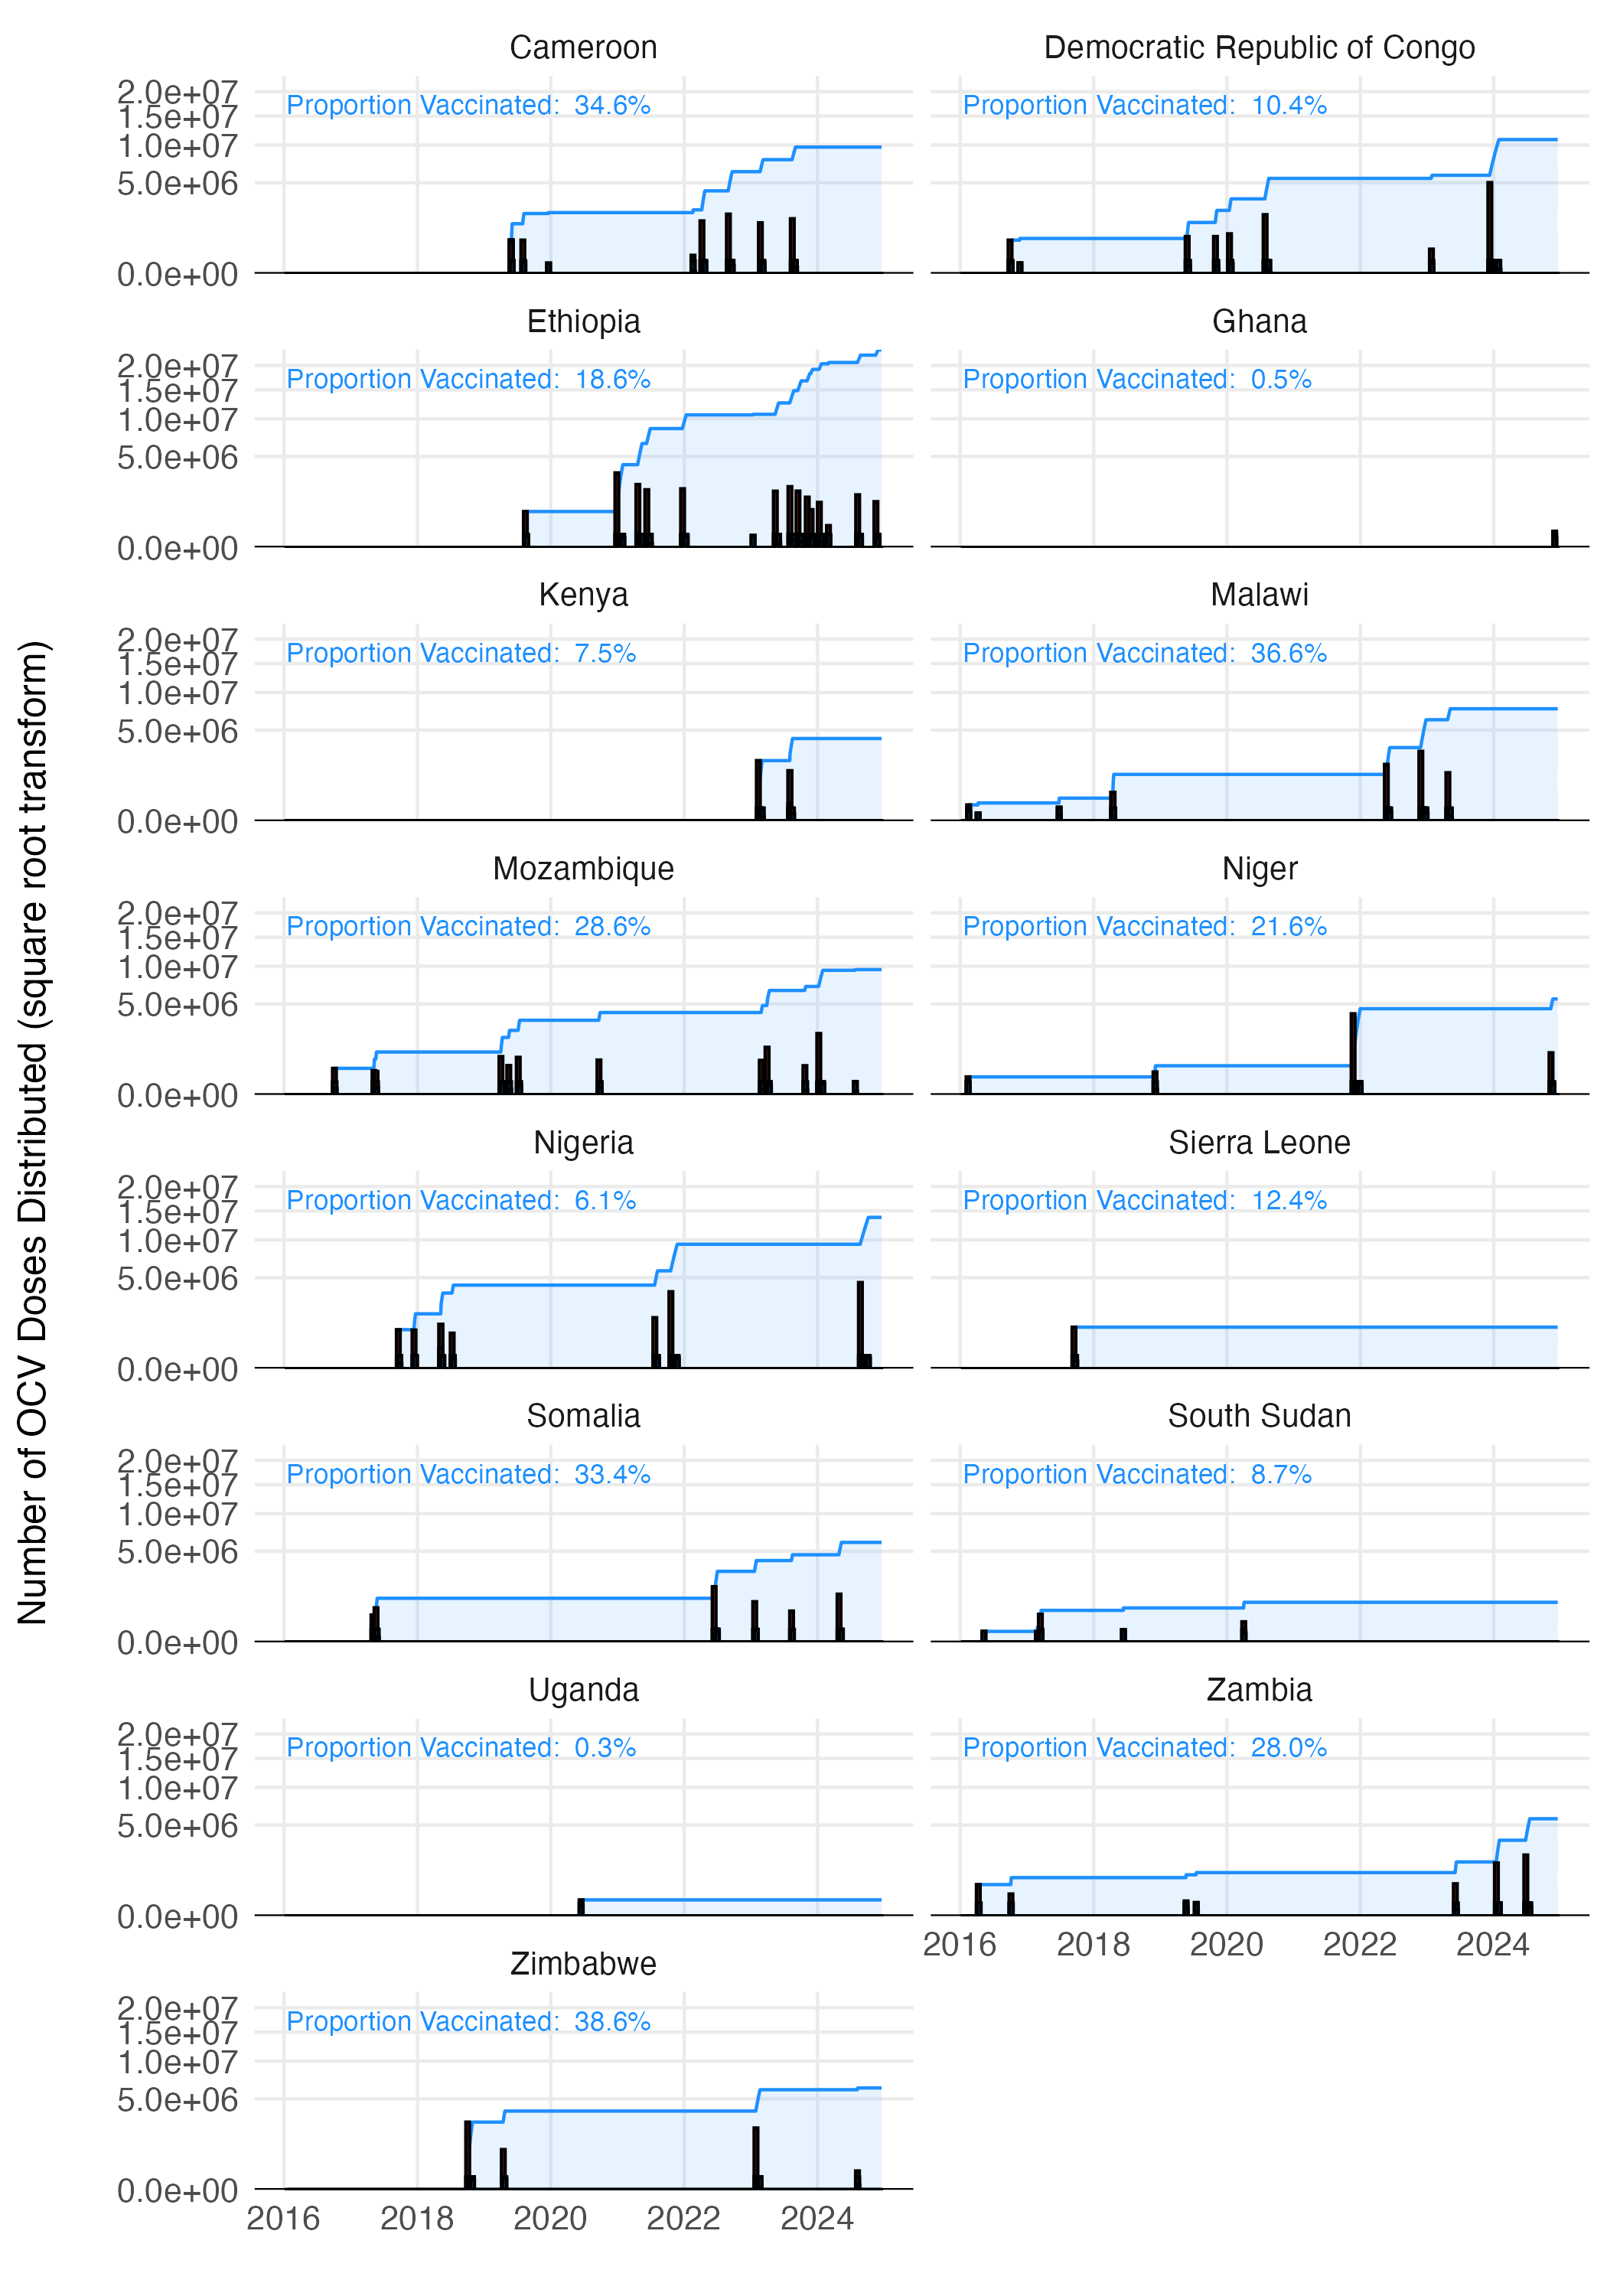
\includegraphics[width=1\linewidth]{figures/vaccination_by_country} 

}

\caption{The estimated vaccination coverage across all countries with reported vaccination data one the WHO ICG dashboard.}\label{fig:vaccination-countries}
\end{figure}

\begin{figure}

{\centering 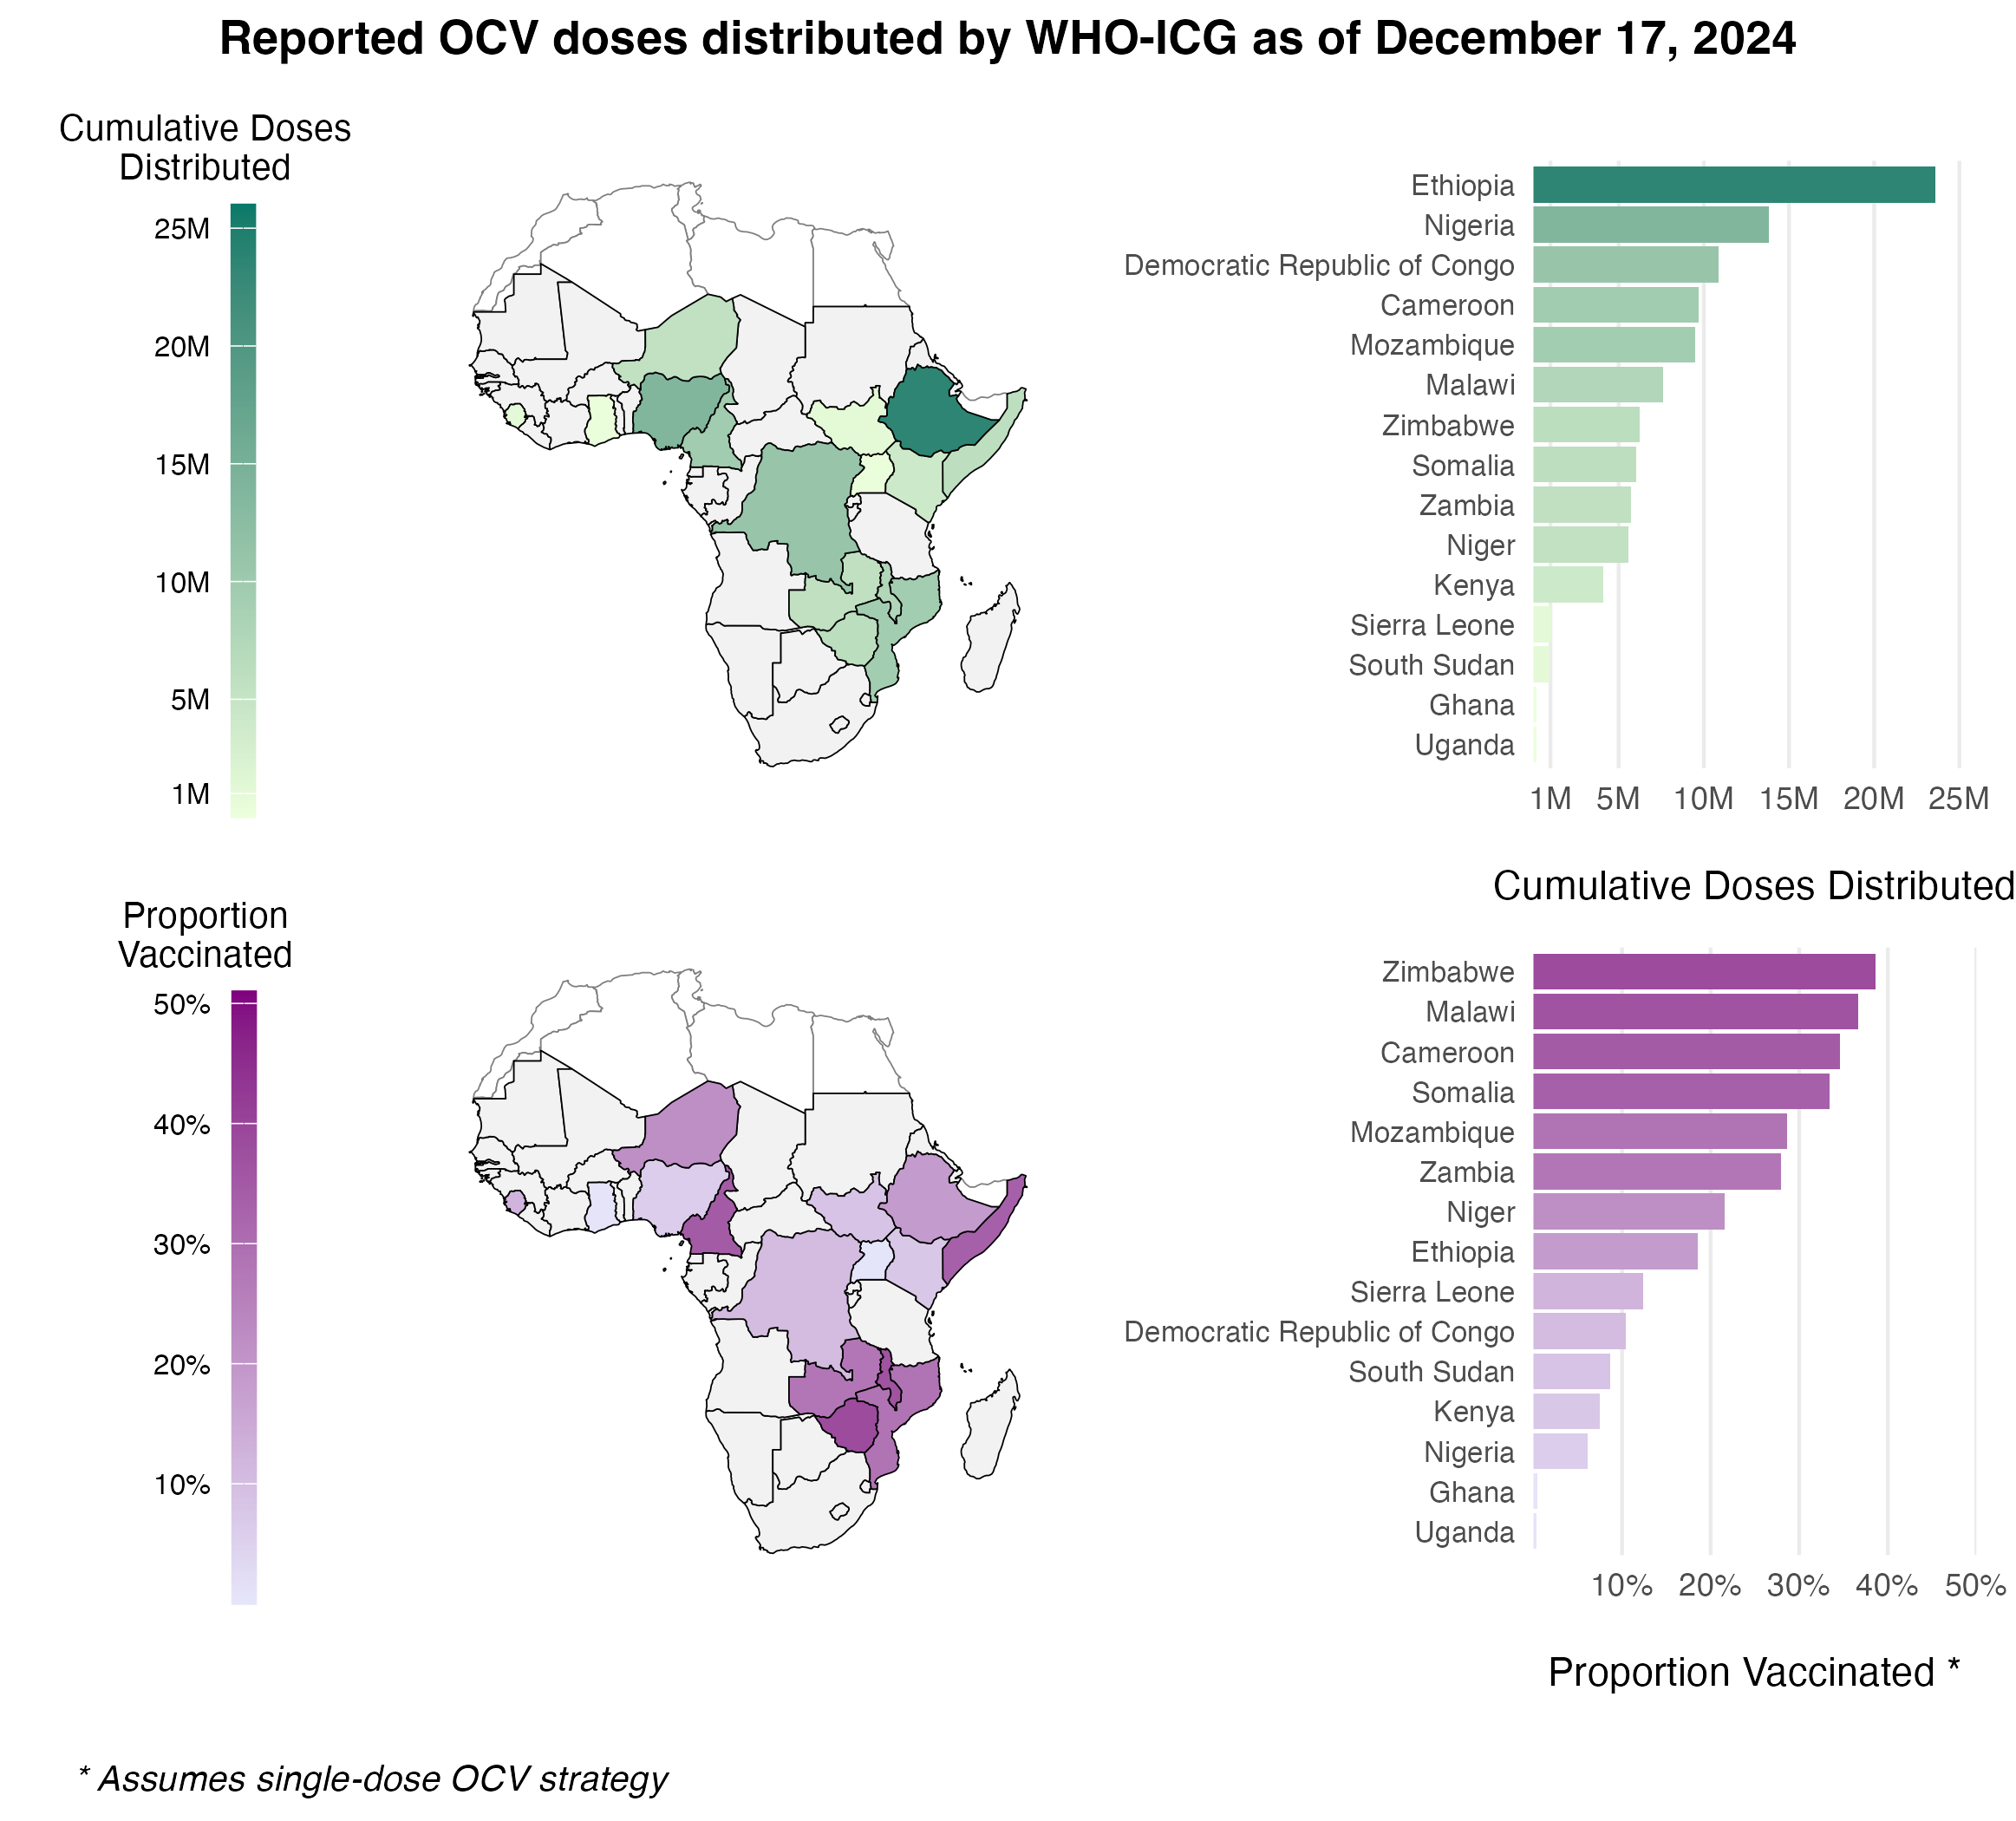
\includegraphics[width=1\linewidth]{figures/vaccination_maps} 

}

\caption{The total cumulative number of OCV doses distributed through the WHO ICG from 2016 to present day.}\label{fig:vaccination-maps}
\end{figure}

\subsection{Immunity from vaccination}\label{immunity-from-vaccination}

The impacts of Oral Cholera Vaccine (OCV) campaigns is incorporated into the model through the Vaccinated compartment (V). The rate that individuals are effectively vaccinated is defined as \(\phi\nu_t\), where \(\nu_t\) is the number of OCV doses administered in location \(j\) at time \(t\) and \(\phi\) is the estimated vaccine effectiveness. The vaccination rate \(\nu_{jt}\) is not an estimated quantity. Rather, it is directly defined by the reported number of OCV doses administered as described above. Note that there is just one vaccinated compartment at this time, though future model versions may include \(V_1\) an \(V_2\) compartments to explore two dose vaccination strategies or to emulate more complex waning patterns.

The evidence for waning immunity comes from 4 cohort studies (Table \ref{tab:effectiveness-papers}) from Bangladesh (\href{https://www.nejm.org/doi/full/10.1056/NEJMoa1510330}{Qadri et al 2016} and \href{https://www.thelancet.com/journals/laninf/article/PIIS1473-3099(18)30108-7/fulltext}{2018}), South Sudan (\href{https://www.thelancet.com/journals/langlo/article/PIIS2214-109X(16)30211-X/fulltext}{Azman et al 2016}), and Democratic Republic of Congo (\href{https://www.thelancet.com/journals/laninf/article/PIIS1473-3099(23)00742-9/fulltext}{Malembaka et al 2024}).

\begin{table}

\caption{\label{tab:effectiveness-papers}Summary of Effectiveness Data}
\centering
\begin{tabular}[t]{r|r|r|r|r|r|l}
\hline
Effectiveness & Upper CI & Lower CI & Day (midpoint) & Day (min) & Day (max) & Source\\
\hline
60.0 & 0.873 & 0.990 & 0.702 & NA & NA & Azman et al (2016)\\
\hline
93.5 & 0.400 & 0.600 & 0.110 & 7 & 180 & Qadri et al (2016)\\
\hline
368.5 & 0.390 & 0.520 & 0.230 & 7 & 730 & Qadri et al (2018)\\
\hline
435.0 & 0.527 & 0.674 & 0.314 & 360 & 510 & Malembaka et al (2024)\\
\hline
900.0 & 0.447 & 0.594 & 0.248 & 720 & 1080 & Malembaka et al (2024)\\
\hline
\end{tabular}
\end{table}

We estimated vaccine effectiveness and waning immunity by fitting an exponential decay model to the reported effectiveness of one dose OCV in these studies using the following formulation:

\begin{equation} 
\text{Proportion immune}\ t \ \text{days after vaccination} = \phi \times (1 - \omega) ^ {t-t_{\text{vaccination}}}
\label{eq:omega}
\end{equation}

Where \(\phi\) is the effectiveness of one dose OCV, and the based on this specification, it is also the initial proportion immune directly after vaccination. The decay rate parameter \(\omega\) is the rate at which initial vaccine derived immunity decays per day post vaccination, and \(t\) and \(t_{\text{vaccination}}\) are the time (in days) the function is evaluated at and the time of vaccination respectively. When we fitted the model to the data from the cohort studies shown in Table (\ref{tab:effectiveness-papers}) we found that \(\omega = 0.00057\) (\(0-0.0019\) 95\% CI), which gives a mean estimate of 4.8 years for vaccine derived immune duration with unreasonably large confidence intervals (1.4 years to infinite immunity). However, the point estimate of 4.8 years is consistent with anecdotes that one dose OCV is effective for up to at least 3 years.

The wide confidence intervals are likely due to the wide range of reported estimates for proportion immune after a short duration in the 7--90 days range (\href{https://www.thelancet.com/journals/langlo/article/PIIS2214-109X(16)30211-X/fulltext}{Azman et al 2016} and \href{https://www.nejm.org/doi/full/10.1056/NEJMoa1510330}{Qadri et al 2016}). Therefore, we chose to use the point estimate of \(\omega\) and incorporate uncertainty based on the initial proportion immune (i.e.~vaccine effectiveness \(\phi\)) shortly after vaccination. Using the decay model in Equation \eqref{eq:omega} we estimated \(\phi\) to be \(0.64\) (\(0.32-0.96\) 95\% CI). We then fit a Beta distribution to the quantiles of \(\phi\) by minimizing the sums of squares using the Nelder-Mead optimization algorithm to render the following distribution (shown in Figure \ref{fig:effectiveness}B):

\begin{equation} 
\phi \sim \text{Beta}(4.57, 2.41).
\label{eq:effectiveness}
\end{equation}

\begin{figure}

{\centering 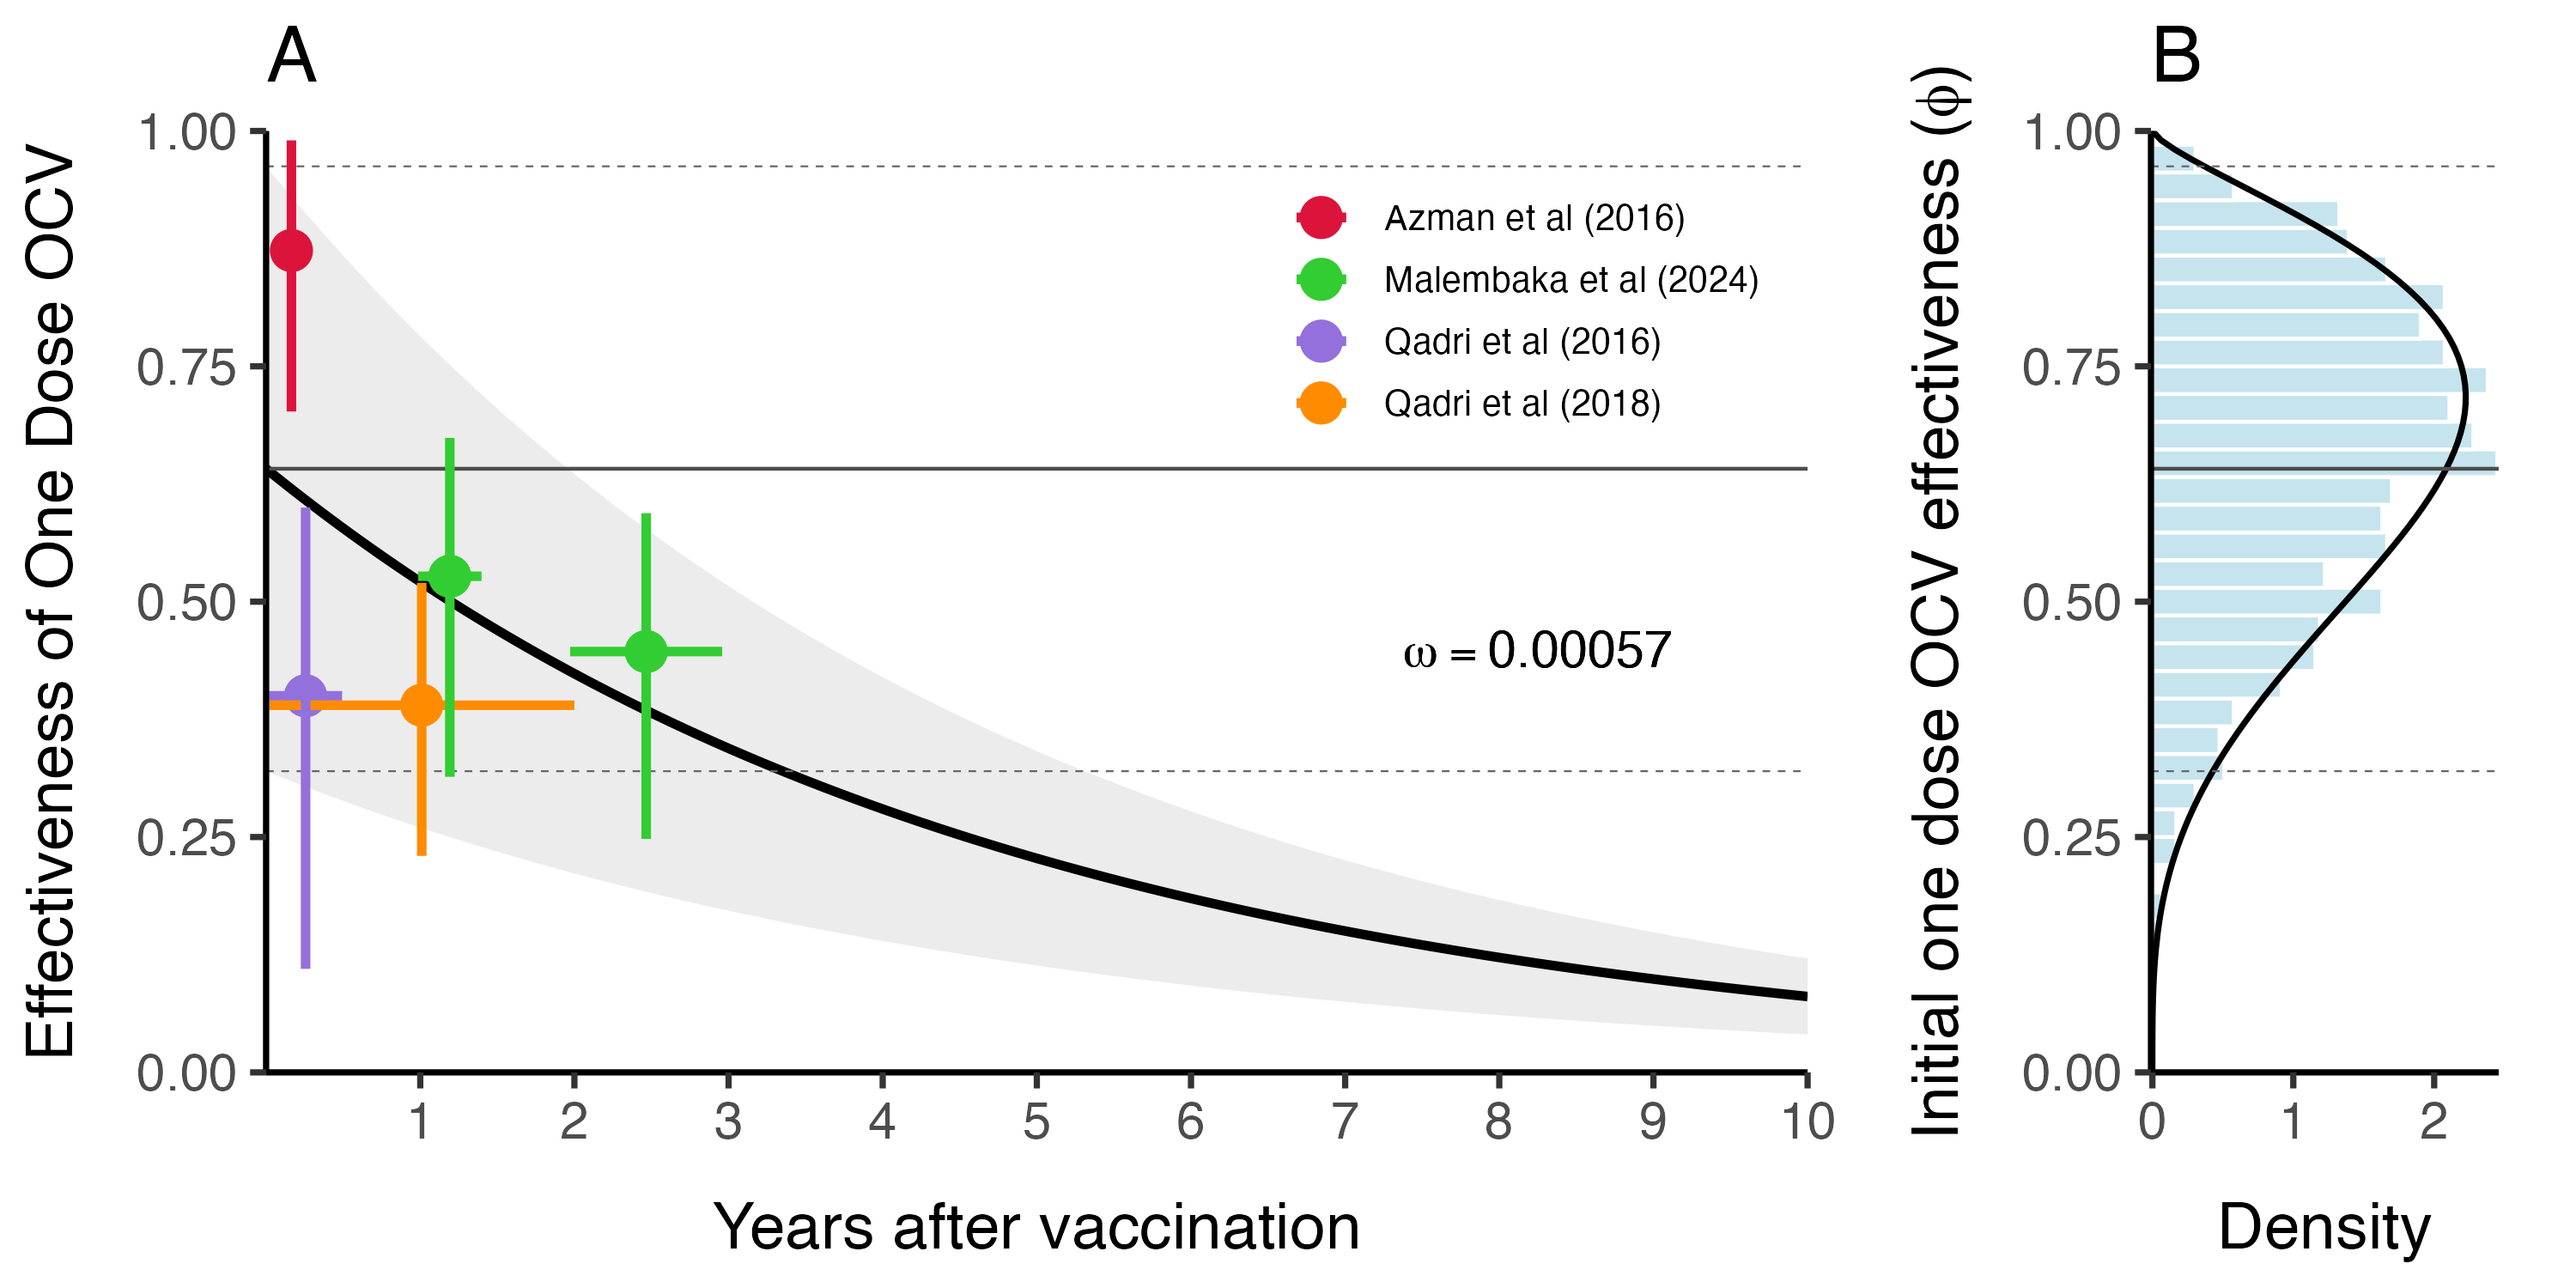
\includegraphics[width=1.02\linewidth]{figures/vaccine_effectiveness} 

}

\caption{This is vaccine effectiveness}\label{fig:effectiveness}
\end{figure}

\subsection{Immunity from natural infection}\label{immunity-from-natural-infection}

The duration of immunity after a natural infection is likely to be longer lasting than that from vaccination with OCV (especially given the current one dose strategy). As in most SIR-type models, the rate at which individuals leave the Recovered compartment is governed by the immune decay parameter \(\varepsilon\). We estimated the durability of immunity from natural infection based on two cohort studies and fit the following exponential decay model to estimate the rate of immunity decay over time:

\[
\text{Proportion immune}\ t \ \text{days after infection} = 0.99 \times (1 - \varepsilon) ^ {t-t_{\text{infection}}}
\]
Where we make the necessary and simplifying assumption that within 0--90 days after natural infection with \emph{V. cholerae}, individuals are 95--99\% immune. We fit this model to reported data from \href{https://doi.org/10.1093/infdis/jir416}{Ali et al (2011)} and \href{https://www.sciencedirect.com/science/article/pii/0140673691902076}{Clemens et al (1991)} (see Table \ref{tab:immunity-sources}).

\begin{table}

\caption{\label{tab:immunity-sources}Sources for the duration of immunity fro natural infection.}
\centering
\begin{tabular}[t]{r|r|r|r|l}
\hline
Day & Effectiveness & Upper CI & Lower CI & Source\\
\hline
90 & 0.95 & 0.95 & 0.95 & Assumption\\
\hline
1080 & 0.65 & 0.81 & 0.37 & [Ali et al (2011)](https://doi.org/10.1093/infdis/jir416)\\
\hline
1260 & 0.61 & 0.81 & 0.21 & [Clemens et al (1991)](https://www.sciencedirect.com/science/article/pii/0140673691902076)\\
\hline
\end{tabular}
\end{table}

We estimated the mean immune decay to be \(\bar\varepsilon = 3.9 \times 10^{-4}\) (\(1.7 \times 10^{-4}-1.03 \times 10^{-3}\) 95\% CI) which is equivalent to an immune duration of \(7.21\) years (\(2.66-16.1\) years 95\% CI) as shown in Figure \ref{fig:immune-decay}A. This is slightly longer than previous modeling work estimating the duration of immunity to be \textasciitilde5 years (\href{https://www.nature.com/articles/nature07084}{King et al 2008}). Uncertainty around \(\varepsilon\) in the model is then represented by a Log-Normal distribution as shown in Figure \ref{fig:immune-decay}B:

\[
\varepsilon \sim \text{Lognormal}(\bar\varepsilon+\frac{\sigma^2}{2}, 0.25)
\]

\begin{figure}

{\centering 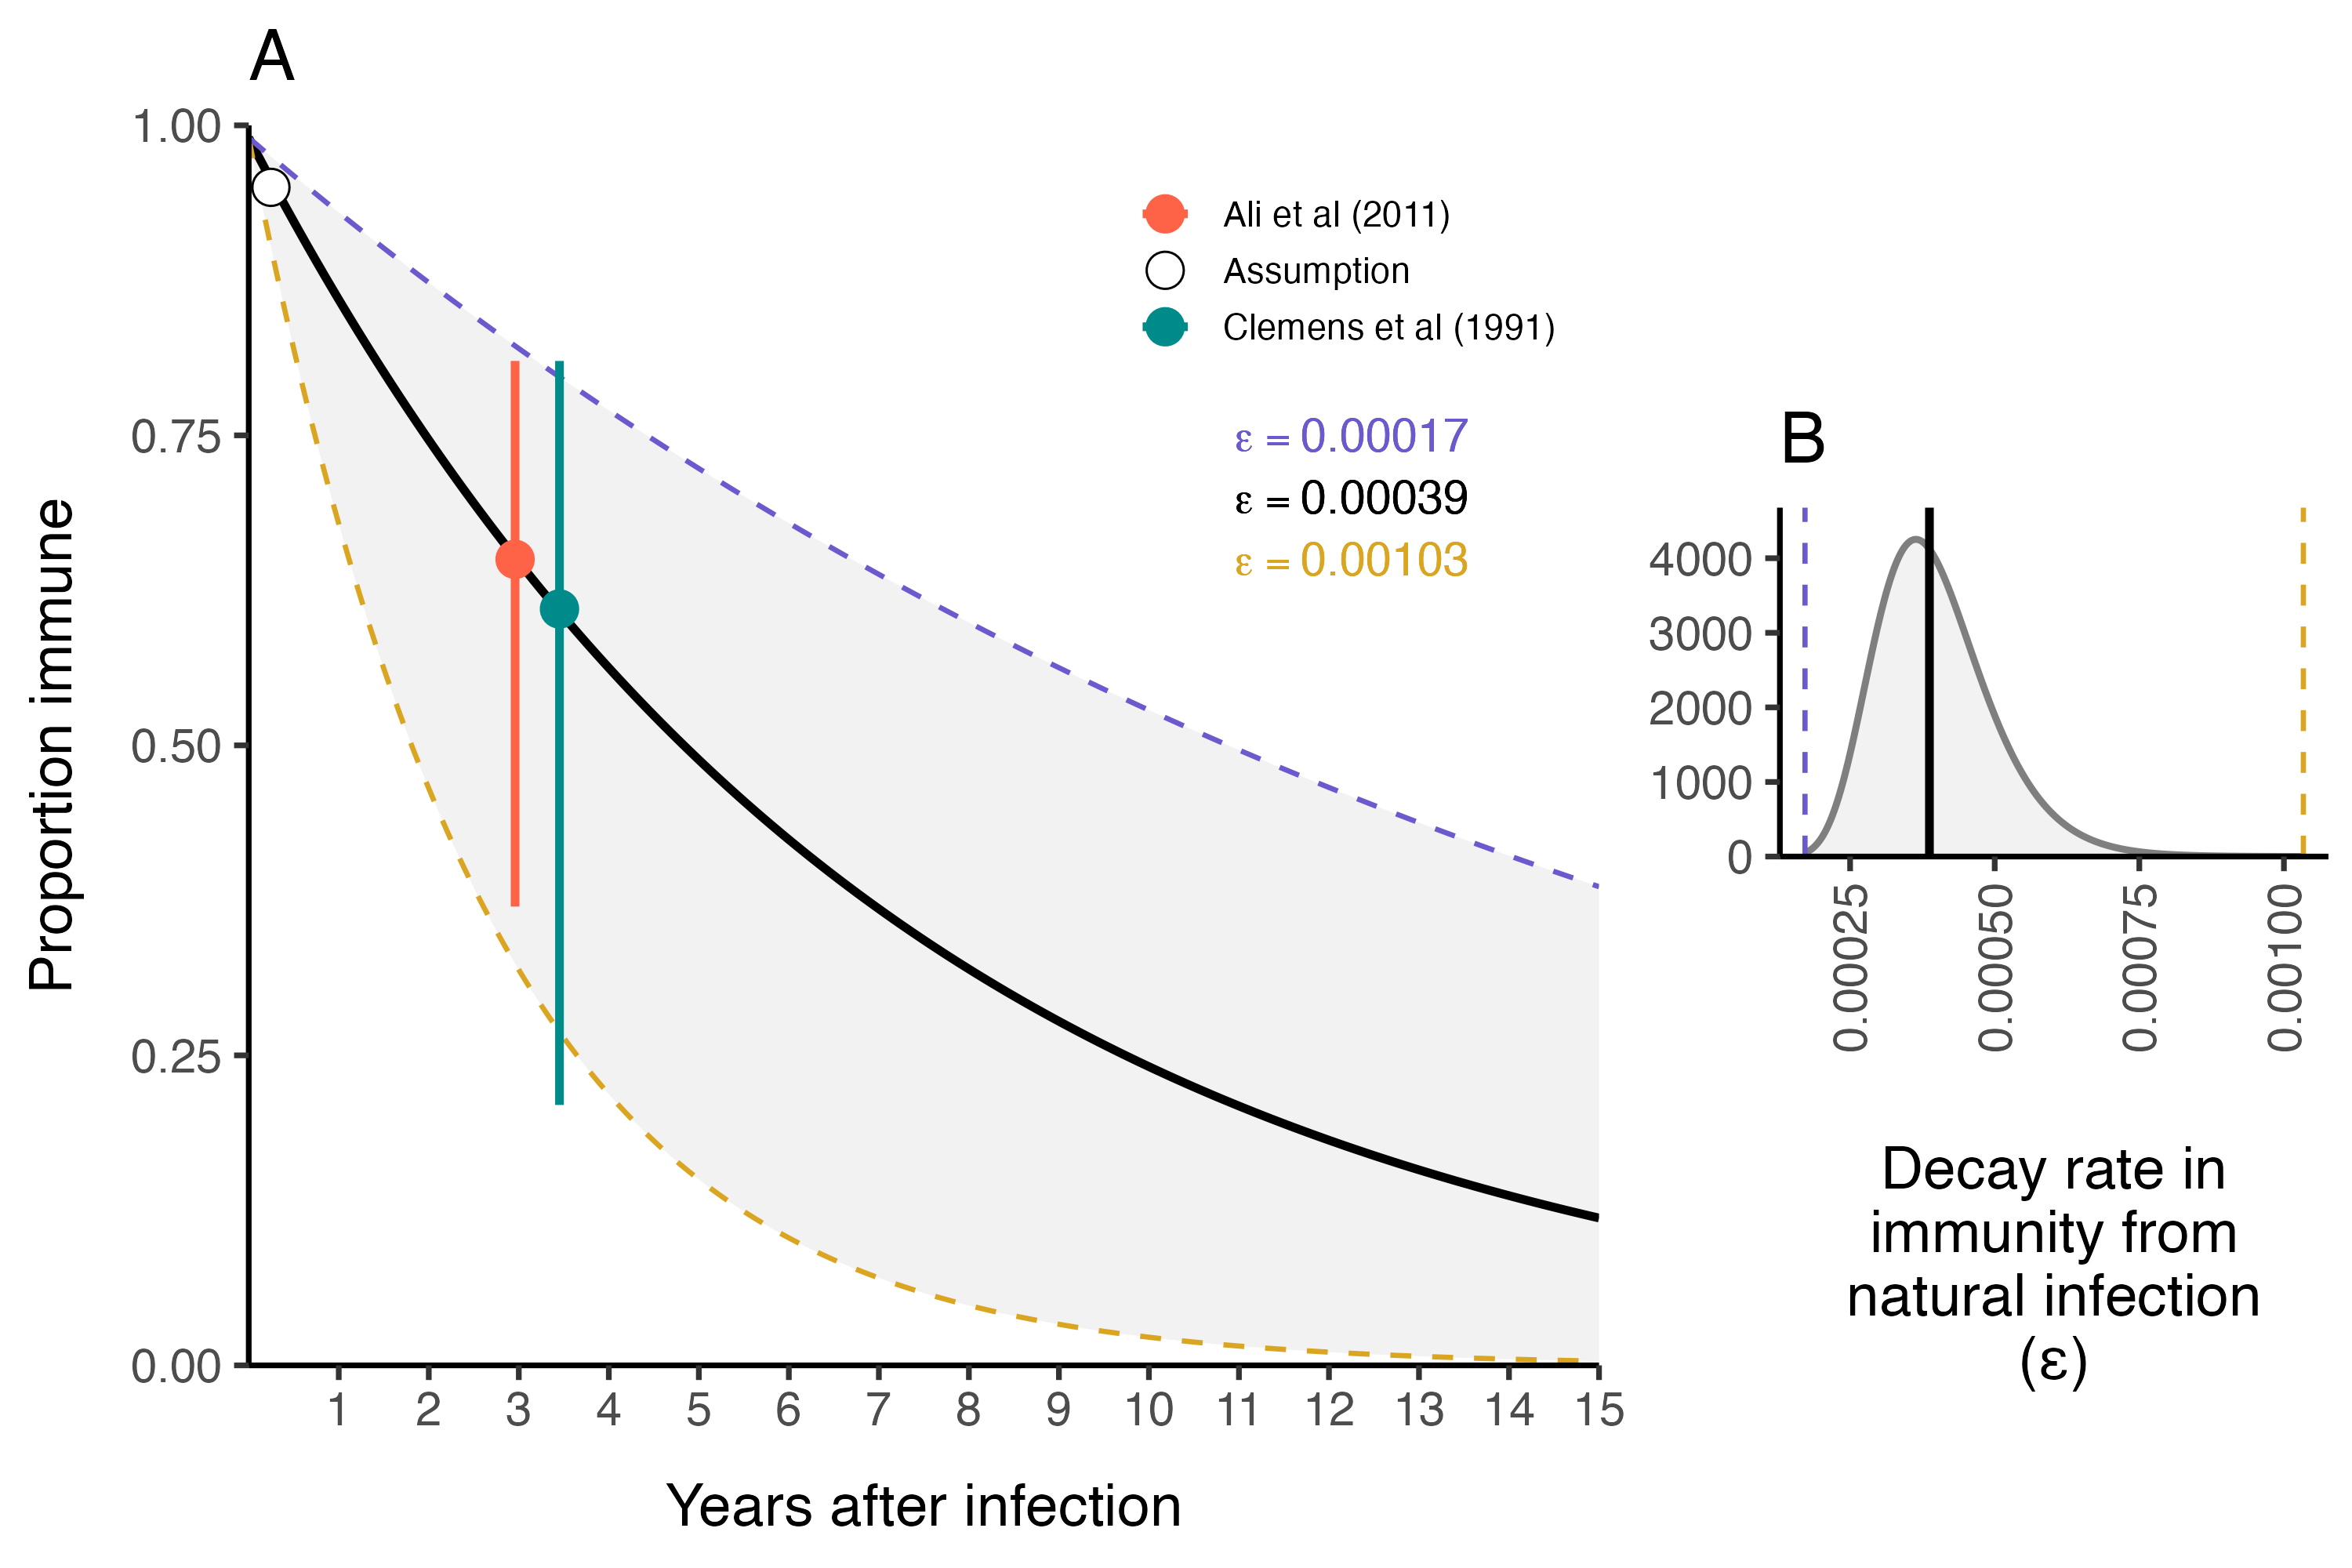
\includegraphics[width=1\linewidth]{figures/immune_decay} 

}

\caption{The duration of immunity after natural infection with *V. cholerae*.}\label{fig:immune-decay}
\end{figure}

\section{Spatial dynamics}\label{spatial-dynamics}

The parameters in the model diagram in Figure \ref{fig:diagram} that have a \(jt\) subscript denote the spatial structure of the model. Each country is modeled as an independent metapopulation that is connected to all others via the spatial force of infection \(\Lambda_{jt}\) which moves contagion among metapopulations according to the connectivity provided by parameters \(\tau_i\) (the probability departure) and \(\pi_{ij}\) (the probability of diffusion to destination \(j\)). Both parameters are estimated using the departure-diffusion model below which is fitted to average weekly air traffic volume between all of the 41 countries included in the MOSAIC framework (Figure \ref{fig:mobility-data}).

\begin{figure}

{\centering 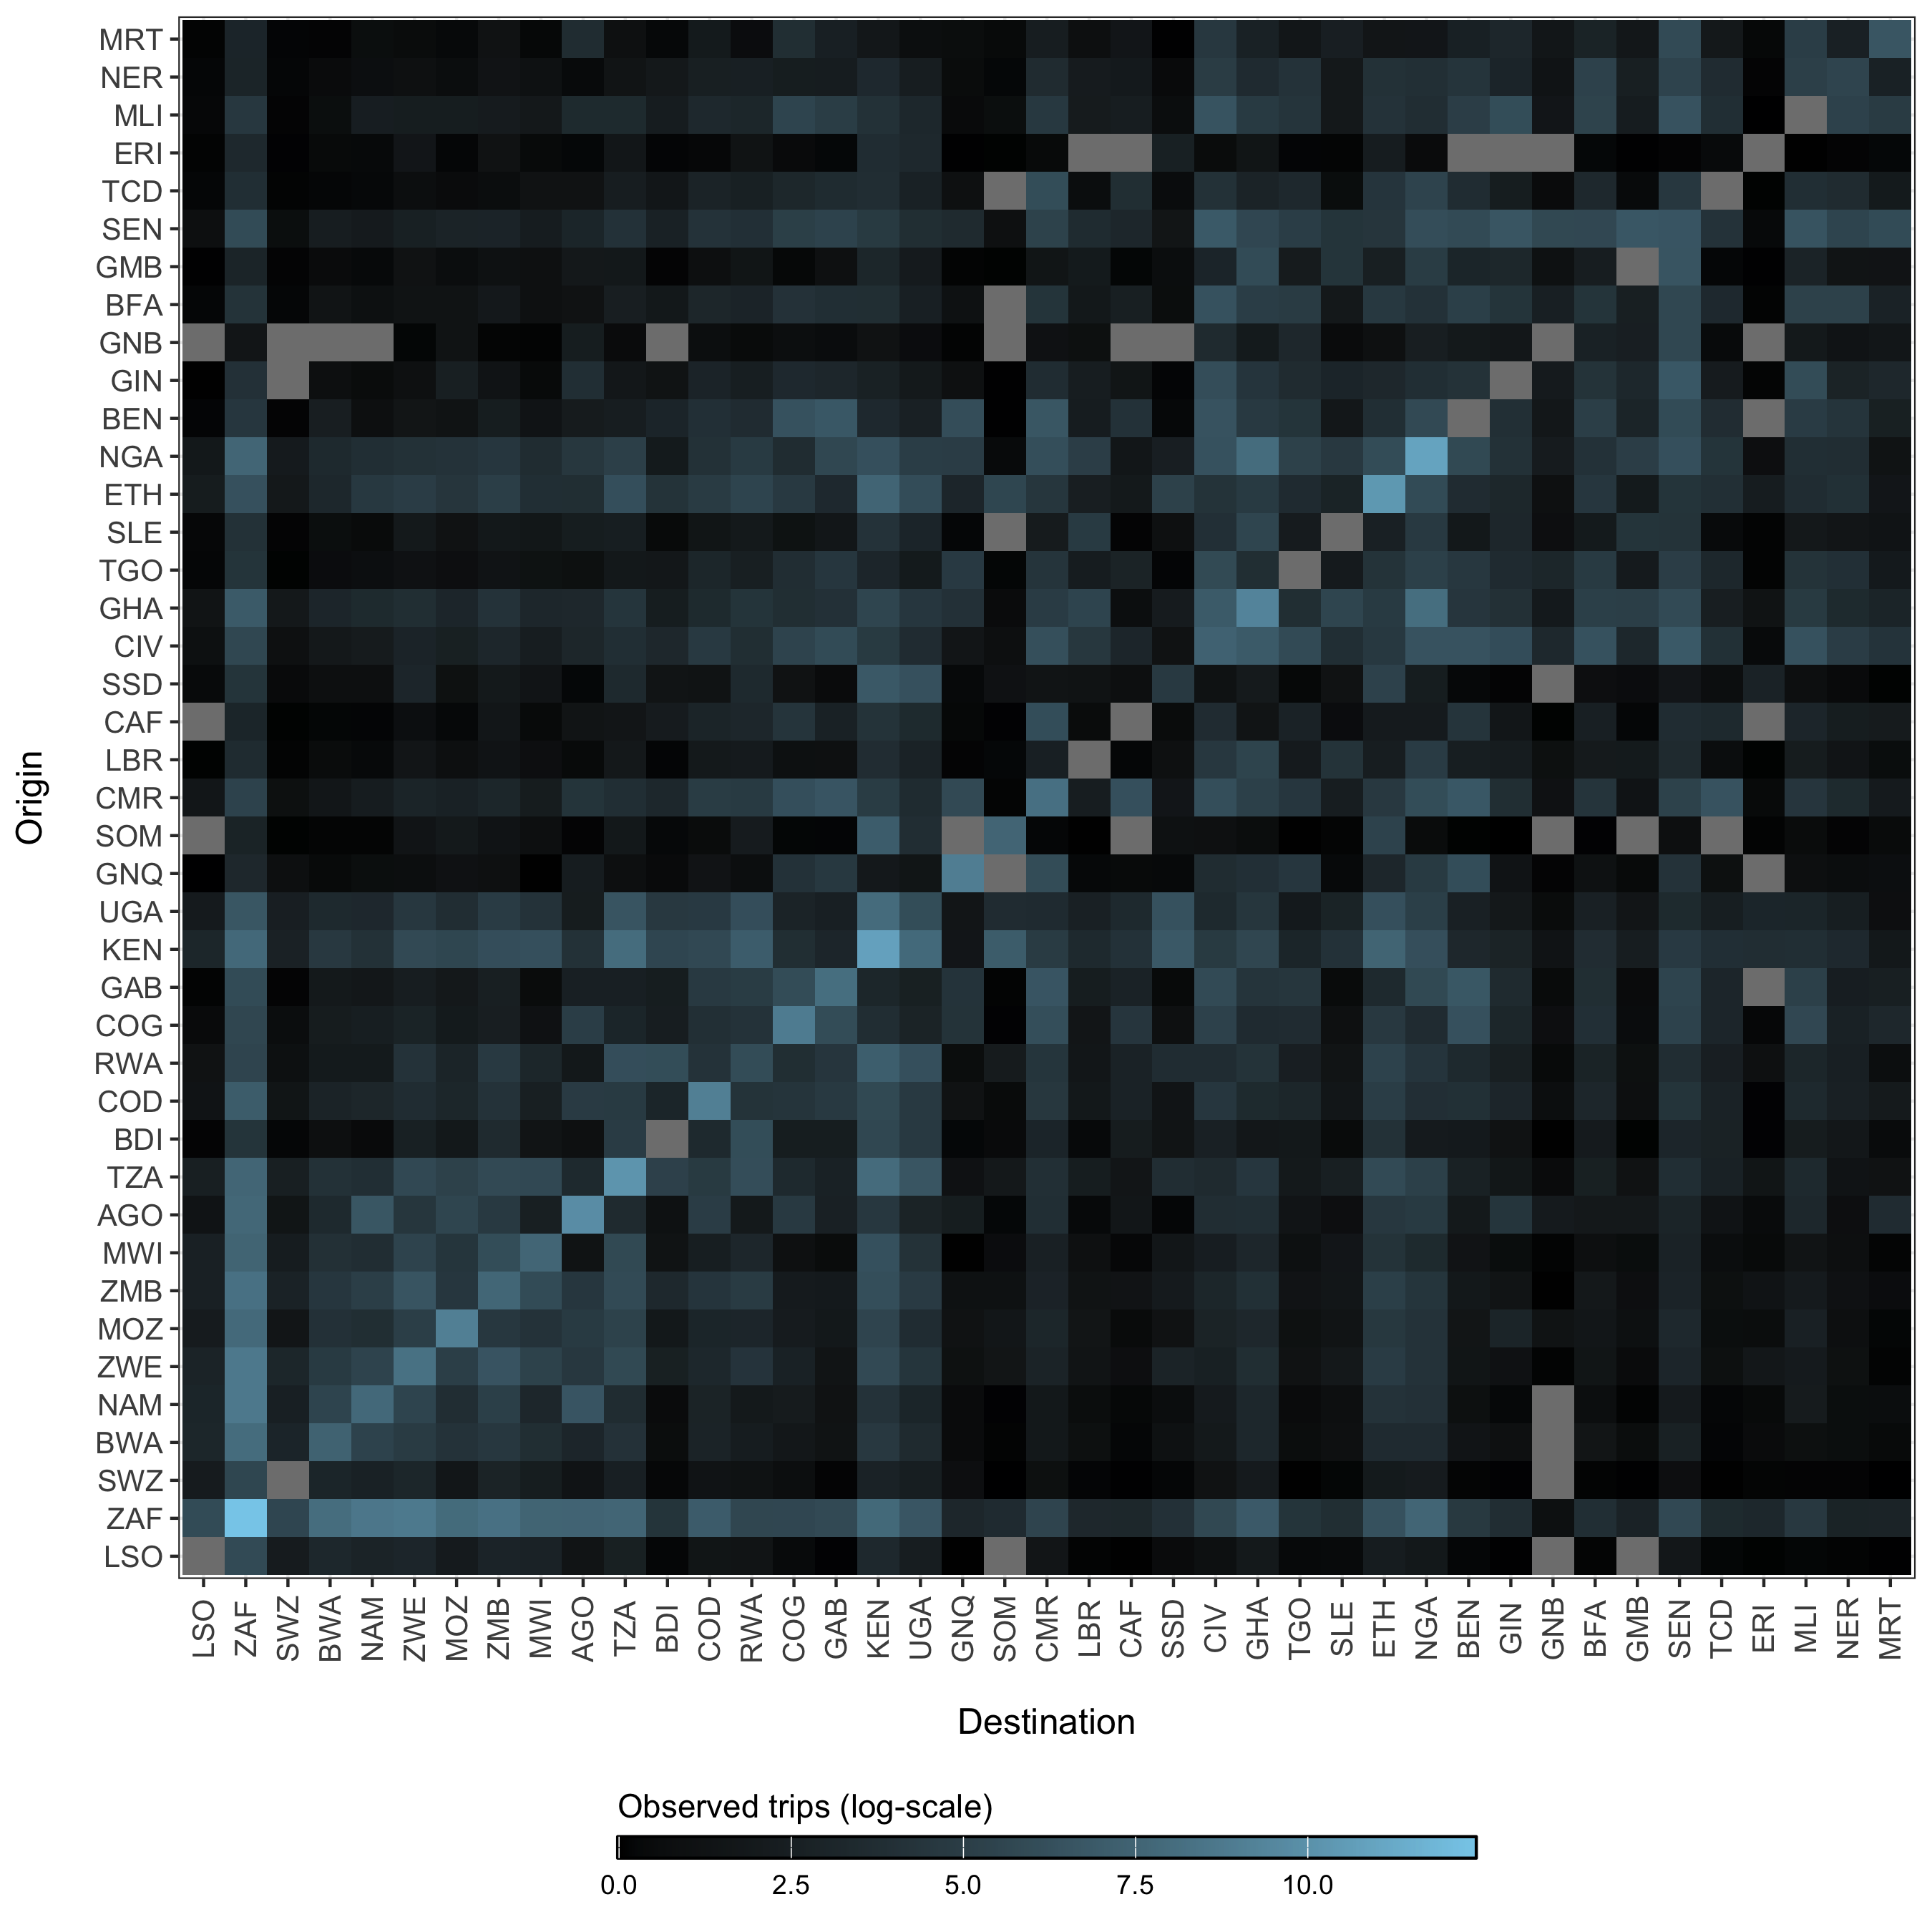
\includegraphics[width=1\linewidth]{figures/mobility_flight_data} 

}

\caption{The average number of air passengers per week in 2017 among all countries.}\label{fig:mobility-data}
\end{figure}
\begin{figure}

{\centering 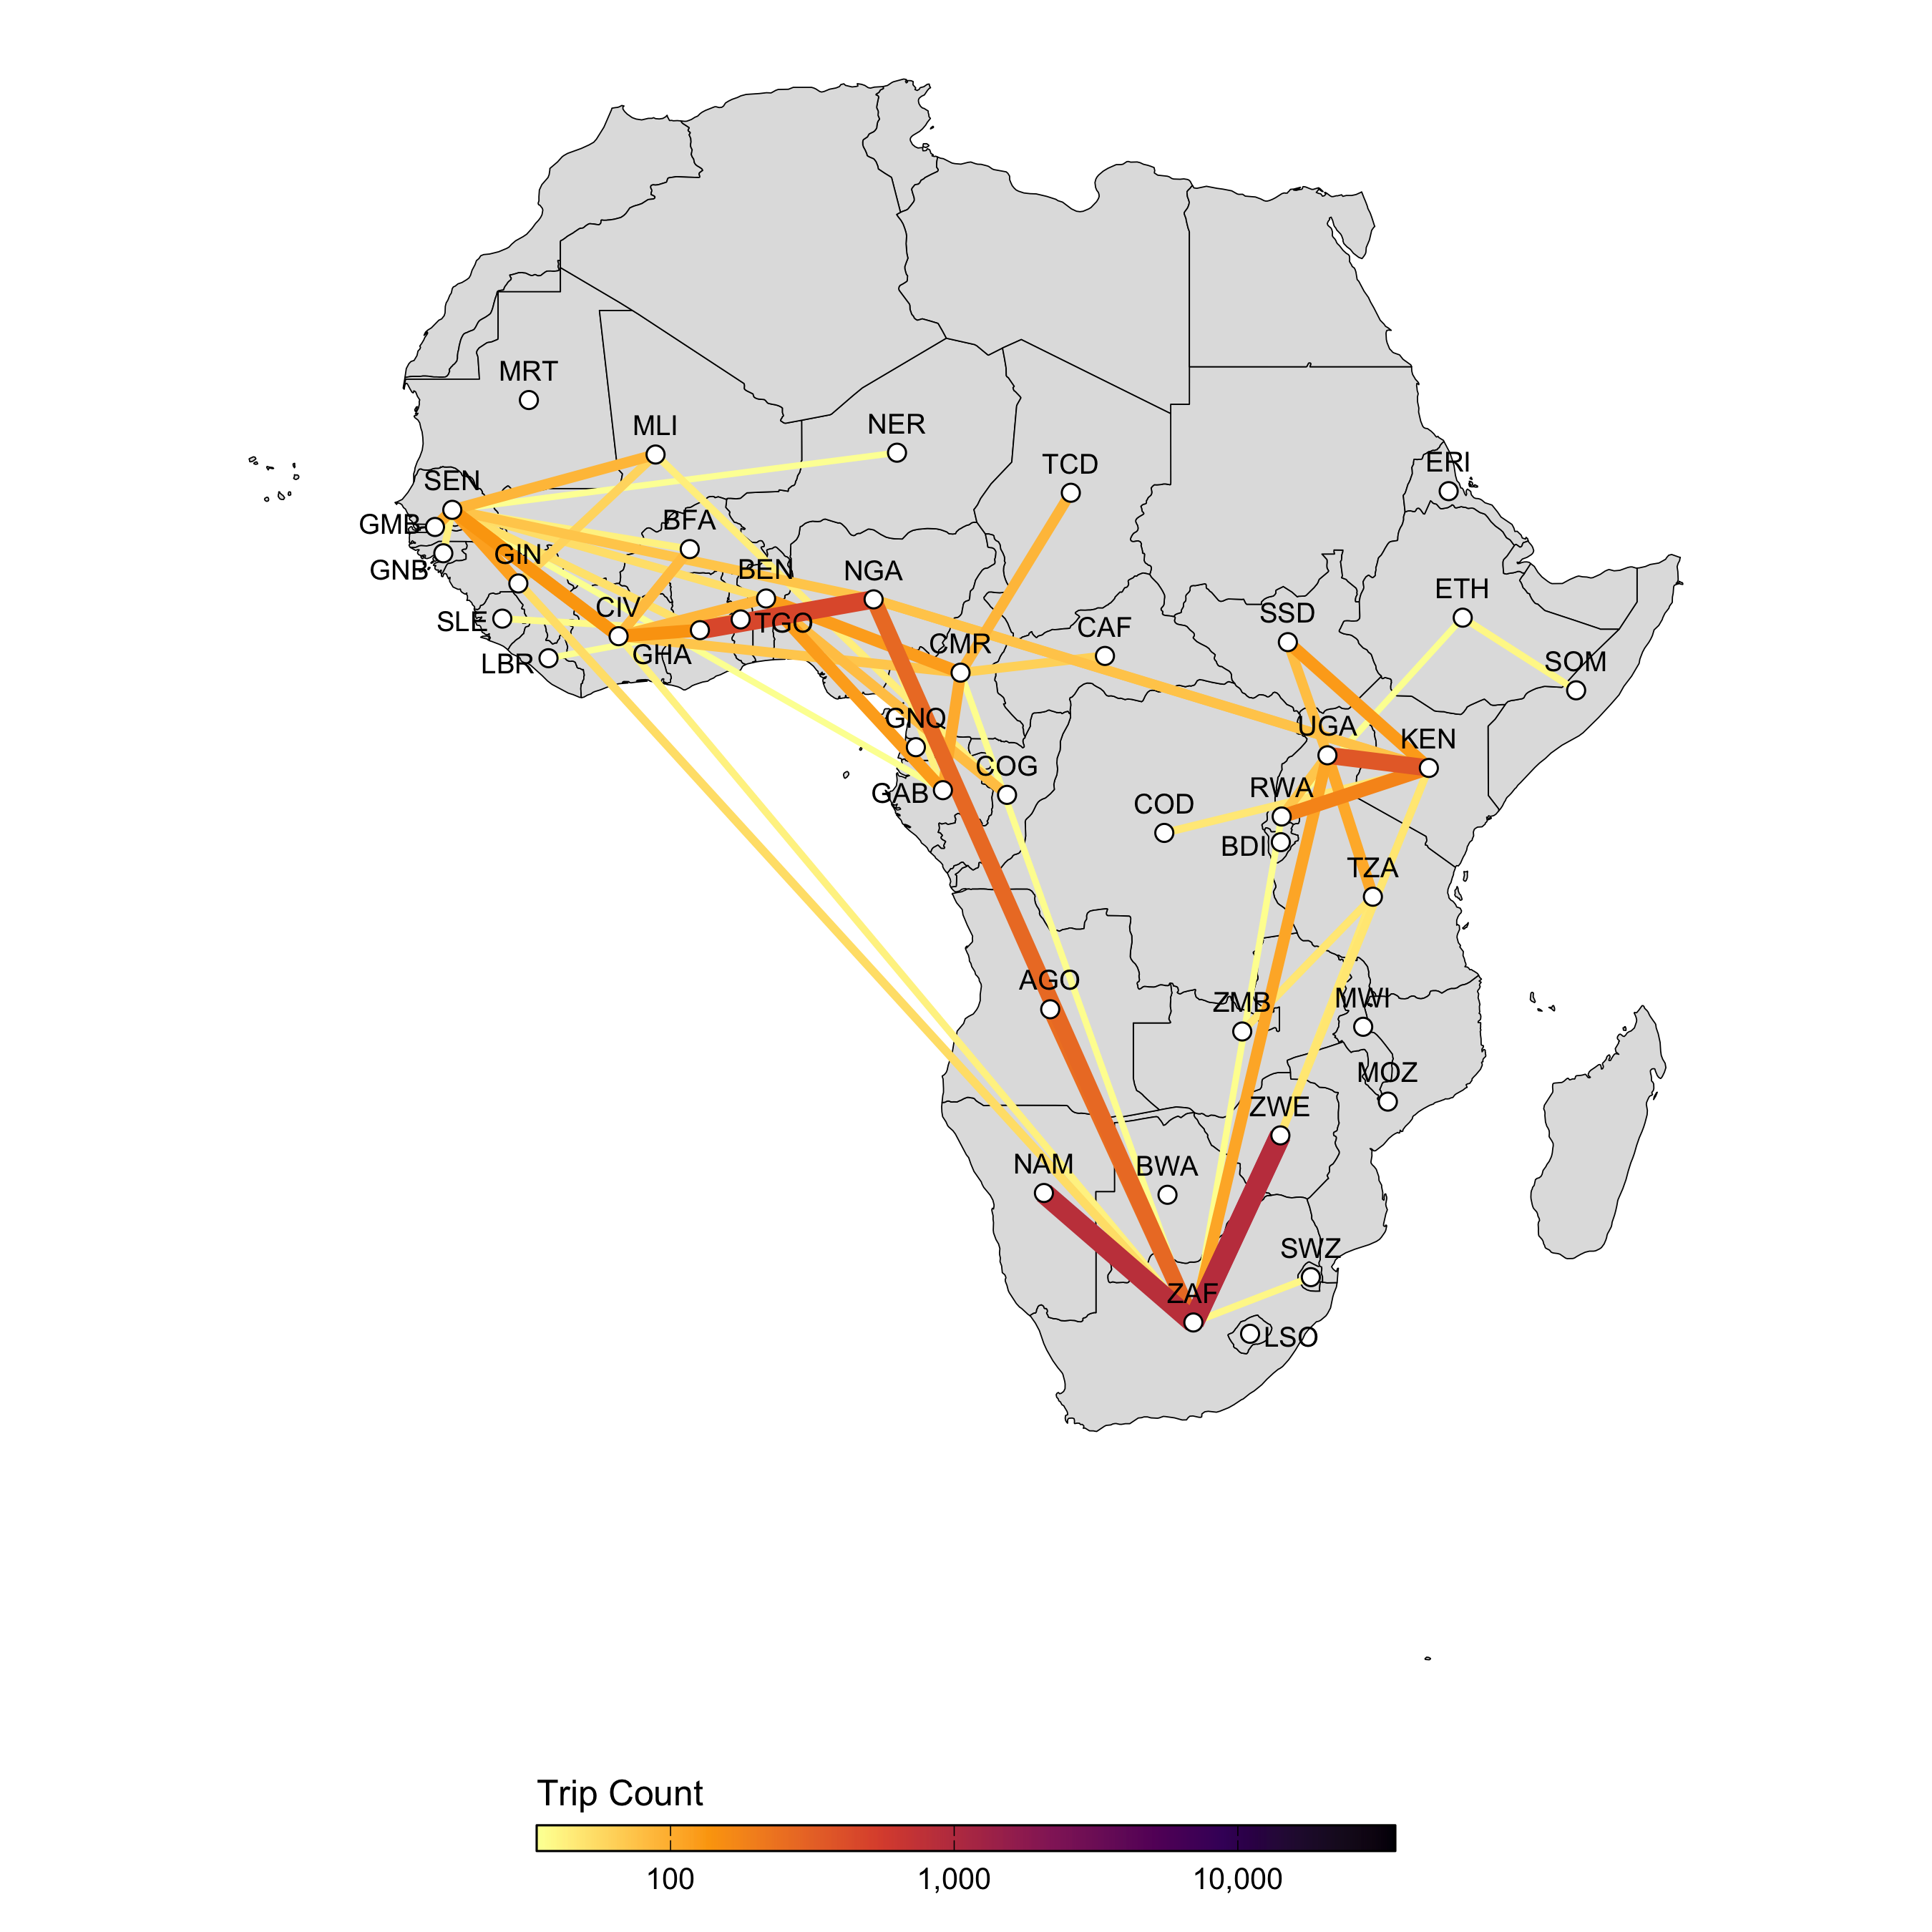
\includegraphics[width=1\linewidth]{figures/mobility_network} 

}

\caption{A network map showing the average number of air passengers per week in 2017.}\label{fig:mobility-network}
\end{figure}

\subsection{Human mobility model}\label{human-mobility-model}

The departure-diffusion model estimates diagonal and off-diagonal elements in the mobility matrix (\(M\)) separately and combines them using conditional probability rules. The model first estimates the probability of travel outside the origin location \(i\)---the departure process---and then the distribution of travel from the origin location \(i\) by normalizing connectivity values across all \(j\) destinations---the diffusion process. The values of \(\pi_{ij}\) sum to unity along each row, but the diagonal is not included, indicating that this is a relative quantity. That is to say, \(\pi_{ij}\) gives the probability of going from \(i\) to \(j\) given that travel outside origin \(i\) occurs. Therefore, we can use basic conditional probability rules to define the travel routes in the diagonal elements (trips made within the origin \(i\)) as
\[
\Pr( \neg \text{depart}_i ) =  1 - \tau_i
\]
and the off-diagonal elements (trips made outside origin \(i\)) as
\[
\Pr( \text{depart}_i, \text{diffuse}_{i \rightarrow j}) = \Pr( \text{diffuse}_{i \rightarrow j} \mid \text{depart}_i ) \Pr(\text{depart}_i ) = \pi_{ij} \tau_i.
\]
The expected mean number of trips for route \(i \rightarrow j\) is then:

\begin{equation}
M_{ij} = 
\begin{cases}
\theta N_i (1-\tau_i) \ & \text{if} \ i = j \\
\theta N_i \tau_i \pi_{ij} \ & \text{if} \ i \ne j.
\end{cases}
\label{eq:M}
\end{equation}

Where, \(\theta\) is a proportionality constant representing the overall number of trips per person in an origin population of size \(N_i\), \(\tau_i\) is the probability of leaving origin \(i\), and \(\pi_{ij}\) is the probability of travel to destination \(j\) given that travel outside origin \(i\) occurs.

\subsection{Estimating the departure process}\label{estimating-the-departure-process}

The probability of travel outside the origin is estimated for each location \(i\) to give the location-specific departure probability \(\tau_i\).
\[
\tau_i \sim \text{Beta}(1+s, 1+r)
\]
Binomial probabilities for each origin \(\tau_i\) are drawn from a Beta distributed prior with shape (\(s\)) and rate (\(r\)) parameters.
\[
\begin{aligned}
s &\sim \text{Gamma}(0.01, 0.01)\\
r &\sim \text{Gamma}(0.01, 0.01)
\end{aligned}
\]

\subsection{Estimating the diffusion process}\label{estimating-the-diffusion-process}

We use a normalized formulation of the power law gravity model to defined the diffusion process, the probability of travelling to destination \(j\) given travel outside origin \(i\) (\(\pi_{ij}\)) which is defined as:

\begin{equation}
\pi_{ij} = \frac{
N_j^\omega d_{ij}^{-\gamma}
}{
\sum\limits_{\forall j \ne i} N_j^\omega d_{ij}^{-\gamma}
}
\label{eq:gravity}
\end{equation}

Where, \(\omega\) scales the attractive force of each \(j\) destination based on its population size \(N_j\). The kernel function \(d_{ij}^{-\gamma}\) serves as a penalty on the proportion of travel from \(i\) to \(j\) based on distance. Prior distributions of diffusion model parameters are defined as:
\[
\begin{aligned}
\omega &\sim \text{Gamma}(1, 1)\\
\gamma &\sim \text{Gamma}(1, 1)
\end{aligned} 
\]

The models for \(\tau_i\) and \(\pi_{ij}\) were fitted to air traffic data from \href{https://www.oag.com/flight-data-sets}{OAG} using the \texttt{mobility} R package (\href{https://covid-19-mobility-data-network.github.io/mobility/}{Giles 2020}). Estimates for mobility model parameters are shown in Figures \ref{fig:mobility-departure} and \ref{fig:mobility-diffusion}.

\begin{figure}

{\centering 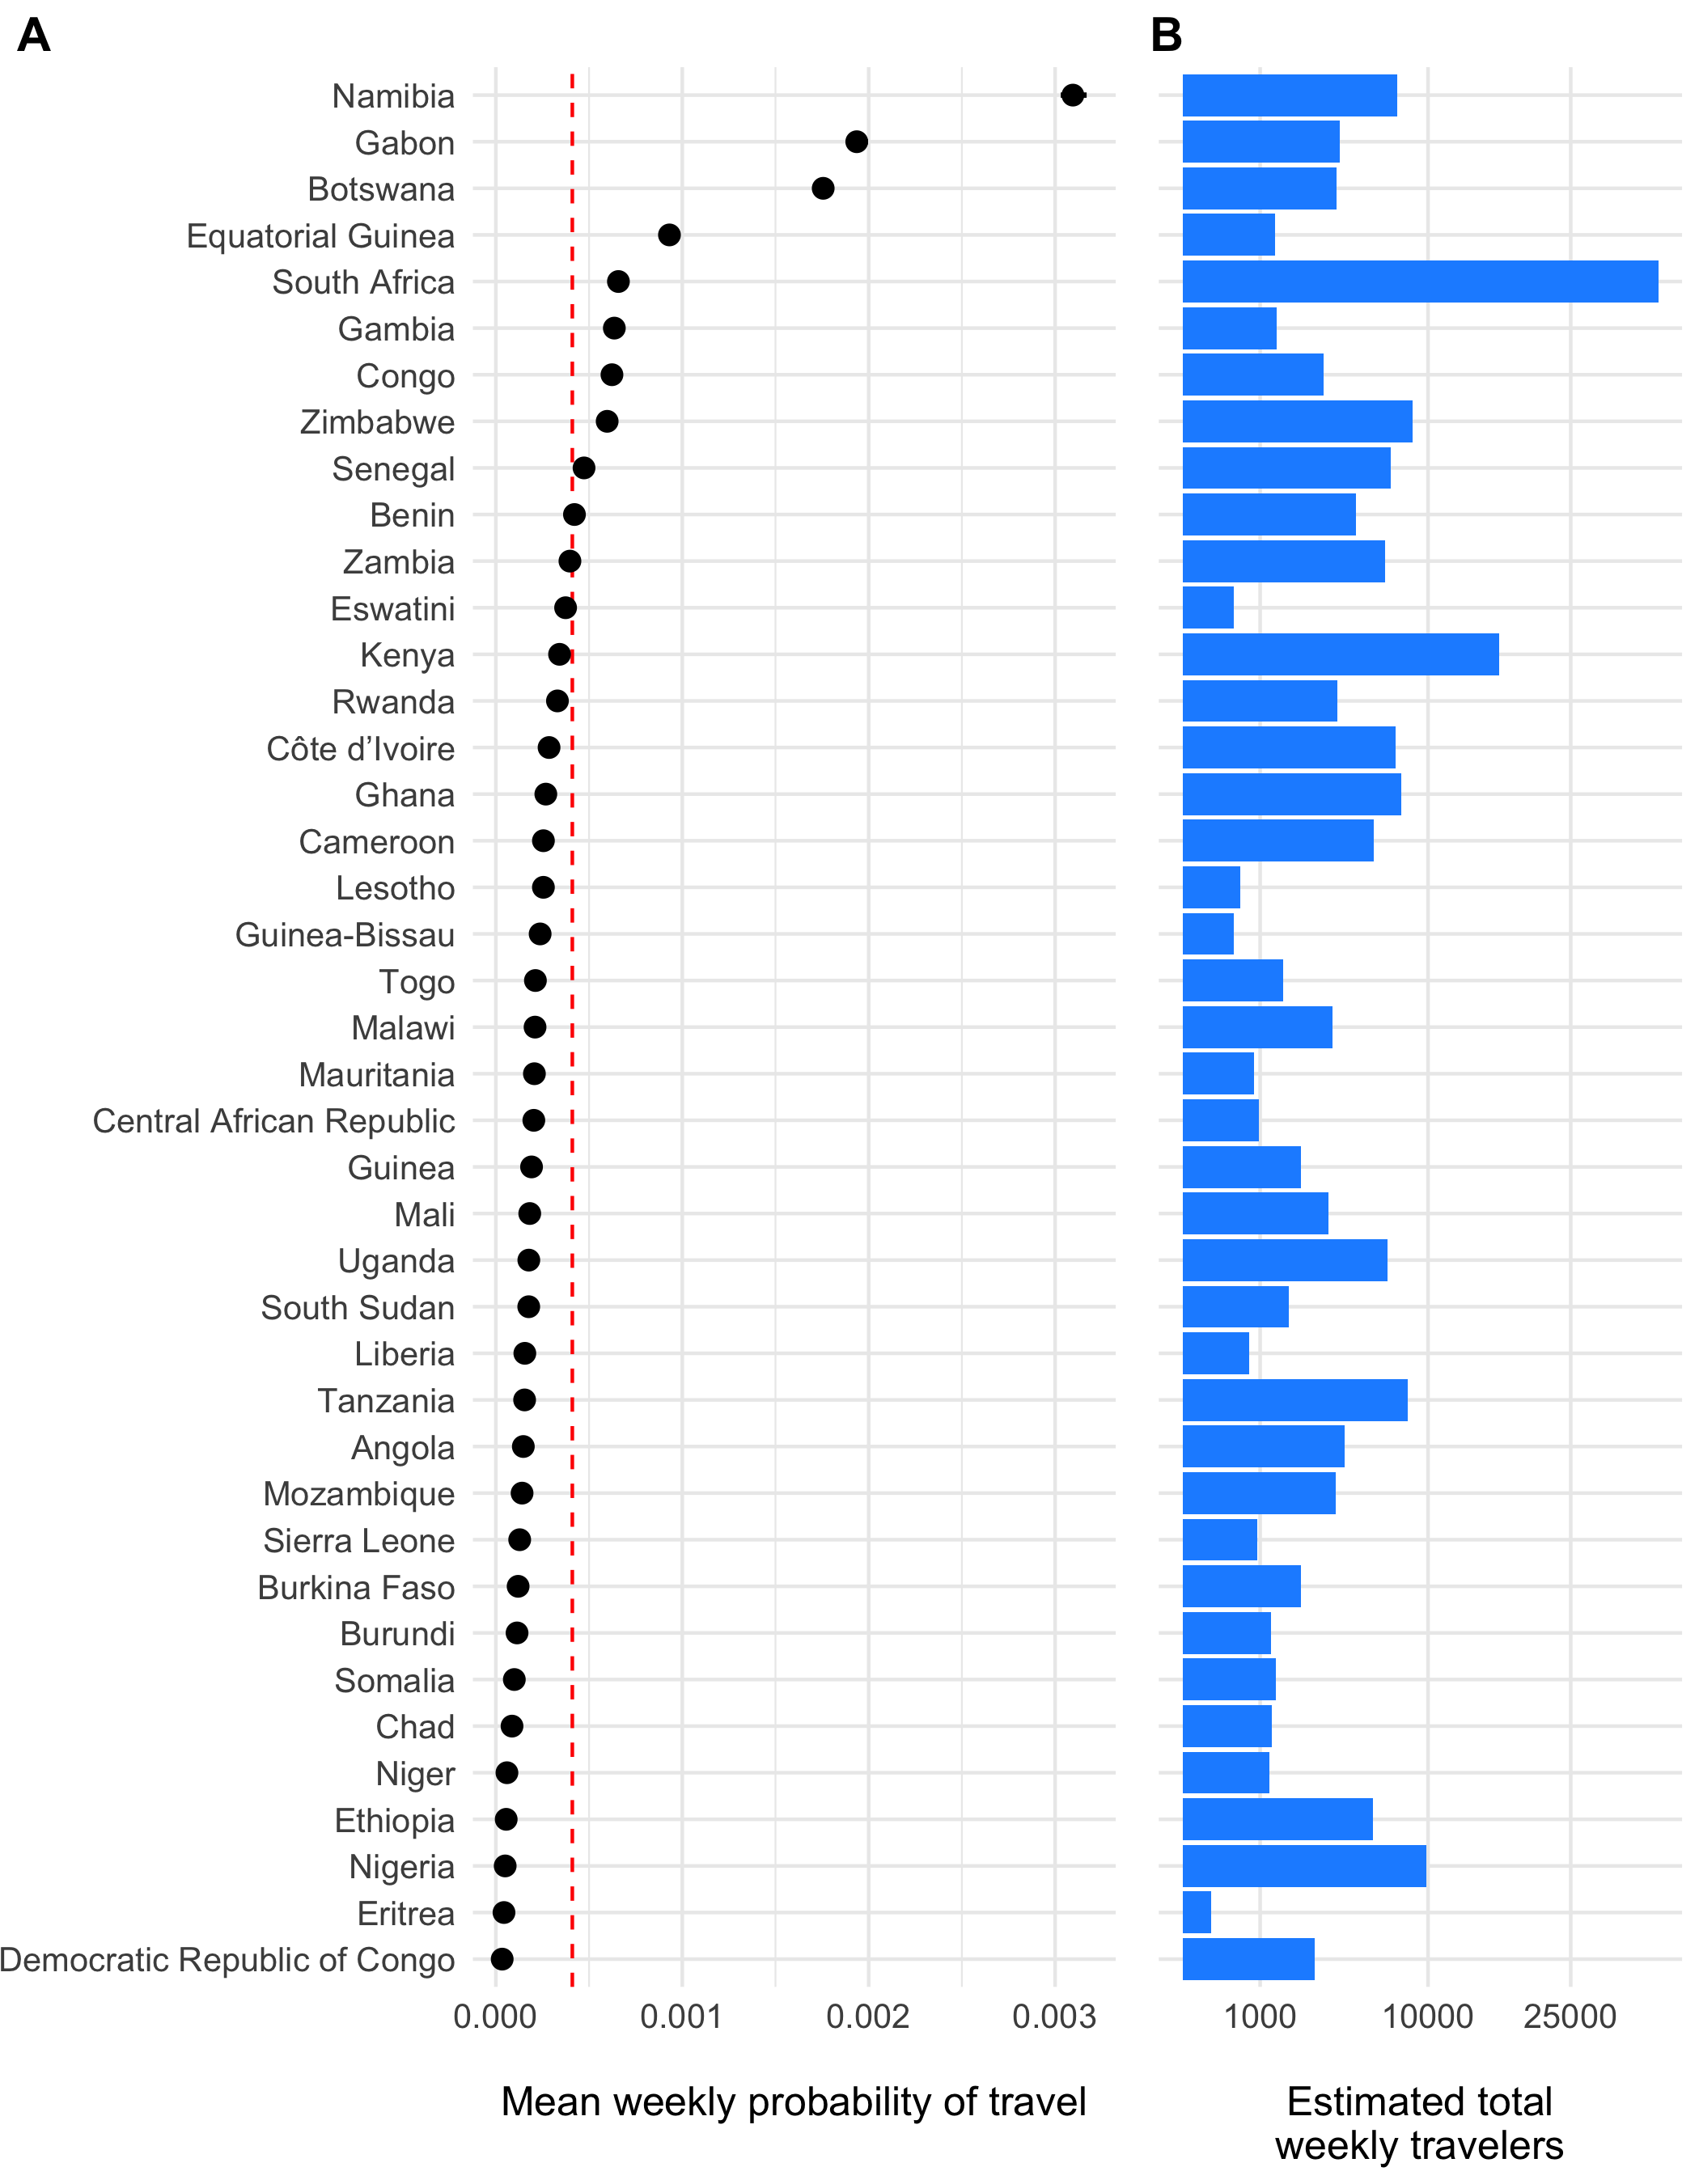
\includegraphics[width=1\linewidth]{figures/mobility_travel_prob_tau} 

}

\caption{The estimated weekly probability of travel outside of each origin location $\tau_i$ and 95\% confidence intervals is shown in panel A with the population mean indicated as a red dashed line. Panel B shows the estimated total number of travelers leaving origin $i$ each week.}\label{fig:mobility-departure}
\end{figure}

\begin{figure}

{\centering 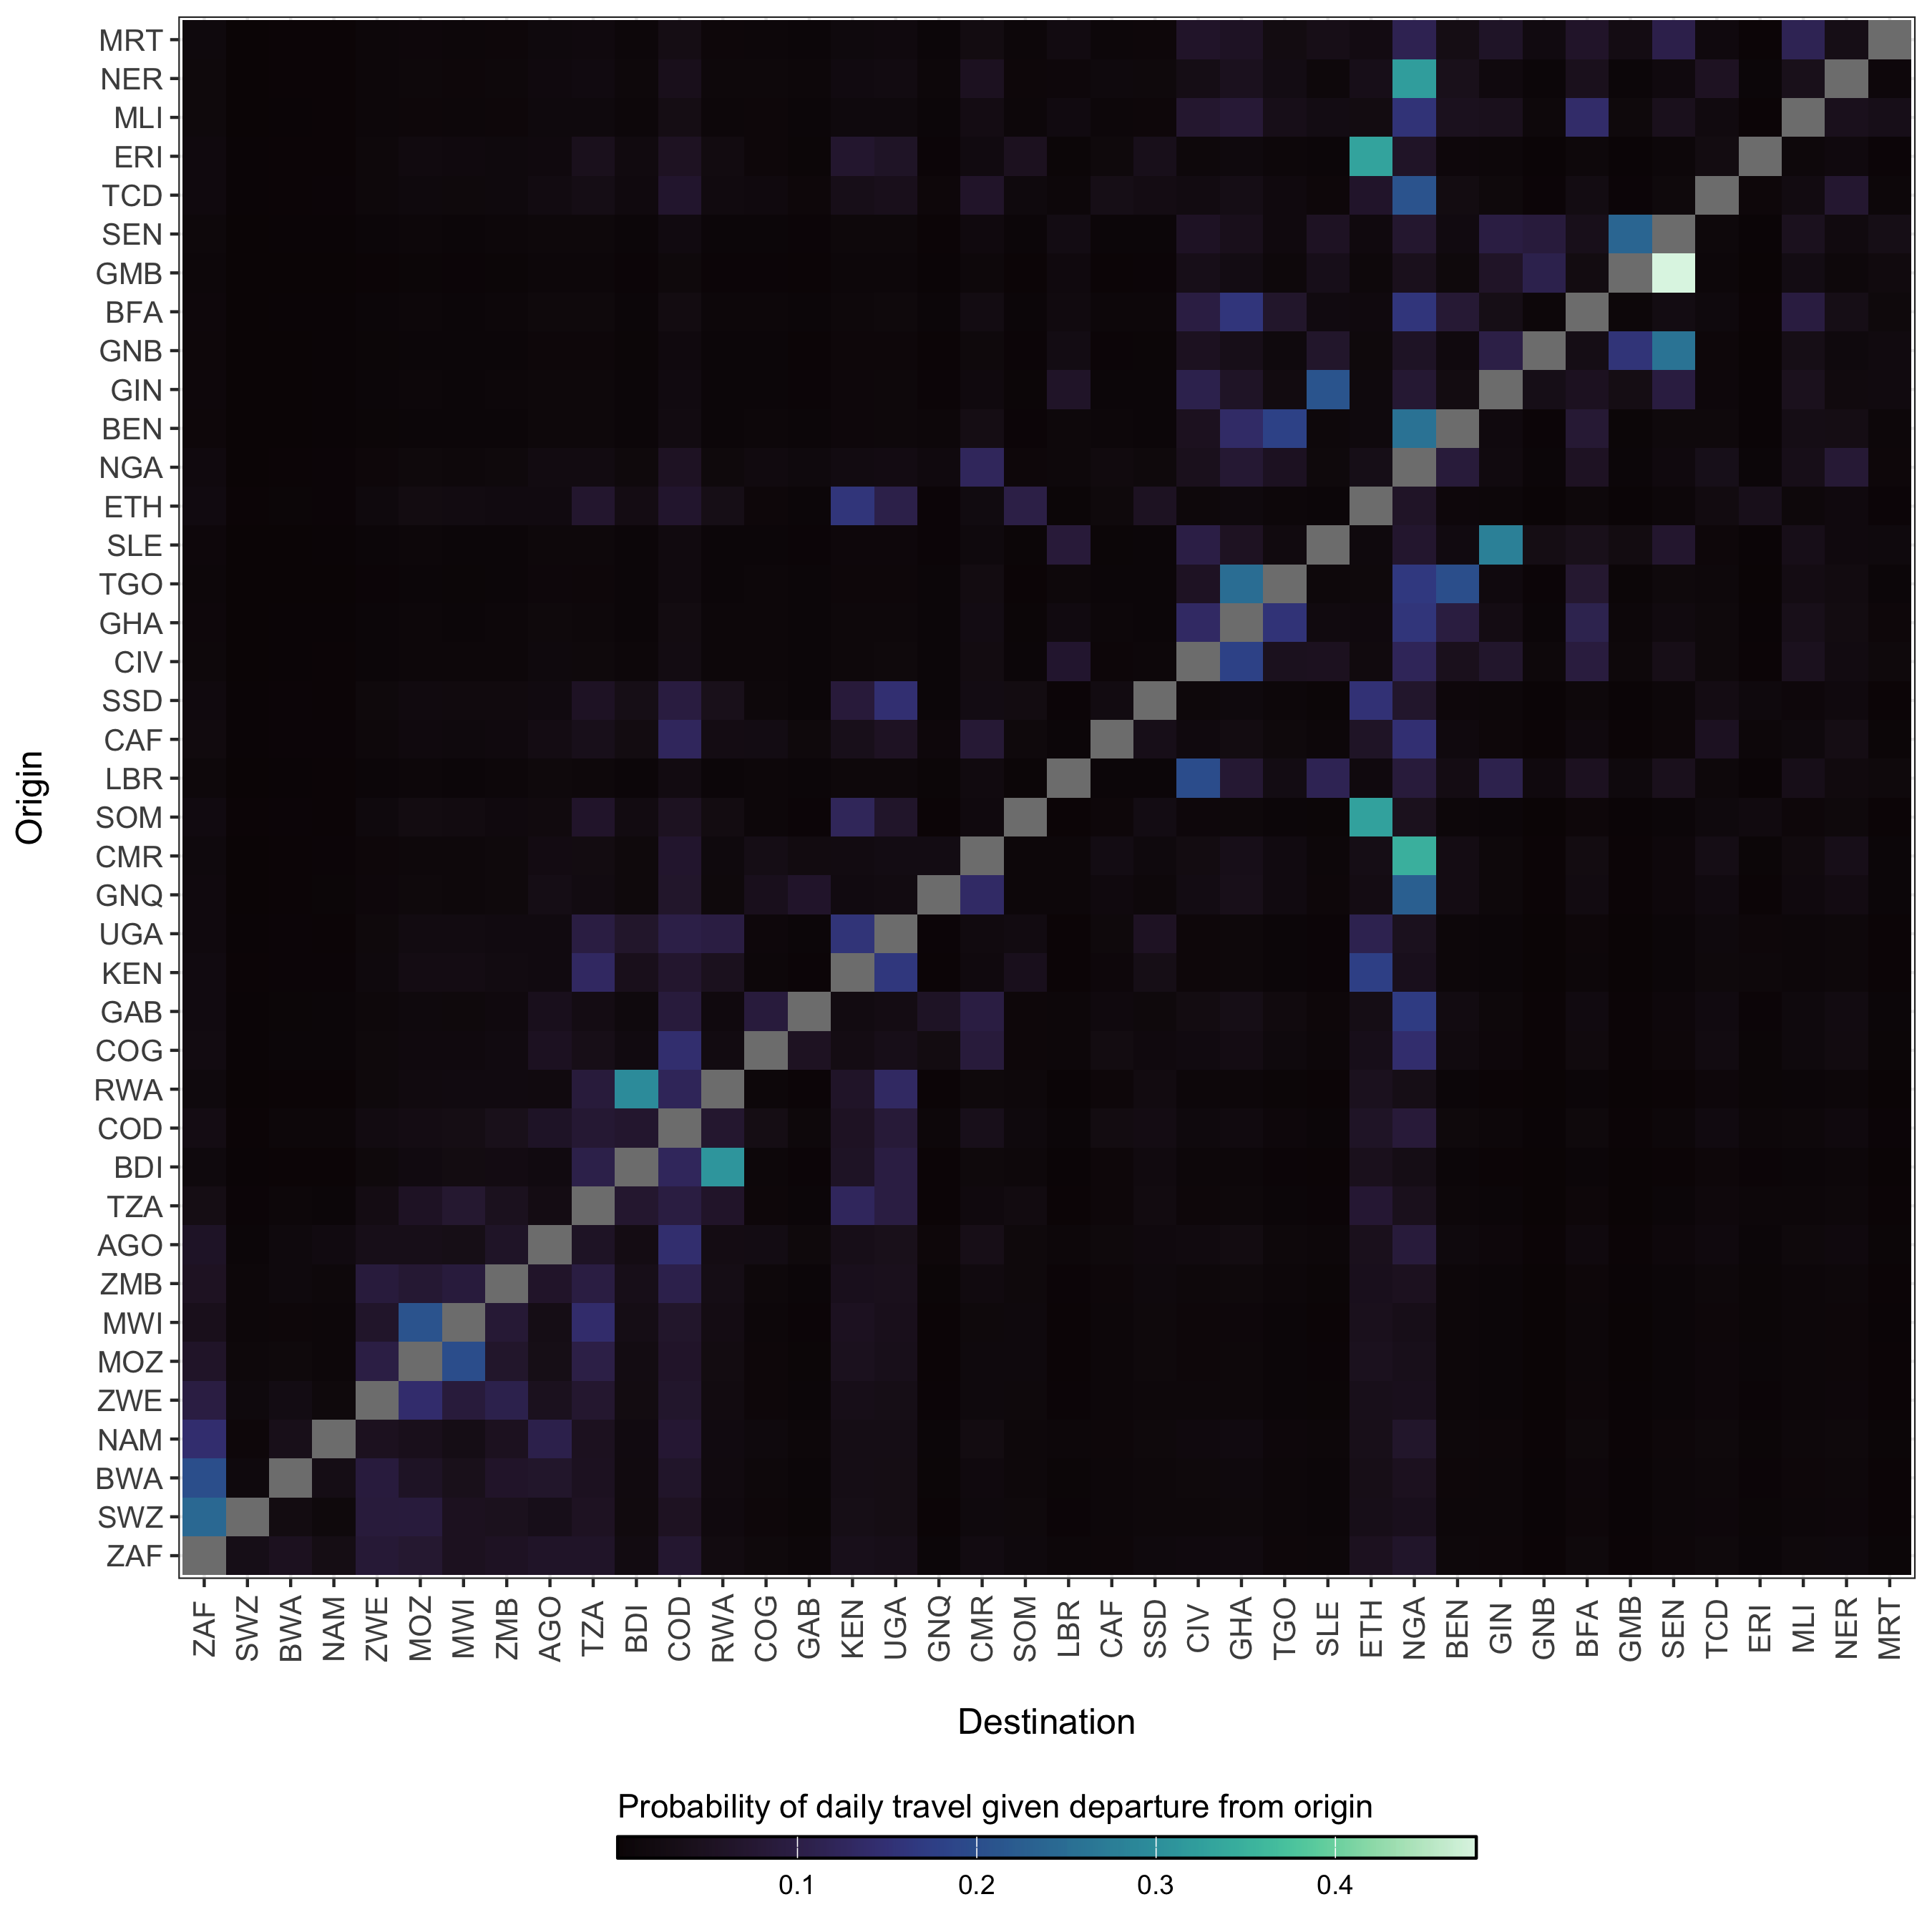
\includegraphics[width=1\linewidth]{figures/mobility_diffusion_pi} 

}

\caption{The diffusion process $\pi_{ij}$ which gives the estimated probability of travel from origin $i$ to destination $j$ given that travel outside of origin $i$ has occurred.}\label{fig:mobility-diffusion}
\end{figure}

\subsection{The probability of spatial transmission}\label{the-probability-of-spatial-transmission}

The likelihood of introductions of cholera from disparate locations is a major concern during cholera outbreaks. However, this can be difficult to characterize given the endemic dynamics and patterns of human movement. We include a few measures of spatial heterogeneity here and the first is a simple importation probability based on connectivity and the possibility of incoming infections. The basic probability of transmission from an origin \(i\) to a particular destination \(j\) and time \(t\) is defined as:

\begin{equation} 
p(i,j,t) = 1 - e^{-\beta_{jt}^{\text{hum}} (((1-\tau_j)S_{jt})/N_{jt}) \pi_{ij}\tau_iI_{it}}
\label{eq:prob}
\end{equation}

\subsection{The spatial hazard}\label{the-spatial-hazard}

Although we are more concerned with endemic dynamics here, there are likely to be periods of time early in the rainy season where cholera cases and the rate of transmission is low enough for spatial spread to resemble epidemic dynamics for a time. During such times periods, we can estimate the arrival time of contagion for any location where cases are yet to be reported. We do this be estimating the spatial hazard of transmission:

\begin{equation} 
h(j,t) = \frac{
\beta_{jt}^{\text{hum}} \Big(1 - \exp\big(-((1-\tau_j)S_{jt}/N_{jt}) \sum_{\forall i \not= j} \pi_{ij}\tau_i (I_{it}/N_{it}) \big) \Big)
}{
1/\big(1 + \beta_{jt}^{\text{hum}} (1-\tau_j)S_{jt}\big)
}.
\label{eq:hazard}
\end{equation}

And then normalizing to give the waiting time distribution for all locations:

\begin{equation} 
w(j,t) = h(j,T) \prod_{t=1}^{T-1}1-h(j,t).
\label{eq:waiting}
\end{equation}

\subsection{Coupling among locations}\label{coupling-among-locations}

Another measure of spatial heterogeneity is to quantify the coupling of disease dynamics among metapopulations using a correlation coefficient. Here, we use the definition of spatial correlation between locations \(i\) and \(j\) as \(C_{ij}\) described in \href{https://onlinelibrary.wiley.com/doi/abs/10.1046/j.1461-0248.2002.00268.x}{Keeling and Rohani (2002)}, which gives a measure of how similar infection dynamics are between locations.

\begin{equation} 
C_{ij} = \frac{
( y_{it} - \bar{y}_i )( y_{jt} - \bar{y}_j )
}{
\sqrt{\text{var}(y_i) \text{var}(y_j)}
}
\label{eq:correlation}
\end{equation}
Where \(y_{it} = I_{it}/N_i\) and \(y_{jt} = I_{jt}/N_j\). Mean prevalence in each location is \(\bar{y_i} = \frac{1}{T} \sum_{t=1}^{T} y_{it}\) and \(\bar{y_j} = \frac{1}{T} \sum_{t=1}^{T} y_{jt}\).

\section{The observation process}\label{the-observation-process}

\subsection{Rate of symptomatic infection}\label{rate-of-symptomatic-infection}

The presentation of infection with \emph{V. cholerae} can be extremely variable. The severity of infection depends many factors such as the amount of the infectious dose, the age of the host, the level of immunity of the host either through vaccination or previous infection, and naivety to the particular strain of \emph{V. cholerae}. Additional circumstantial factors such as nutritional status and overall pathogen burden may also impact infection severity. At the population level, the observed proportion of infections that are symptomatic is also dependent on the endemicity of cholera in the region. Highly endemic areas (e.g.~parts of Bangladesh; \href{https://www.nature.com/articles/s41591-024-02810-4}{Hegde et al 2024}) may have a very low proportion of symptomatic infections due to many previous exposures. Inversely, populations that are largely naive to \emph{V. cholerae} will exhibit a relatively higher proportion of symptomatic infections (e.g.~Haiti; \href{https://www.ncbi.nlm.nih.gov/pmc/articles/PMC10635253/}{Finger et al 2024}).

Accounting for all of these nuances in the first version of this model not possible, but we can past studies do contain some information that can help to set some sensible bounds on our definition for the proportion of infections that are symptomatic (\(\sigma\)). So we have compiled a short list of studies that have done sero-surveys and cohort studies to assess the likelihood of symptomatic infections in different locations and displayed those results in Table (\ref{tab:symptomatic-table}).

To provide a reasonably informed prior for the proportion of infections that are symptomatic, we calculated the combine mean and confidence intervals of all studies in Table \ref{tab:symptomatic-table} and fit a Beta distribution that corresponds to these quantiles using least-squares and a Nelder-Mead algorithm. The resulting prior distribution for the symptomatic proportion \(\sigma\) is:

\begin{equation}
\sigma \sim \text{Beta}(4.30, 13.51)
\end{equation}

\begin{table}

\caption{\label{tab:symptomatic-table}Summary of Studies on Cholera Immunity}
\centering
\begin{tabular}[t]{r|r|r|l|l|l}
\hline
Mean & Low CI & High CI & Location & Source & Note\\
\hline
0.570 & NA & NA & NA & [Nelson et al (2009)](https://www.ncbi.nlm.nih.gov/pmc/articles/PMC3842031/) & Review\\
\hline
NA & 1.000 & 0.250 & NA & [Lueng \& Matrajt (2021)](https://journals.plos.org/plosntds/article?id=10.1371/journal.pntd.0009383) & Review\\
\hline
NA & 0.600 & 0.200 & Endemic regions & [Harris et al (2012)](https://www.sciencedirect.com/science/article/pii/S014067361260436X) & Review\\
\hline
0.238 & 0.250 & 0.227 & Haiti & [Finger et al (2024)](https://www.ncbi.nlm.nih.gov/pmc/articles/PMC10635253/) & Sero-survey and clinical data\\
\hline
0.213 & 0.231 & 0.194 & Haiti & [Jackson et al (2013)](https://www.ajtmh.org/view/journals/tpmd/89/4/article-p654.xml) & Cross-sectional sero-survey\\
\hline
0.204 & NA & NA & Pakistan & [Bart et al (1970)](https://doi.org/10.1093/infdis/121.Supplement.S17) & Sero-survey during epidemic; El Tor Ogawa strain\\
\hline
0.371 & NA & NA & Pakistan & [Bart et al (1970)](https://doi.org/10.1093/infdis/121.Supplement.S17) & Sero-survey during epidemic; Inaba strain\\
\hline
0.184 & 0.256 & 0.112 & Bangladesh & [Harris et al (2008)](https://journals.plos.org/plosntds/article?id=10.1371/journal.pntd.0000221) & Household cohort; mean of all age groups\\
\hline
0.001 & 0.000 & 0.001 & Bangladesh & [Hegde et al (2024)](https://www.nature.com/articles/s41591-024-02810-4) & Sero-survey and clinical data\\
\hline
\end{tabular}
\end{table}

The prior distribution for \(\sigma\) is plotted in Figure \ref{fig:symptomatic-fig}A with the reported values of the proportion symptomatic from previous studies shown in \ref{fig:symptomatic-fig}B.

\begin{figure}

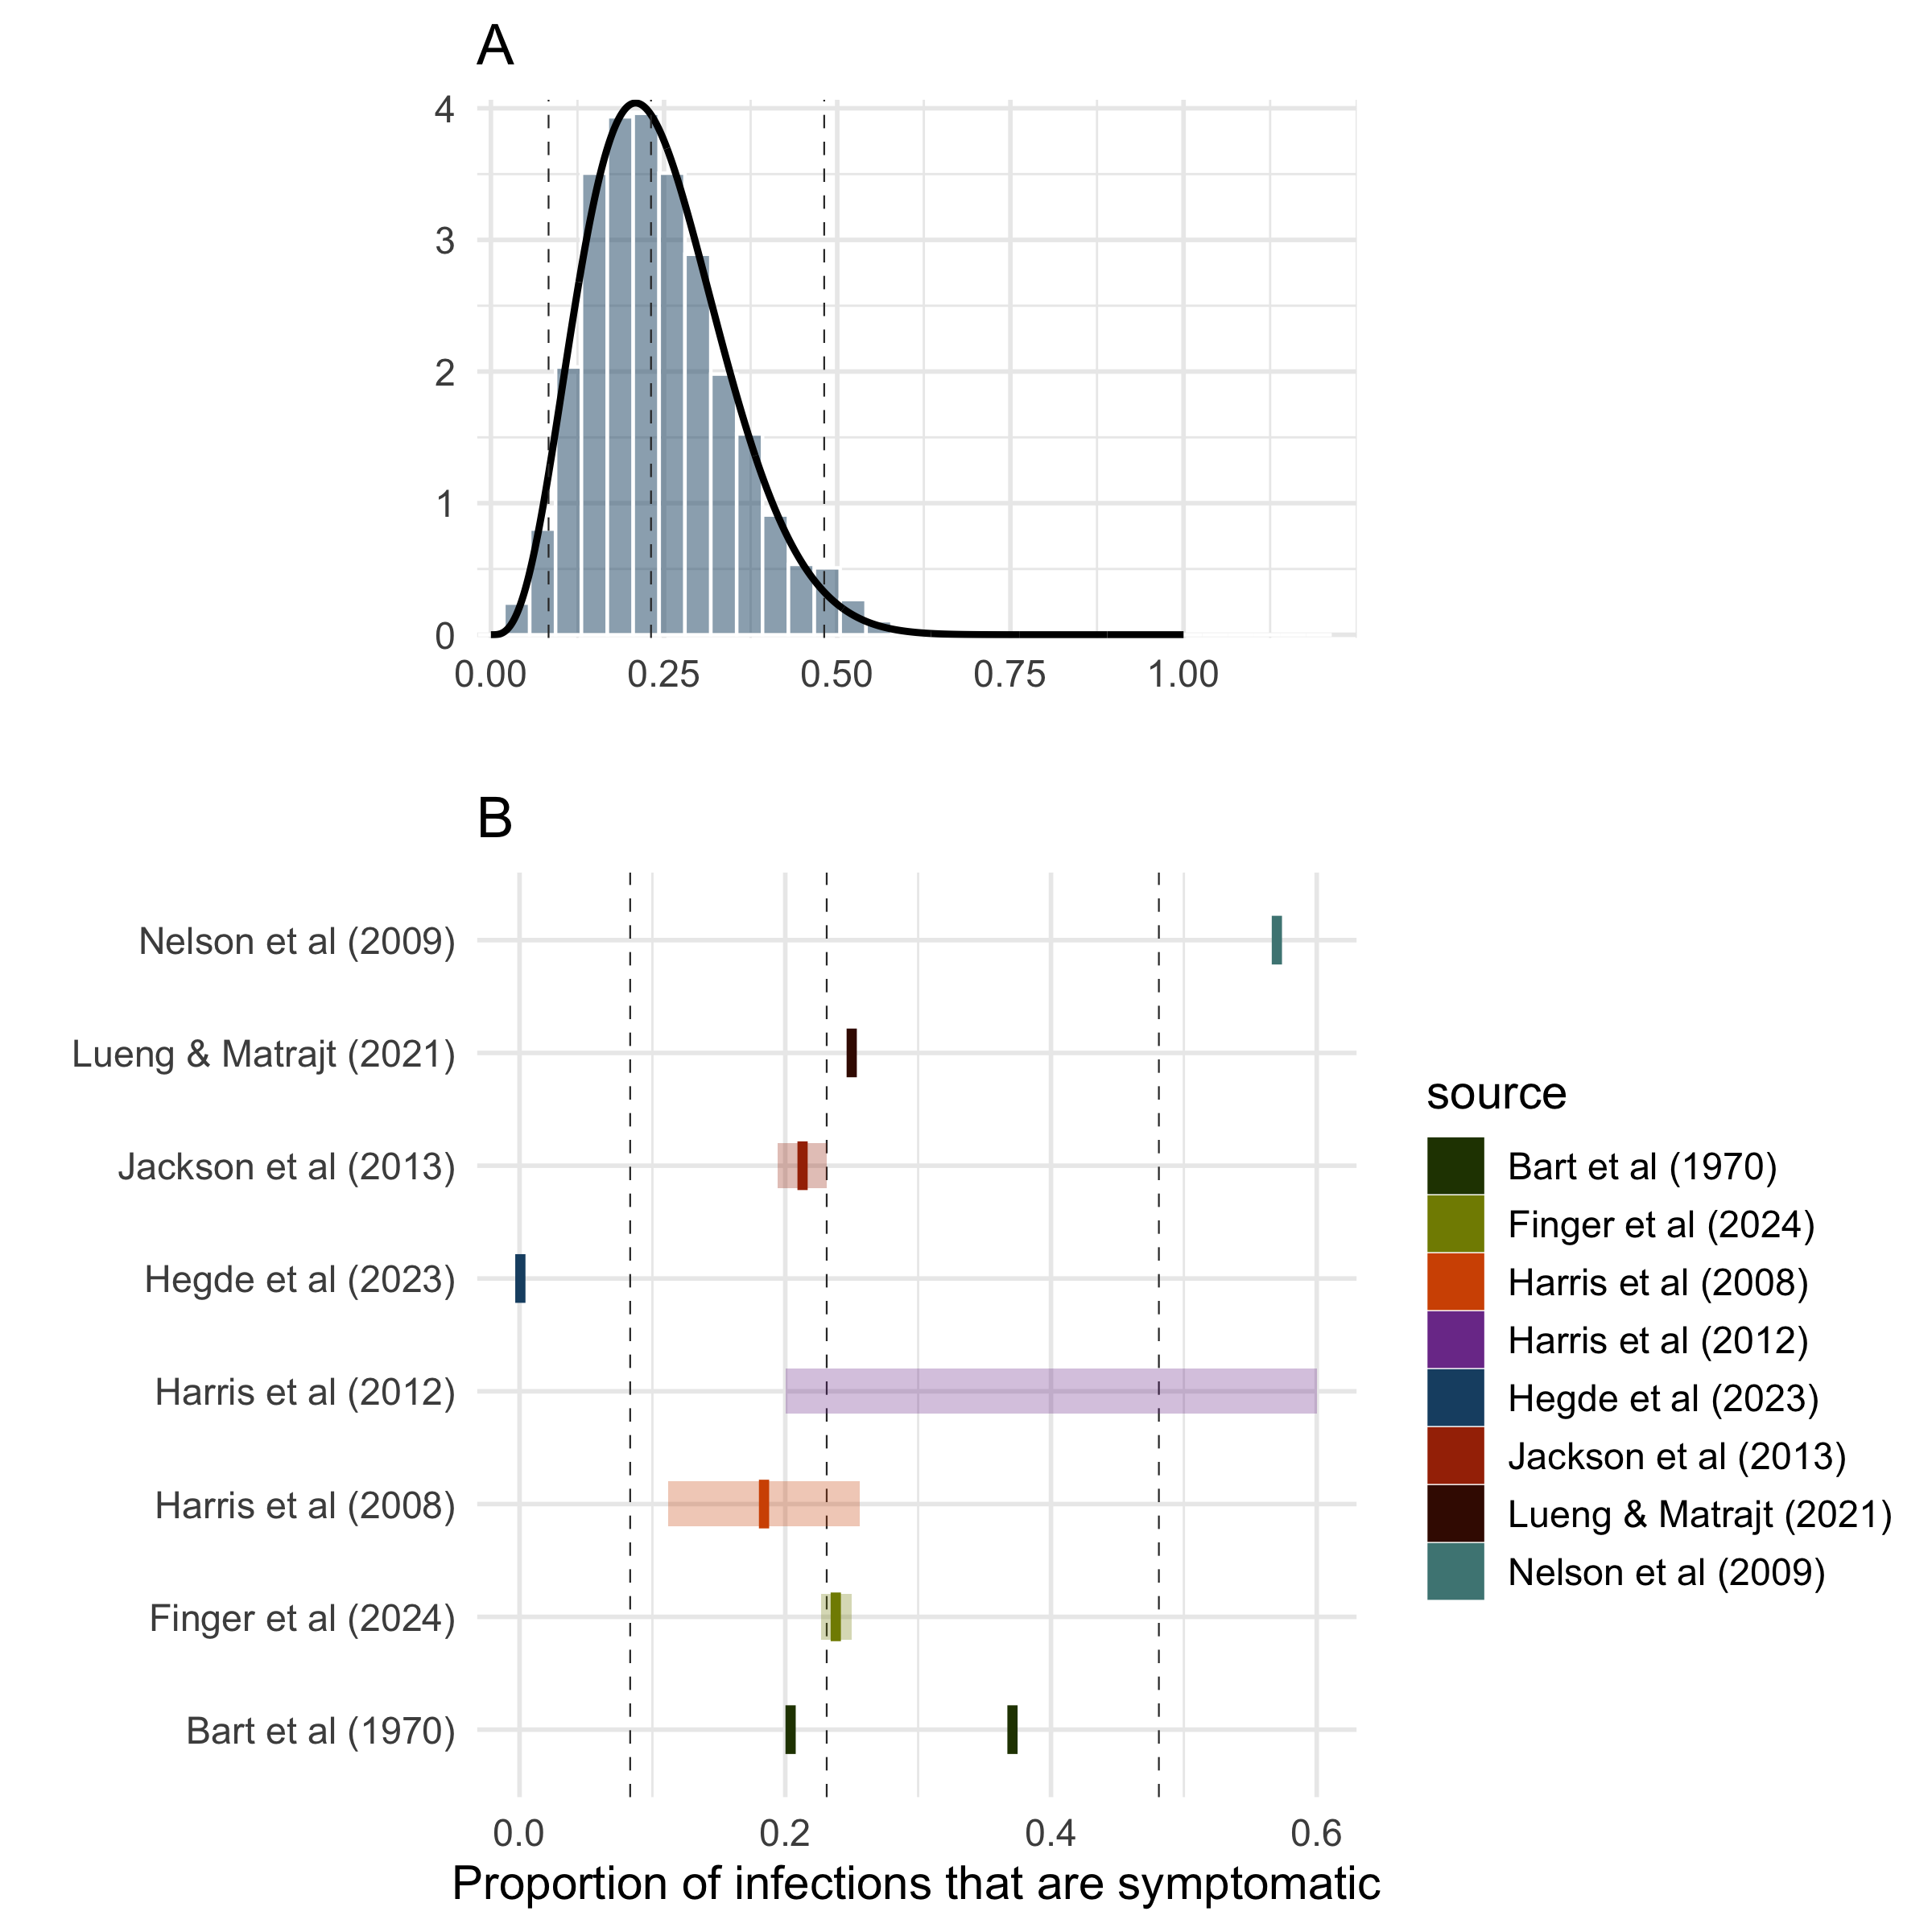
\includegraphics[width=1.03\linewidth]{figures/proportion_symptomatic} \hfill{}

\caption{Proportion of infections that are symptomatic.}\label{fig:symptomatic-fig}
\end{figure}

\subsection{Suspected cases}\label{suspected-cases}

The clinical presentation of diarrheal diseases is often similar across various pathogens, which can lead to systematic biases in the reported number of cholera cases. It is anticipated that the number of suspected cholera cases is related to the actual number of infections by a factor of \(1/\rho\), where \(\rho\) represents the proportion of suspected cases that are true infections. To adjust for this bias, we use estimates from the meta-analysis by \href{https://journals.plos.org/plosmedicine/article?id=10.1371/journal.pmed.1004286}{Weins et al.~(2023)}, which suggests that suspected cholera cases outnumber true infections by approximately 2 to 1, with a mean across studies indicating that 52\% (24-80\% 95\% CI) of suspected cases are actual cholera infections. A higher estimate was reported for ourbreak settings (78\%, 40-99\% 95\% CI). To account for the variability in this estimate, we fit a Beta distribution to the reported quantiles using a least squares approach and the Nelder-Mead algorithm, resulting in the prior distribution shown in Figure \ref{fig:rho}B:

\begin{equation}
\rho \sim \text{Beta}(4.79, 1.53).
\end{equation}

\begin{figure}

{\centering 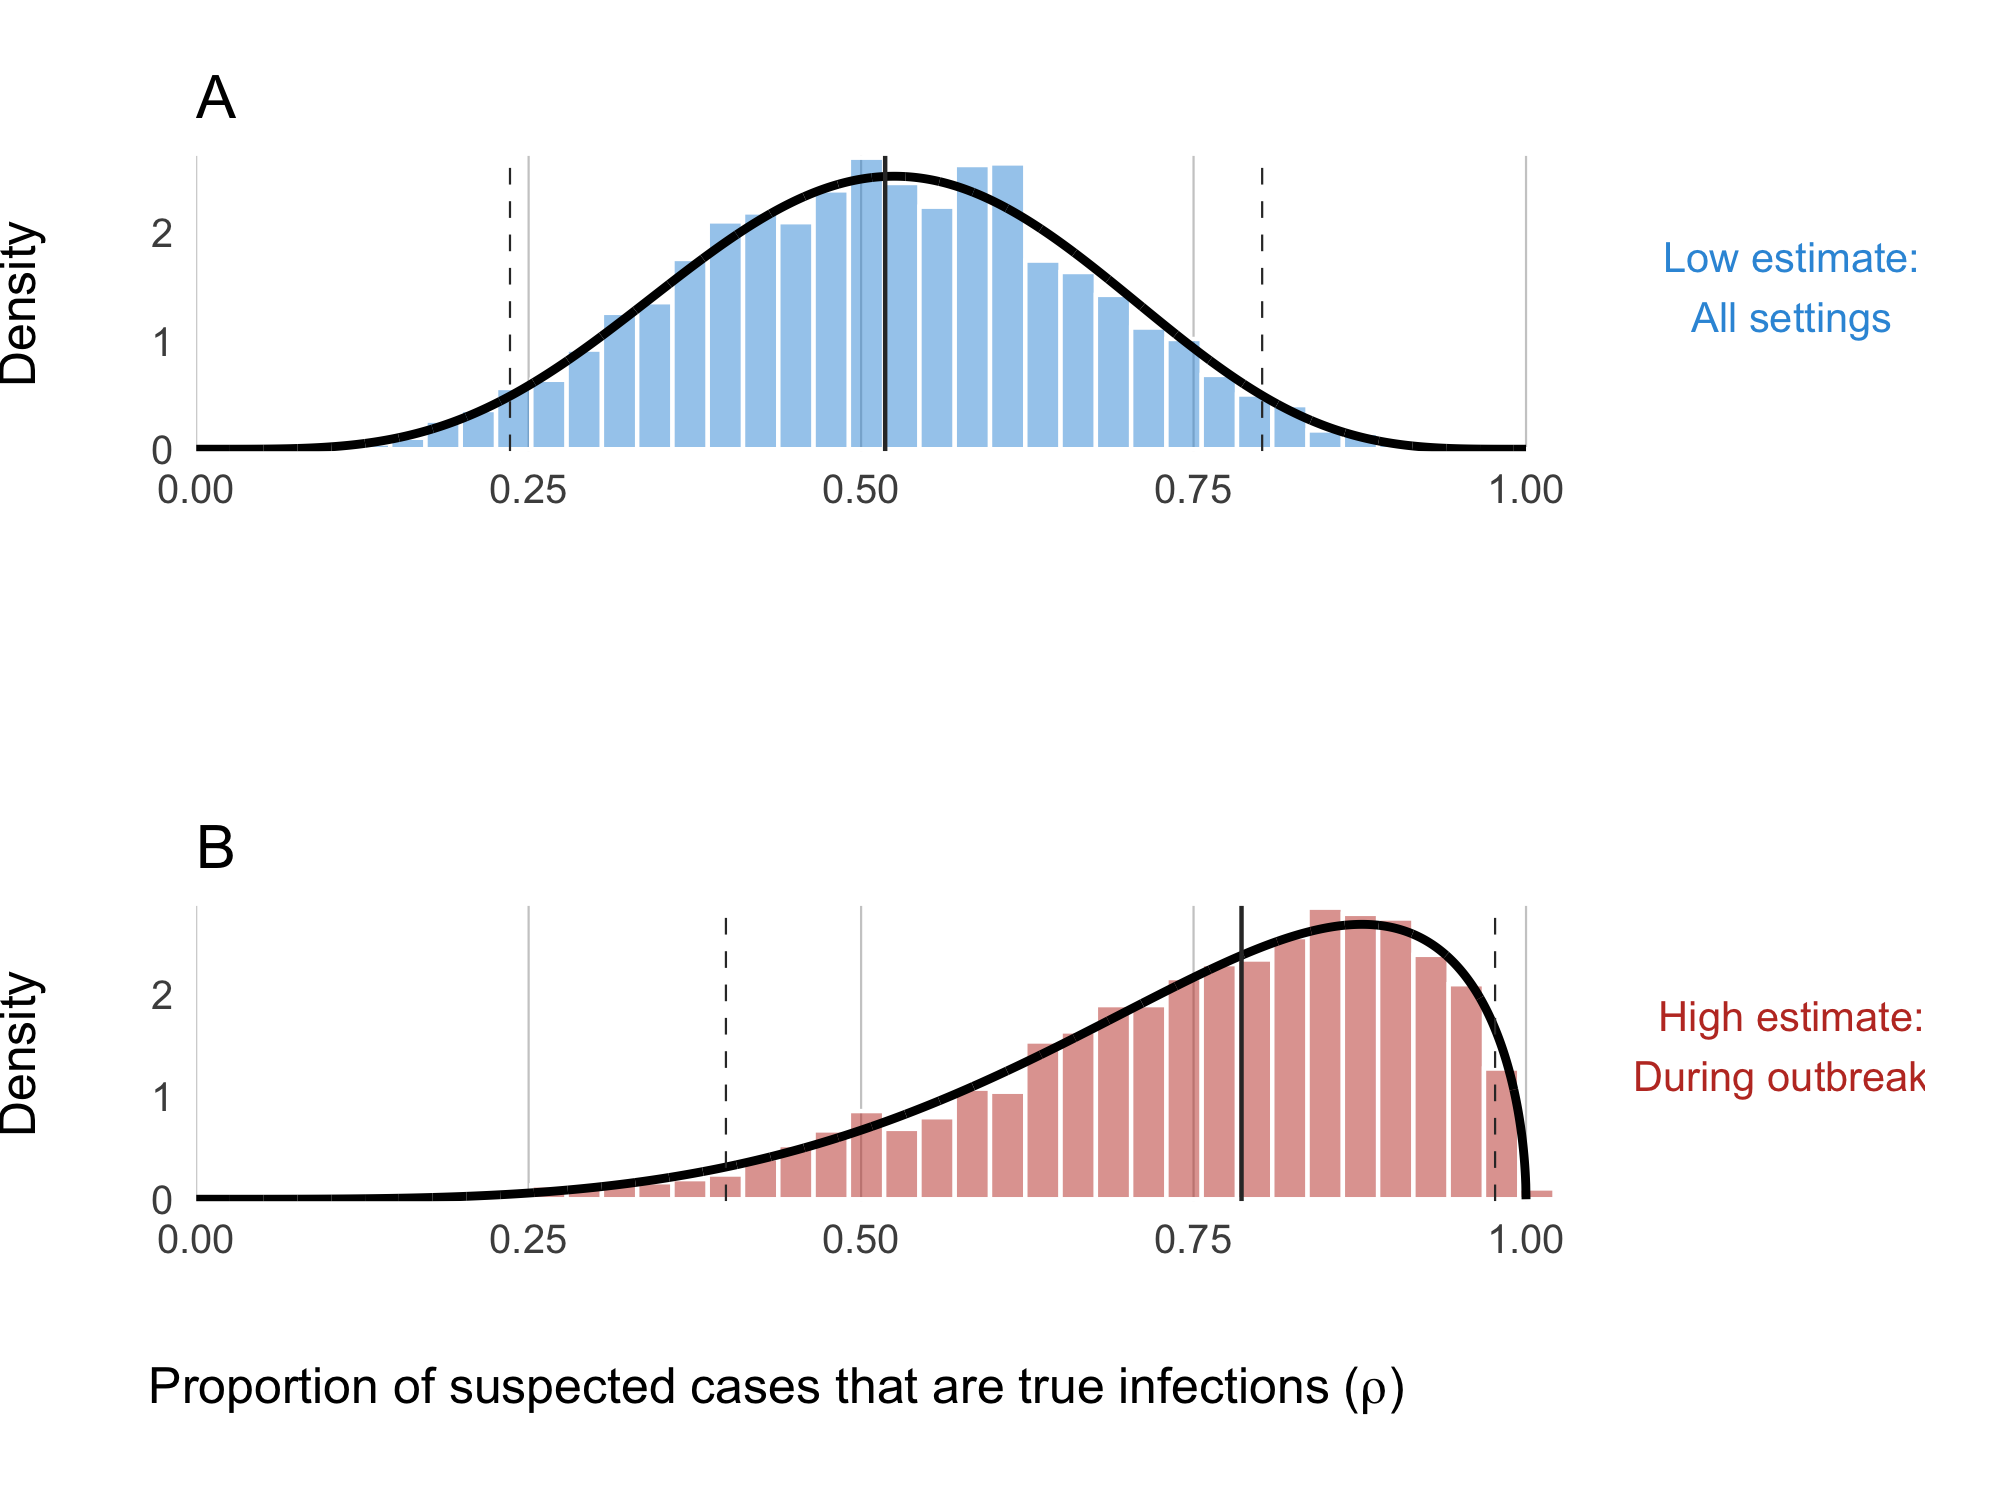
\includegraphics[width=1\linewidth]{figures/suspected_cases} 

}

\caption{Proportion of suspected cholera cases that are true infections. Panel A shows the 'low' assumption which estimates across all settings: $\rho \sim \text{Beta}(5.43, 5.01)$. Panel B shows the 'high' assumption where the estimate reflects high-quality studies during outbreaks: $\rho \sim \text{Beta}(4.79, 1.53)$}\label{fig:rho}
\end{figure}

\subsection{Case fatality rate}\label{case-fatality-rate}

The Case Fatality Rate (CFR) among symptomatic infections was calculated using reported cases and deaths data from January 2021 to August 2024. The data were collated from various issues of the WHO Weekly Epidemiological Record the Global Cholera and Acute Watery Diarrhea (AWD) Dashboard (see Data section) which provide annual aggregations of reported cholera cases and deaths. We then used the Binomial exact test (\href{https://www.rdocumentation.org/packages/stats/versions/3.6.2/topics/binom.test}{\texttt{binom.test}} in R) to calculate the mean probability for the number of deaths (successes) given the number of reported cases (sample size), and the \href{https://en.wikipedia.org/wiki/Binomial_proportion_confidence_interval\#Clopper\%E2\%80\%93Pearson_interval}{Clopper-Pearson method} for calculating the binomial confidence intervals. We then fit Beta distributions to the mean CFR and 95\% confidence intervals calculated for each country using least squares and the Nelder-Mead algorithm to give the distributional uncertainty around the CFR estimate for each country (\(\mu_j\)).

\[
\mu_j \sim \text{Beta}(s_{1,j}, s_{2,j})
\]

Where \(s_{1,i}\) and \(s_{2,j}\) are the two positive shape parameters of the Beta distribution estimated for destination \(j\). By definition \(\mu_j\) is the CFR for reported cases which are a subset of the total number of infections. Therefore, to infer the total number of deaths attributable to cholera infection, we assume that the CFR of observed cases is proportionally equivalent to the CFR of all cases and then calculate total deaths \(D\) as follows:

\begin{equation}
\begin{aligned}
\text{CFR}_{\text{observed}} &= \text{CFR}_{\text{total}}\\
\\[3pt]
\frac{[\text{observed deaths}]}{[\text{observed cases}]} &= 
\frac{[\text{total deaths}]}{[\text{all infections}]}\\
\\[3pt]
\text{total deaths} &= \frac{[\text{observed deaths}] \times [\text{true infections}]}{[\text{observed cases}]}\\
\\[3pt]
D_{jt} &= \frac{ [\sigma\rho\mu_j I_{jt}] \times [I_{jt}] }{ [\sigma\rho I_{jt}] }
\end{aligned}
\end{equation}

\begin{table}
\centering
\caption{\label{tab:cfr}CFR Values and Beta Shape Parameters for AFRO Countries}
\centering
\begin{tabular}[t]{l|r|r|r|r|r|r|r}
\hline
Country & Cases (2014-2024) & Deaths (2014-2024) & CFR & CFR Lower & CFR Upper & Beta Shape1 & Beta Shape2\\
\hline
AFRO Region & 1290616 & 24610 & 0.019 & 0.019 & 0.019 & 0.008 & 1.912\\
\hline
Angola & 3881 & 122 & 0.031 & 0.026 & 0.037 & 0.011 & 1.911\\
\hline
Burundi & 5695 & 41 & 0.007 & 0.005 & 0.010 & 0.007 & 1.902\\
\hline
Benin & 3617 & 56 & 0.015 & 0.012 & 0.020 & 0.008 & 1.906\\
\hline
Burkina Faso & 7 & 0 & 0.019 & 0.019 & 0.019 & 0.008 & 1.912\\
\hline
Cote d'Ivoire & 446 & 18 & 0.040 & 0.024 & 0.063 & 0.013 & 1.863\\
\hline
Cameroon & 29978 & 926 & 0.031 & 0.029 & 0.033 & 0.010 & 1.929\\
\hline
Democratic Republic of Congo & 324021 & 5857 & 0.018 & 0.018 & 0.019 & 0.008 & 1.899\\
\hline
Congo & 144 & 10 & 0.019 & 0.019 & 0.019 & 0.008 & 1.912\\
\hline
Comoros & 11171 & 153 & 0.014 & 0.012 & 0.016 & 0.008 & 1.896\\
\hline
Ethiopia & 73920 & 928 & 0.013 & 0.012 & 0.013 & 0.007 & 1.912\\
\hline
Ghana & 35107 & 293 & 0.008 & 0.007 & 0.009 & 0.007 & 1.908\\
\hline
Guinea & 1 & 0 & 0.019 & 0.019 & 0.019 & 0.008 & 1.912\\
\hline
Guinea-Bissau & 11 & 2 & 0.019 & 0.019 & 0.019 & 0.008 & 1.912\\
\hline
Kenya & 47956 & 683 & 0.014 & 0.013 & 0.015 & 0.008 & 1.925\\
\hline
Liberia & 580 & 0 & 0.000 & 0.000 & 0.006 & 0.006 & 1.938\\
\hline
Mali & 12 & 4 & 0.019 & 0.019 & 0.019 & 0.008 & 1.912\\
\hline
Mozambique & 85493 & 335 & 0.004 & 0.004 & 0.004 & 0.006 & 1.881\\
\hline
Malawi & 62916 & 1859 & 0.030 & 0.028 & 0.031 & 0.010 & 1.888\\
\hline
Namibia & 485 & 13 & 0.027 & 0.014 & 0.045 & 0.012 & 2.021\\
\hline
Niger & 12705 & 357 & 0.028 & 0.025 & 0.031 & 0.010 & 1.897\\
\hline
Nigeria & 265652 & 7242 & 0.027 & 0.027 & 0.028 & 0.009 & 1.891\\
\hline
Rwanda & 453 & 0 & 0.000 & 0.000 & 0.008 & 0.007 & 1.926\\
\hline
Sudan & 362 & 11 & 0.030 & 0.015 & 0.054 & 0.012 & 1.855\\
\hline
Somalia & 134839 & 1849 & 0.014 & 0.013 & 0.014 & 0.008 & 1.906\\
\hline
South Sudan & 56108 & 1140 & 0.020 & 0.019 & 0.022 & 0.009 & 1.915\\
\hline
Eswatini & 2 & 0 & 0.019 & 0.019 & 0.019 & 0.008 & 1.912\\
\hline
Chad & 1359 & 90 & 0.066 & 0.054 & 0.081 & 0.015 & 1.857\\
\hline
Togo & 771 & 38 & 0.049 & 0.035 & 0.067 & 0.014 & 1.866\\
\hline
Tanzania & 45865 & 667 & 0.015 & 0.013 & 0.016 & 0.008 & 1.915\\
\hline
Uganda & 9286 & 182 & 0.020 & 0.017 & 0.023 & 0.009 & 1.906\\
\hline
South Africa & 1403 & 47 & 0.033 & 0.025 & 0.044 & 0.012 & 2.008\\
\hline
Zambia & 30686 & 894 & 0.029 & 0.027 & 0.031 & 0.010 & 1.893\\
\hline
Zimbabwe & 45684 & 793 & 0.017 & 0.016 & 0.019 & 0.008 & 1.903\\
\hline
\end{tabular}
\end{table}

\begin{figure}

{\centering 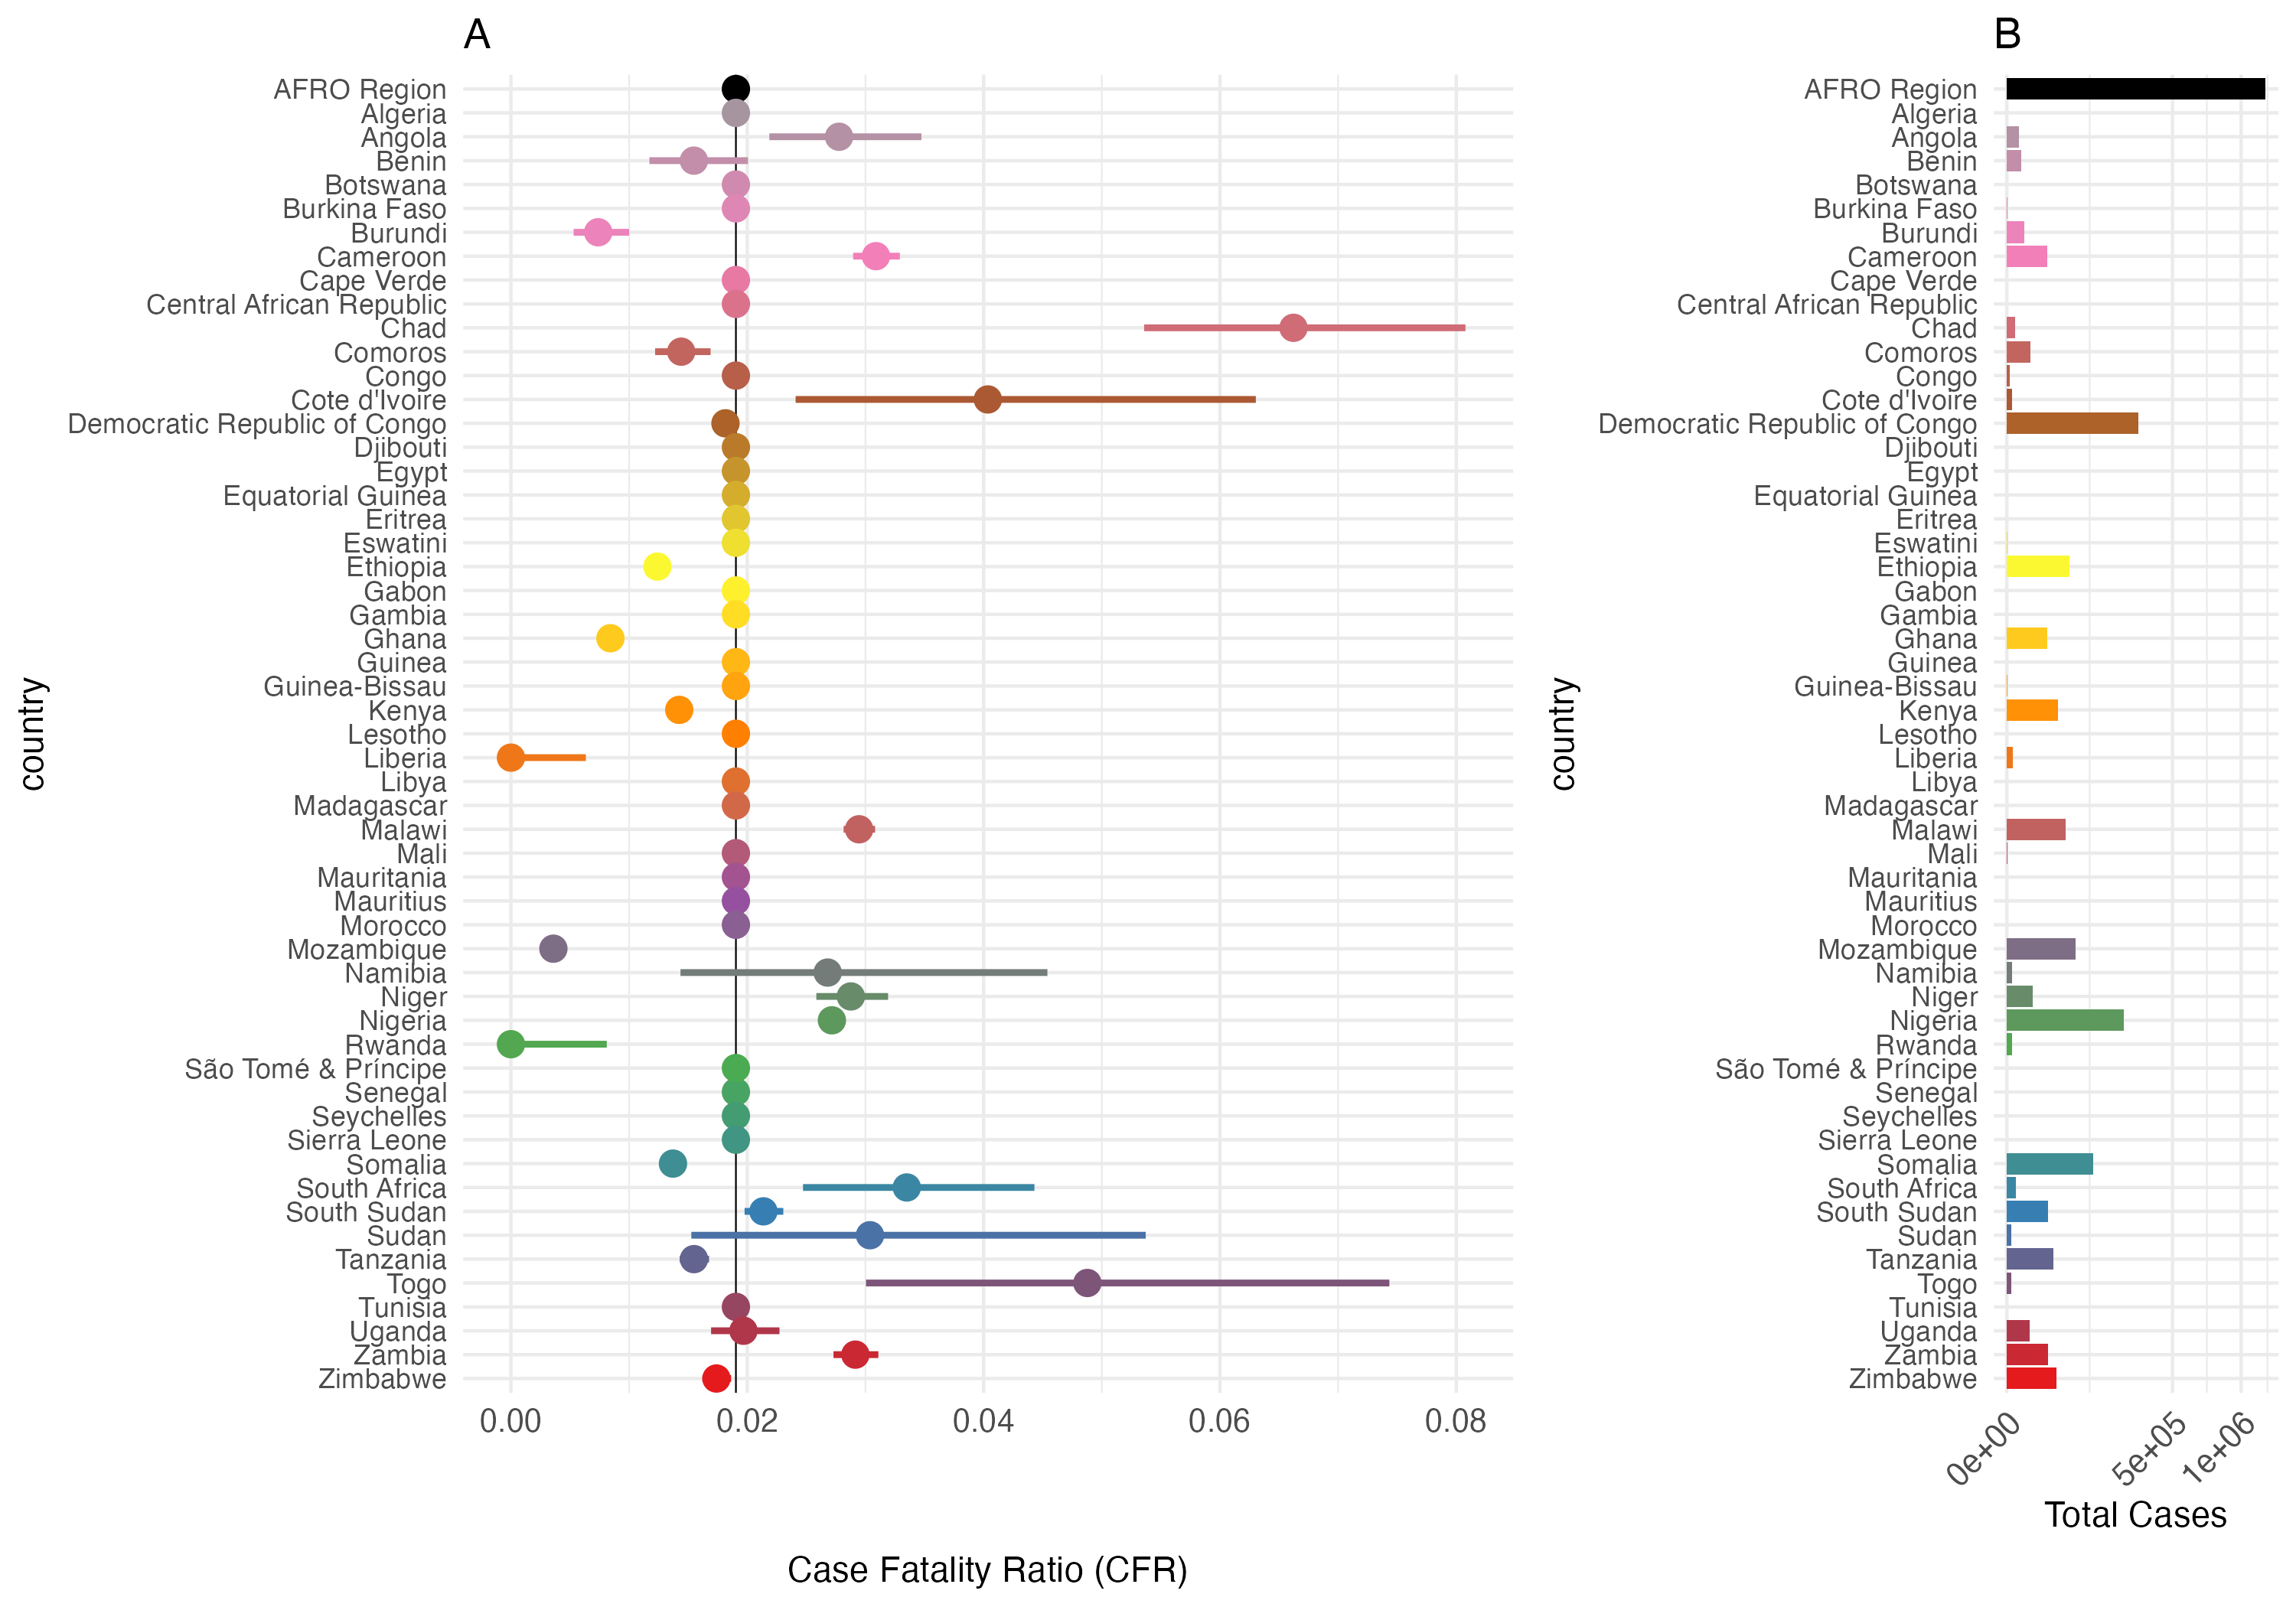
\includegraphics[width=1\linewidth]{figures/case_fatality_ratio_and_cases_total_by_country} 

}

\caption{Case Fatality Rate (CFR) and Total Cases by Country in the AFRO Region from 2014 to 2024. Panel A: Case Fatality Ratio (CFR) with 95\% confidence intervals. Panel B: total number of cholera cases. The AFRO Region is highlighted in black, all countries with less than 3/0.2 = 150 total reported cases are assigned the mean CFR for AFRO.}\label{fig:cfr-cases}
\end{figure}

\begin{figure}

{\centering 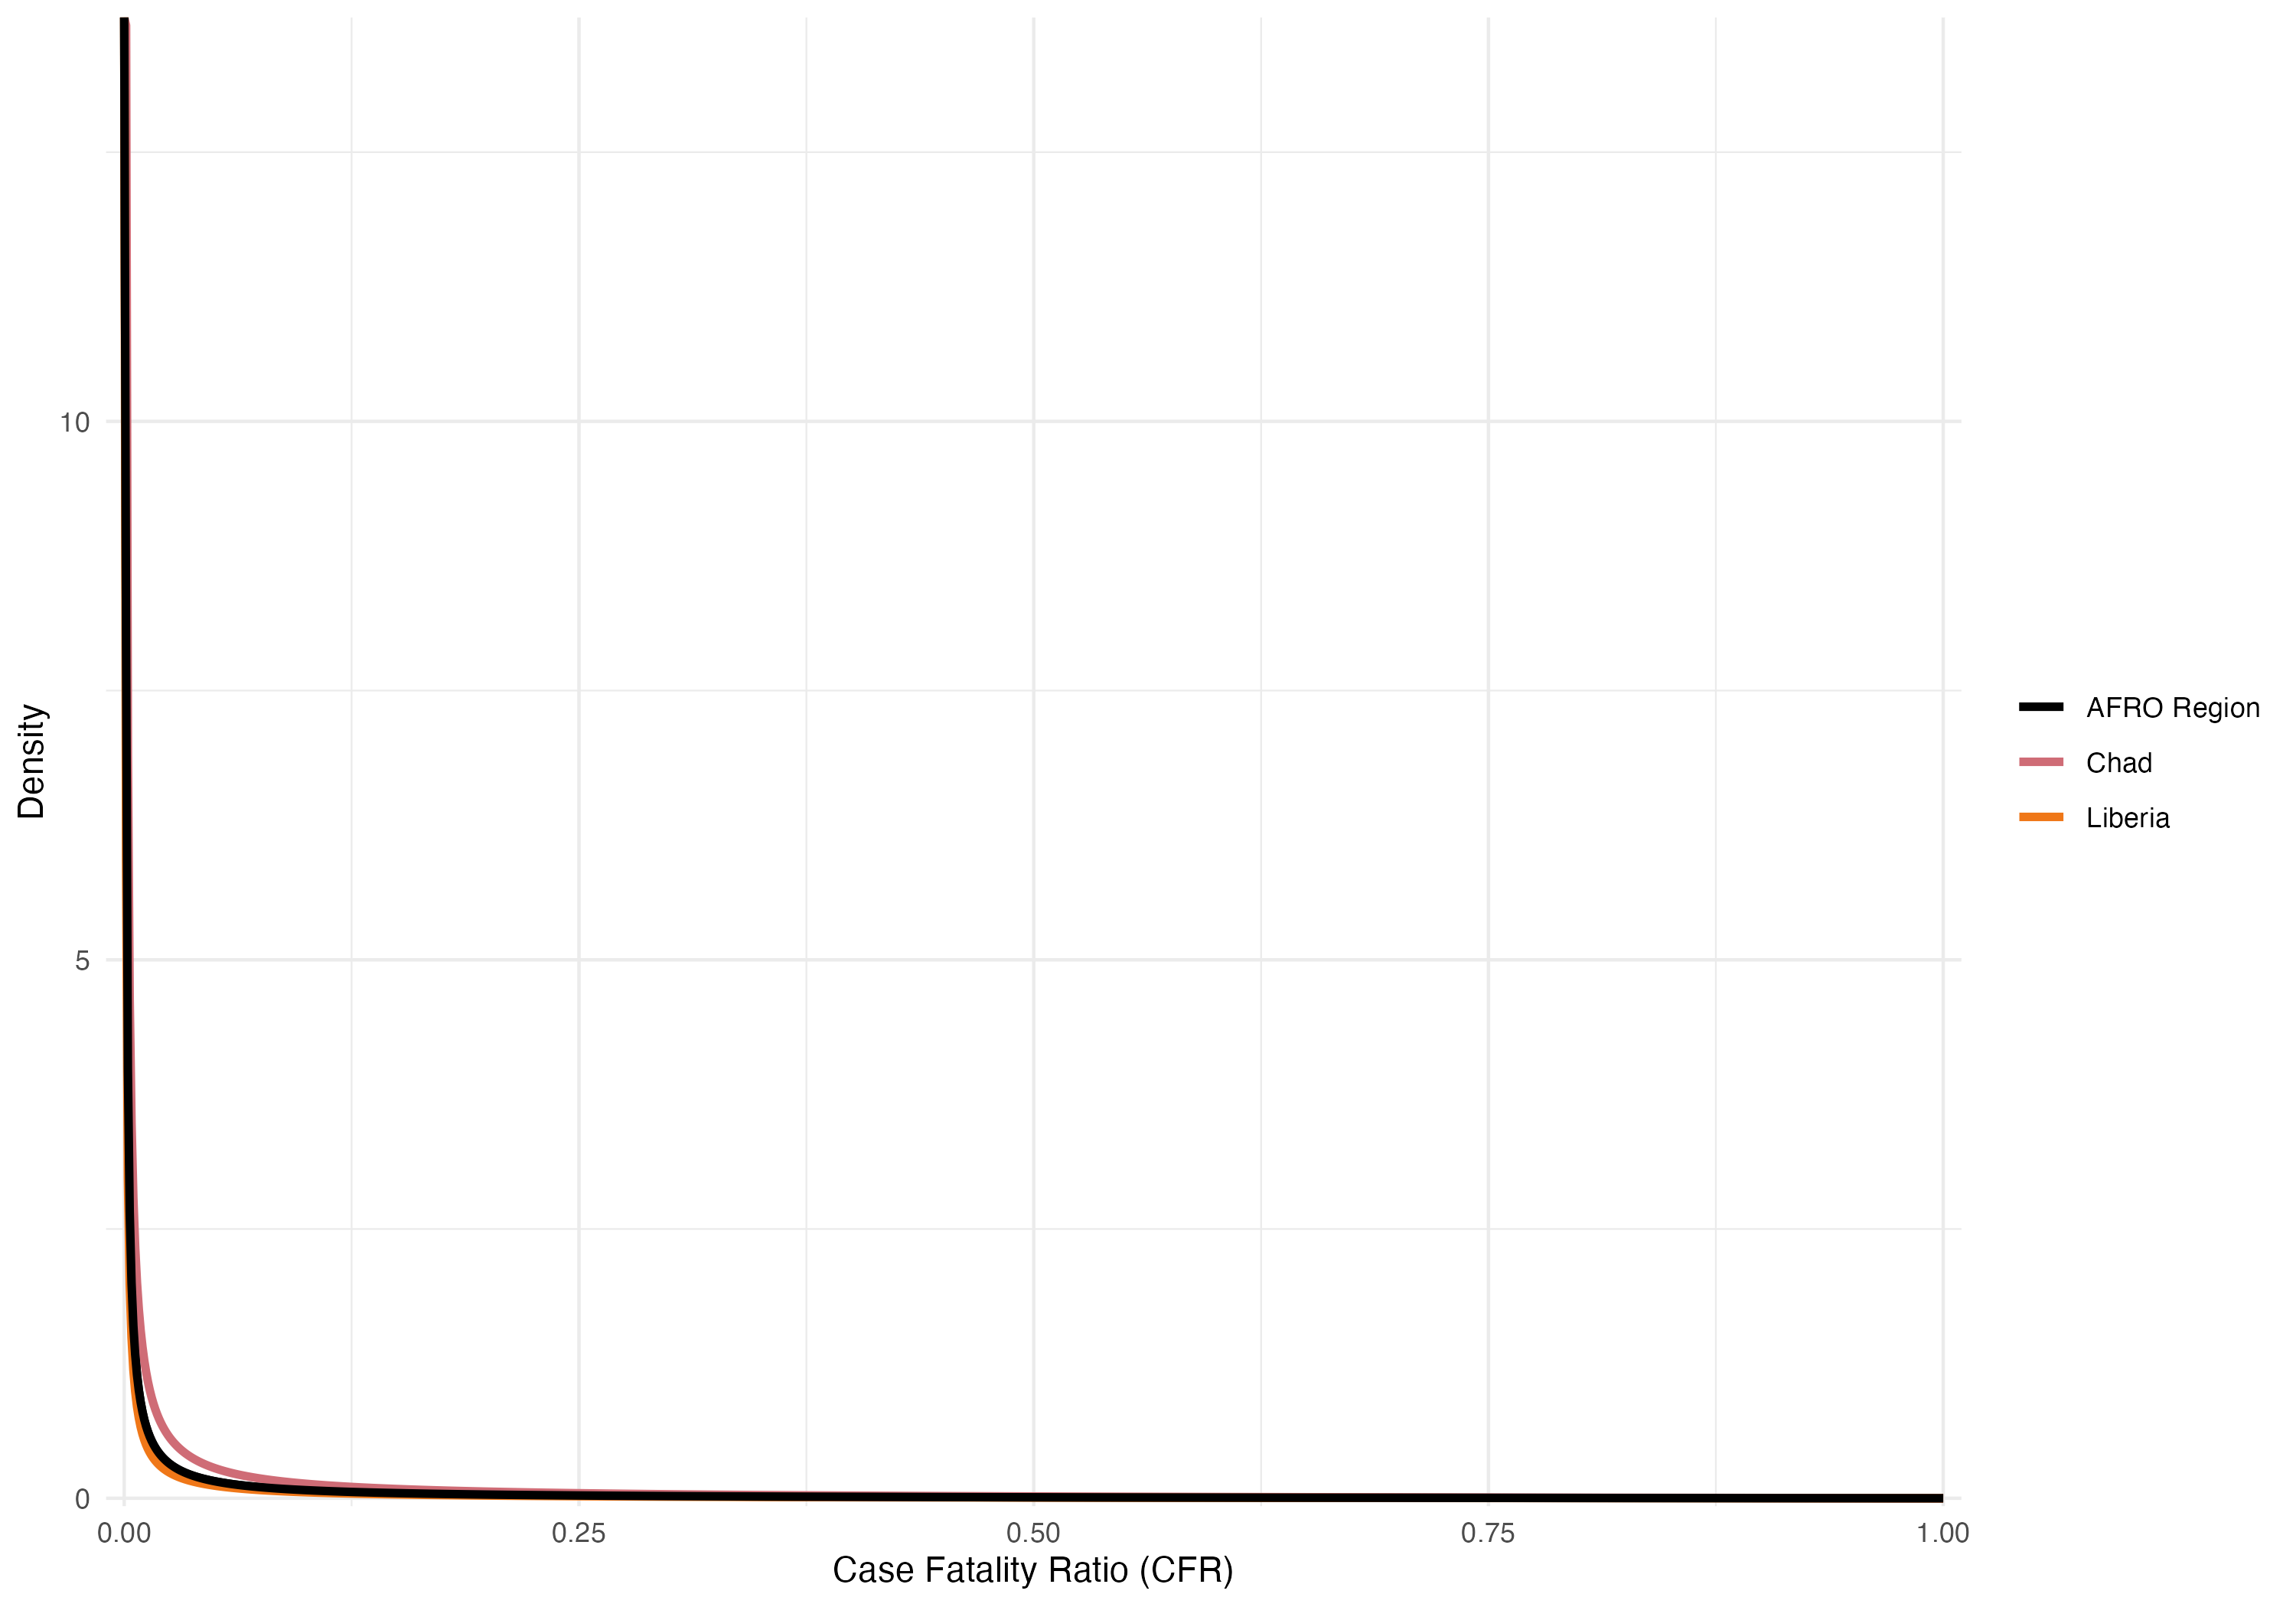
\includegraphics[width=0.95\linewidth]{figures/case_fatality_ratio_beta_distributions} 

}

\caption{Beta distributions of the overall Case Fatality Rate (CFR) from 2014 to 2024. Examples show the overall CFR for the AFRO region (2\%) in black, Congo with the highest CFR (7\%) in red, and South Sudan with the lowest CFR (0.1\%) in blue.}\label{fig:cfr-beta}
\end{figure}

\section{Demographics}\label{demographics-1}

The model includes basic demographic change by using reported birth and death rates for each of the \(j\) countries, \(b_j\) and \(d_j\) respectively. These rates are static and defined by the United Nations Department of Economic and Social Affairs Population Division \href{https://population.un.org/wpp/Download/Standard/CSV/}{World Population Prospects 2024}. Values for \(b_j\) and \(d_j\) are derived from crude rates and converted to birth rate per day and death rate per day (shown in Table \ref{tab:demographics}).

\begin{table}
\centering
\caption{\label{tab:demographics}Demographic for AFRO countries in 2023. Data include: total population as of January 1, 2023, daily birth rate, and daily death rate. Values are calculate from crude birth and death rates from UN World Population Prospects 2024.}
\centering
\begin{tabular}[t]{l|r|r|r}
\hline
Country & Population & Birth rate & Death rate\\
\hline
Algeria & 45831343 & 0.0000542 & 1.28e-05\\
\hline
Angola & 36186956 & 0.0001046 & 1.93e-05\\
\hline
Benin & 13934166 & 0.0000940 & 2.44e-05\\
\hline
Botswana & 2459937 & 0.0000683 & 1.58e-05\\
\hline
Burkina Faso & 22765636 & 0.0000877 & 2.21e-05\\
\hline
Burundi & 13503998 & 0.0000935 & 1.87e-05\\
\hline
Cameroon & 27997833 & 0.0000937 & 1.99e-05\\
\hline
Cape Verde & 521047 & 0.0000339 & 1.39e-05\\
\hline
Central African Republic & 5064592 & 0.0001292 & 2.63e-05\\
\hline
Chad & 18767684 & 0.0001196 & 3.11e-05\\
\hline
Comoros & 842267 & 0.0000793 & 1.99e-05\\
\hline
Congo & 6108142 & 0.0000849 & 1.74e-05\\
\hline
Côte d’Ivoire & 30783520 & 0.0000887 & 2.12e-05\\
\hline
Democratic Republic of Congo & 104063312 & 0.0001150 & 2.37e-05\\
\hline
Equatorial Guinea & 1825480 & 0.0000821 & 2.18e-05\\
\hline
Eritrea & 3438999 & 0.0000789 & 1.67e-05\\
\hline
Eswatini & 1224706 & 0.0000663 & 2.12e-05\\
\hline
Ethiopia & 127028360 & 0.0000886 & 1.65e-05\\
\hline
Gabon & 2457715 & 0.0000766 & 1.74e-05\\
\hline
Gambia & 2666786 & 0.0000843 & 1.74e-05\\
\hline
Ghana & 33467371 & 0.0000728 & 1.95e-05\\
\hline
Guinea & 14229395 & 0.0000939 & 2.53e-05\\
\hline
Guinea-Bissau & 2129290 & 0.0000832 & 1.95e-05\\
\hline
Kenya & 54793511 & 0.0000750 & 2.00e-05\\
\hline
Lesotho & 2298496 & 0.0000664 & 2.93e-05\\
\hline
Liberia & 5432670 & 0.0000858 & 2.24e-05\\
\hline
Madagascar & 30813475 & 0.0000890 & 2.09e-05\\
\hline
Malawi & 20832833 & 0.0000871 & 1.49e-05\\
\hline
Mali & 23415909 & 0.0001113 & 2.40e-05\\
\hline
Mauritania & 4948362 & 0.0000957 & 1.54e-05\\
\hline
Mauritius & 1274659 & 0.0000254 & 2.39e-05\\
\hline
Mozambique & 33140626 & 0.0001042 & 1.95e-05\\
\hline
Namibia & 2928037 & 0.0000718 & 1.71e-05\\
\hline
Niger & 25727295 & 0.0001167 & 2.47e-05\\
\hline
Nigeria & 225494749 & 0.0000912 & 3.25e-05\\
\hline
Rwanda & 13802596 & 0.0000785 & 1.64e-05\\
\hline
São Tomé \& Príncipe & 228558 & 0.0000780 & 1.54e-05\\
\hline
Senegal & 17867073 & 0.0000816 & 1.55e-05\\
\hline
Seychelles & 126694 & 0.0000377 & 2.27e-05\\
\hline
Sierra Leone & 8368119 & 0.0000848 & 2.30e-05\\
\hline
Somalia & 18031404 & 0.0001198 & 2.74e-05\\
\hline
South Africa & 62796883 & 0.0000518 & 2.55e-05\\
\hline
South Sudan & 11146895 & 0.0000807 & 2.71e-05\\
\hline
Tanzania & 65657004 & 0.0000979 & 1.61e-05\\
\hline
Togo & 9196283 & 0.0000863 & 2.13e-05\\
\hline
Uganda & 47981110 & 0.0000978 & 1.35e-05\\
\hline
Zambia & 20430382 & 0.0000919 & 1.45e-05\\
\hline
Zimbabwe & 16203259 & 0.0000840 & 2.10e-05\\
\hline
\end{tabular}
\end{table}

\section{The reproductive number}\label{the-reproductive-number}

The reproductive number is a common metric of epidemic growth that represents the average number of secondary cases generated by a primary case at a specific time during an epidemic. We track how \(R\) changes over time by estimating the instantaneous reproductive number \(R_t\) as described in \href{https://academic.oup.com/aje/article/178/9/1505/89262}{Cori et al 2013}. We track \(R_t\) across all metapopulations in the model to give \(R_{jt}\) using the following formula:

\begin{equation}
R_{jt} = \frac{I_{jt}}{\sum_{\Delta t=1}^{t} g(\Delta t) I_{j,t-\Delta t}}
\label{eq:R}
\end{equation}

Where \(I_{jt}\) is the number of new infections in destination \(j\) at time \(t\), and
\(g(\Delta t)\) represents the probability value from the generation time distribution of cholera. This is accomplished by using the weighed sum in the denominator which is highly influenced by the generation time distribution.

\subsection{The generation time distribution}\label{the-generation-time-distribution}

The generation time distribution gives the time between when an individual is infected and when they infect subsequent individuals. We parameterized this quantity using a Gamma distribution with a mean of 5 days:

\begin{equation}
g(\cdot) \sim \text{Gamma}(0.5, 0.1).
\label{eq:generation-time}
\end{equation}

Here, shape=0.5, rate=0.1, and the mean if given by shape/rate. Previous studies use a mean of 5 days (\href{https://www.ncbi.nlm.nih.gov/pmc/articles/PMC7060667/\#:~:text=The\%20serial\%20interval\%20for\%20cholera,routes\%20(45\%2C\%2046).}{Kahn et al 2020} and \href{https://www.ncbi.nlm.nih.gov/pmc/articles/PMC4880069/}{Azman 2016}), however a mean of 3, 5, 7, or 10 days may be admissible (\href{https://journals.plos.org/plosntds/article?id=10.1371/journal.pntd.0001901}{Azman 2012}).

\begin{figure}

{\centering 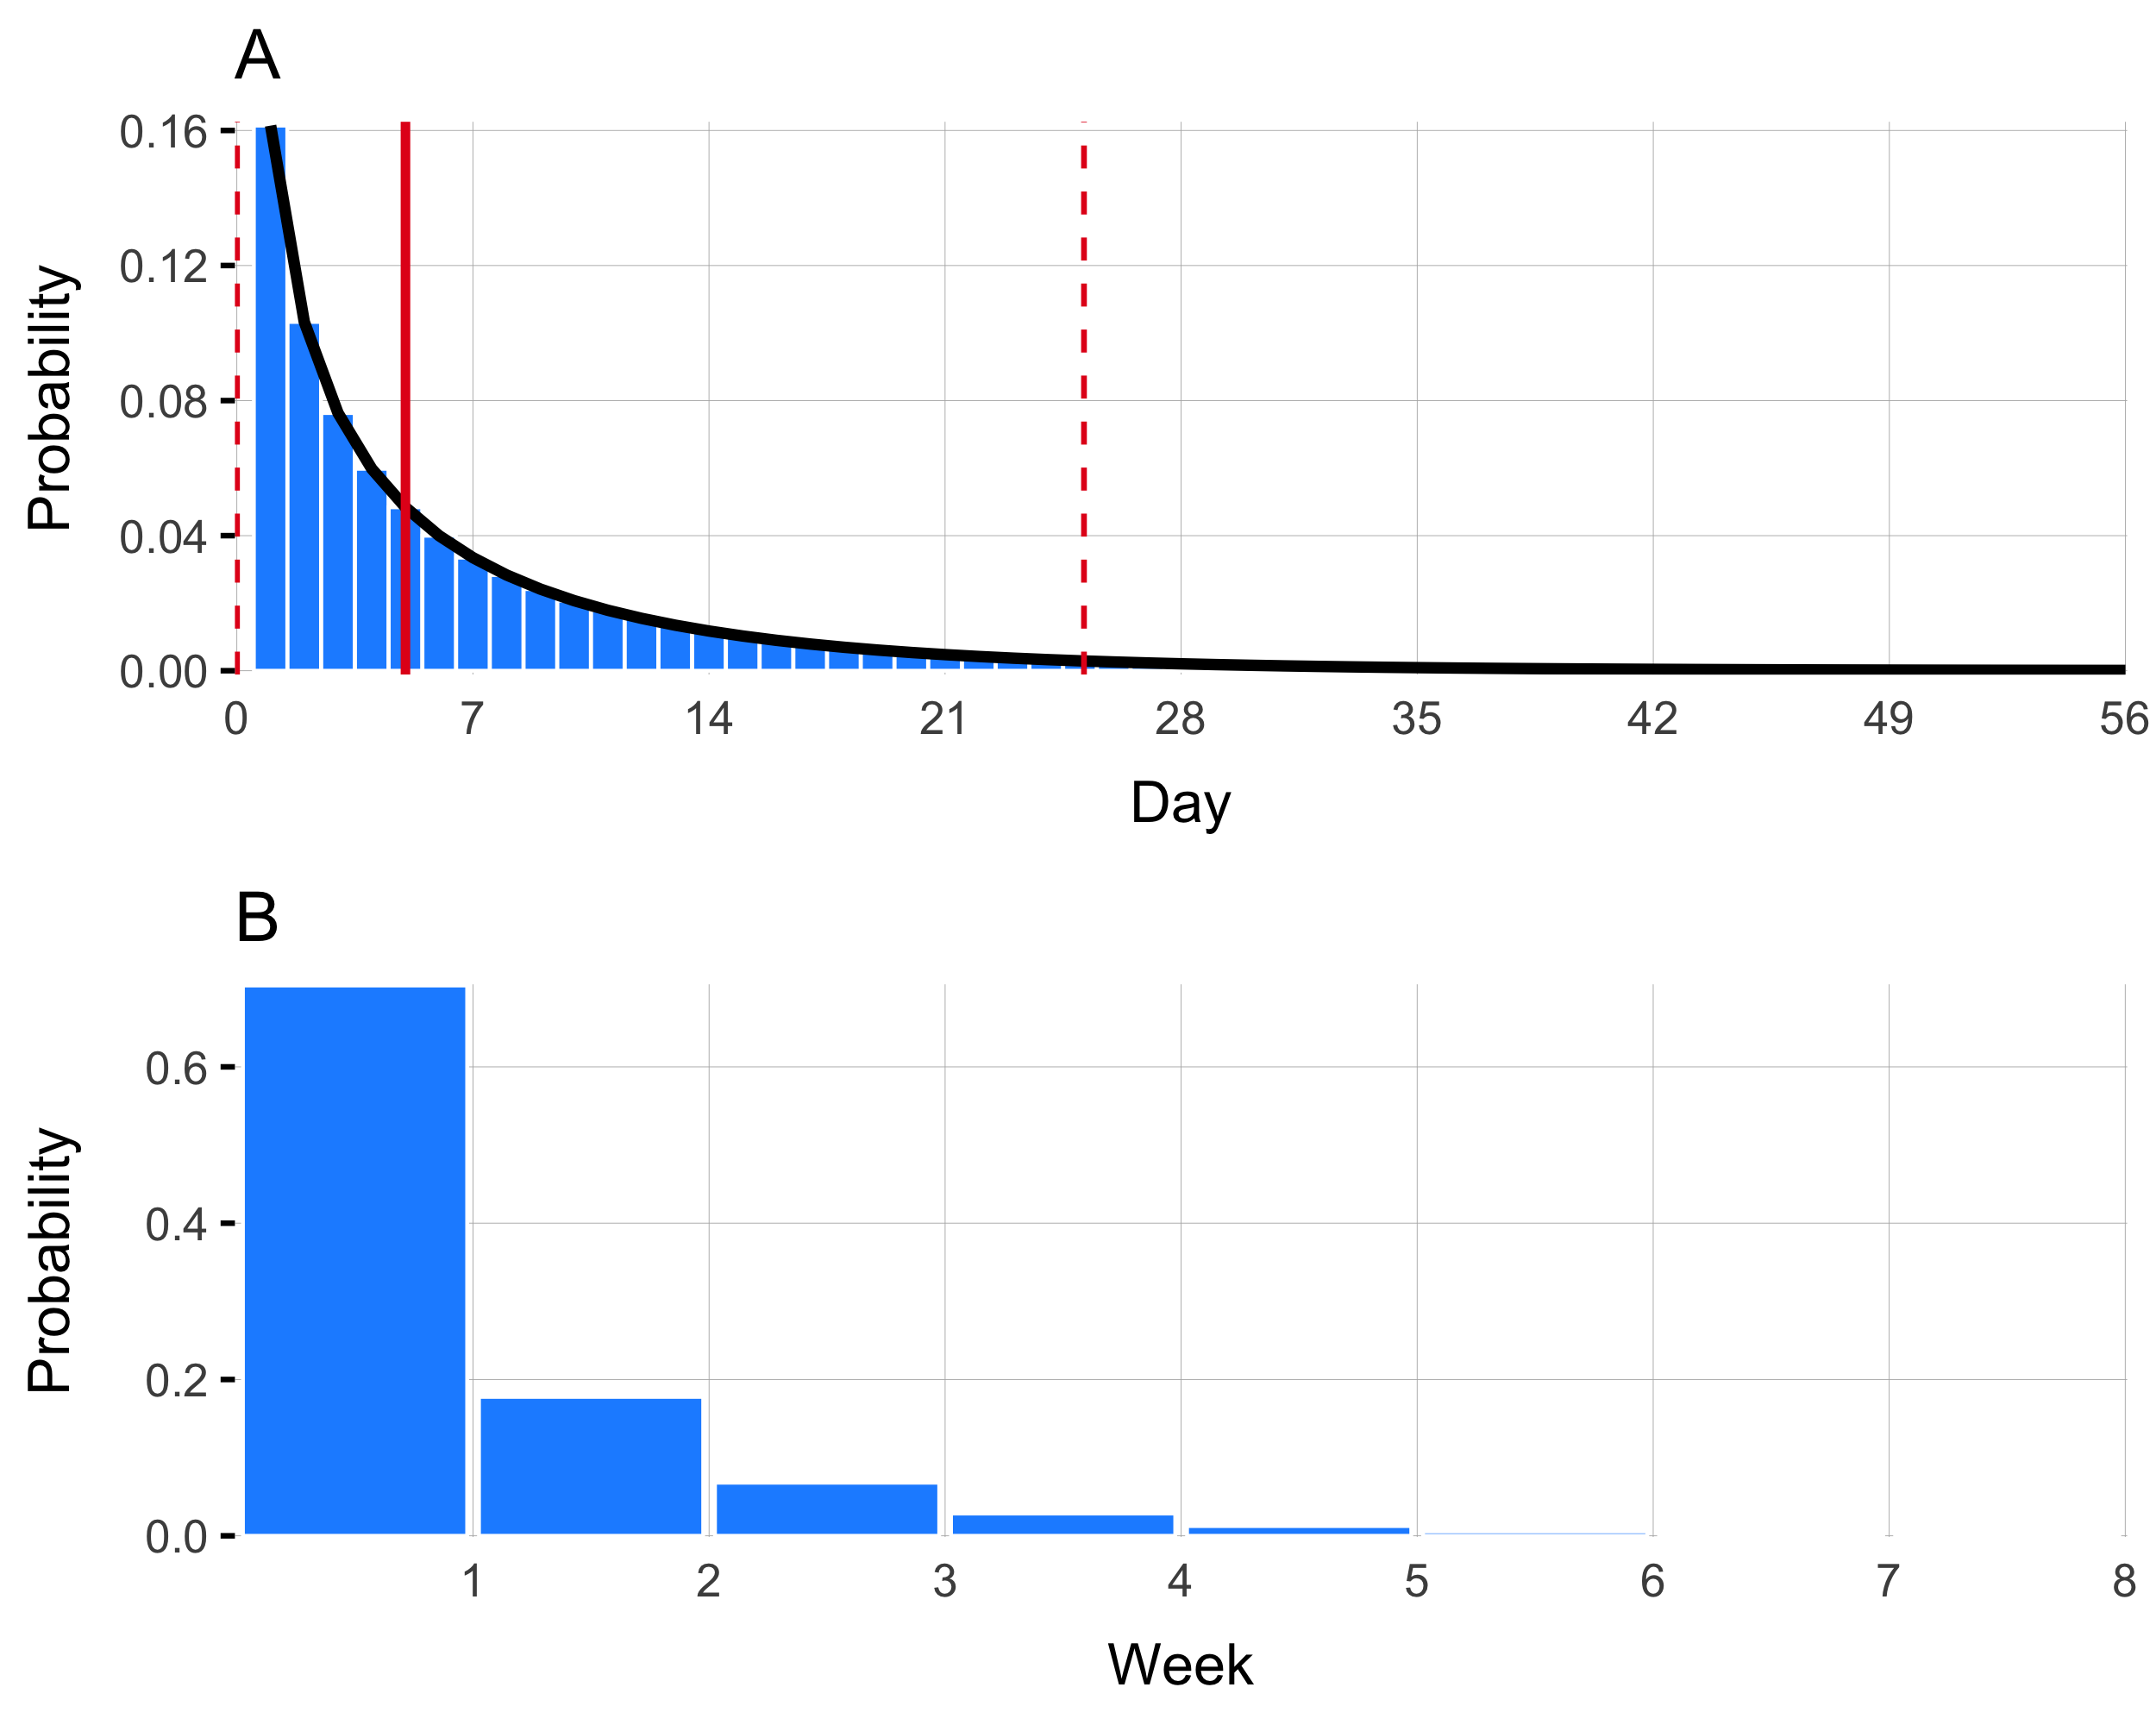
\includegraphics[width=0.95\linewidth]{figures/generation_time} 

}

\caption{This is generation time}\label{fig:generation}
\end{figure}

\begin{table}
\centering
\caption{\label{tab:unnamed-chunk-3}Generation Time in Weeks}
\centering
\begin{tabular}[t]{l|r|r}
\hline
Interval & Week & Probability\\
\hline
[0,7] & 1 & 0.704\\
\hline
(7,14] & 2 & 0.178\\
\hline
(14,21] & 3 & 0.068\\
\hline
(21,28] & 4 & 0.028\\
\hline
(28,35] & 5 & 0.012\\
\hline
(35,42] & 6 & 0.006\\
\hline
(42,49] & 7 & 0.003\\
\hline
(49,56] & 8 & 0.001\\
\hline
\end{tabular}
\end{table}

\section{Initial conditions}\label{initial-conditions}

Since this first version of the model will begin on Jan 2023 (to take advantage of available weekly data), the initial conditions surrounding population immunity must be estimated. To set these initial conditions, we use historical data to find the total number of reported cases for a location over the previous X years, multiply by \(1/\sigma\) to estimate total infections from those symptomatic cases that are reported, and then adjust based on waning immunity. We also sum the total number of vaccinations over the past X years and adjust for vaccine efficacy \(\phi\) and waning immunity from vaccination \(\omega\).

\begin{itemize}
\item
  total number infected? From reported cases\ldots{} back out symptomatic and asymptomatic
\item
  Total number immune due to natural infections in the past X years
\item
  total number immune due to past vaccinations in the X years
\end{itemize}

Use deconvolution based on immune decay estimated in vaccine section

\section{Model calibration}\label{model-calibration}

\begin{itemize}
\item
  The model will be calibrated using Latin hypercube sampling for hyper-parameters and model likelihoods fit to incidence and deaths.
\item
  An important challenge is flexibly fitting to data that are often missing or only available in aggregated forms.
\end{itemize}

{[}Fig: different spatial and temporal scales of available data{]}

\section{Caveats}\label{caveats}

\begin{itemize}
\tightlist
\item
  Simplest model to start. Easier for initial spatial structure but with minimum additional compartments to calibrate to available data (vaccination, cases, deaths).
\item
  Country level aggregations. First generation data is 2023/24\ldots{}
\item
  Assumes vaccinating susceptible only individuals.
\item
  For climate, summarizing for whole country.
\end{itemize}

\section{Table of parameters}\label{table-of-parameters}

\begin{table}

\caption{\label{tab:params}Descriptions of model parameters along with prior distributions and sources where applicable.}
\centering
\begin{tabular}[t]{l|l|l|l}
\hline
Parameter & Description & Distribution & Source\\
\hline
\$i\$ & Index \$i\$ represents the origin metapopulation. &  & \\
\hline
\$j\$ & Index \$j\$ represents the destination metapopulation. &  & \\
\hline
\$t\$ & Index \$t\$ is the time step which is one week (7 days). &  & \\
\hline
\$b\_j\$ & Birth rate of population \$j\$. &  & \\
\hline
\$d\_j\$ & Overall mortality rate of population \$j\$. &  & \\
\hline
\$N\_\{jt\}\$ & Total population size of destination \$j\$ at time \$t\$. &  & \\
\hline
\$S\_\{jt\}\$ & Number of susceptible individuals in destination \$j\$ at time \$t\$. &  & \\
\hline
\$V\_\{jt\}\$ & Number of effectively vaccinated individuals in destination \$j\$ at time \$t\$. &  & \\
\hline
\$I\_\{jt\}\$ & Number of infected individuals in destination \$j\$ at time \$t\$. &  & \\
\hline
\$W\_\{jt\}\$ & Total amount of V. cholerae in the environment in destination \$j\$ at time \$t\$. &  & \\
\hline
\$R\_\{jt\}\$ & Number of recovered (and therefore immune) individuals in destination \$j\$ at time \$t\$. &  & \\
\hline
\$\textbackslash{}Lambda\_\{j,t+1\}\$ & The force of infection due to human-to-human transmission in destination \$j\$ at time step \$t+1\$. &  & \\
\hline
\$\textbackslash{}Psi\_\{j,t+1\}\$ & The force of infection due to environment-to-human transmission in destination \$j\$ at time step \$t+1\$. &  & \\
\hline
\$\textbackslash{}phi\$ & The effectiveness of Oral Cholera Vaccine (OCV). &  & \\
\hline
\$\textbackslash{}nu\_\{jt\}\$ & The reported rate of vaccination with OCV in destination \$j\$ at time \$t\$. &  & \\
\hline
\$\textbackslash{}omega\$ & Rate of waning immunity of vaccinated individuals. &  & \\
\hline
\$\textbackslash{}varepsilon\$ & Rate of waning immunity of recovered individuals. &  & \\
\hline
\$\textbackslash{}gamma\$ & Recovery rate of infected individuals. &  & \\
\hline
\$\textbackslash{}mu\$ & Mortality rate due to infection with *V. cholerae*. &  & \\
\hline
\$\textbackslash{}sigma\$ & Proportion of *V. cholerae* infections that are symptomatic. &  & \\
\hline
\$\textbackslash{}rho\$ & The proportion of suspected cholera cases that are true infections. &  & \\
\hline
\$\textbackslash{}zeta\$ & Rate that infected individuals shed *V. cholerae* into the environment. & \$0.1\textbackslash{}mbox\{-\}10\$ & \\
\hline
\$\textbackslash{}delta\$ & The environmental suitability dependent decay rate of *V. cholerae* in the environment. &  & \\
\hline
\$\textbackslash{}delta\_\{\textbackslash{}text\{min\}\}\$ & The minimum decay rate of *V. cholerae* in the environment obtained when environmental suitability (\$\textbackslash{}psi\_\{jt\}\$) = 0. &  & \\
\hline
\$\textbackslash{}delta\_\{\textbackslash{}text\{max\}\}\$ & The maximum decay rate of *V. cholerae* in the environment obtained when environmental suitability  (\$\textbackslash{}psi\_\{jt\}\$) = 1. &  & \\
\hline
\$\textbackslash{}psi\_\{jt\}\$ & The climatically driven environmental suitability of *V. cholerae* in destination \$j\$ at time \$t\$. &  & \\
\hline
\$\textbackslash{}beta\_\{j0\}\textasciicircum{}\{\textbackslash{}text\{hum\}\}\$ & The baseline rate of human-to-human transmission in destination \$j\$. &  & \\
\hline
\$\textbackslash{}beta\_\{jt\}\textasciicircum{}\{\textbackslash{}text\{hum\}\}\$ & The seasonal rate of human-to-human transmission in destination \$j\$ at time \$t\$. &  & \\
\hline
\$\textbackslash{}beta\_\{j0\}\textasciicircum{}\{\textbackslash{}text\{env\}\}\$ & The baseline rate of environment-to-human transmission in destination \$j\$. &  & \\
\hline
\$\textbackslash{}beta\_\{jt\}\textasciicircum{}\{\textbackslash{}text\{env\}\}\$ & The rate of environment-to-human transmission in destination \$j\$ at time \$t\$. &  & \\
\hline
\$\textbackslash{}alpha\$ & The overall population mixing parameter. & 0.95 & [Glass et al 2003](https://www.sciencedirect.com/science/article/abs/pii/S0022519303000316)\\
\hline
\$\textbackslash{}tau\_i\$ & The probability that an individual departs origin \$i\$. &  & \\
\hline
\$\textbackslash{}pi\_\{ij\}\$ & The probability that an individual travels from origin \$i\$ to destination \$j\$ given that they have departed origin \$i\$. &  & \\
\hline
\$\textbackslash{}theta\_\{j\}\$ & The proportion of the population that have adequate Water, Sanitation and Hygiene (WASH). &  & \\
\hline
\$\textbackslash{}kappa\$ & The concentration (number of cells per mL) of *V. cholerae* required for a 50\% probability of infection. & \$10\textasciicircum{}5\textbackslash{}mbox\{-\}10\textasciicircum{}6\$ & [Fung 2014](https://www.ncbi.nlm.nih.gov/pmc/articles/PMC3926264/)\\
\hline
\end{tabular}
\end{table}

\section{References}\label{references}

\chapter{Model versions}\label{model-versions}

\begin{table}

\caption{\label{tab:unnamed-chunk-1}Current and future planned model versions with brief descriptions.}
\centering
\begin{tabular}[t]{l|l}
\hline
Version & Description\\
\hline
v0.1 & **Current:** Beta version of the model to establish mechanisms and links to data. Basic SIR dynamics with mobility, vaccination, environmental transmission, and an observation process.\\
\hline
v1.0 & **Future:** First implementation in LASER. Model definition is the same. Improvements to data sources and model adjustments to new data.\\
\hline
v2.0 & **Future:** Maximizing metapopulation approach. District level data and improvements to model fitting and hierarchical likelihoods. Likely in LASER, but could still have an R implementation at this point.\\
\hline
v3.0 & **Future:** Agent-based component with better immune dynamics.\\
\hline
\end{tabular}
\end{table}

\chapter{Scenarios}\label{scenarios}

A key aim of the MOSAIC model is to provide near-term forecasts of cholera transmission in Sub-Saharan Africa (SSA) using the most current data available. However, MOSAIC is not just a forecasting tool; it is a dynamic model designed to explore various scenarios that influence critical factors such as vaccination, environmental conditions, and Water, Sanitation, and Hygiene (WASH) interventions.

\section{Vaccination}\label{vaccination}

\subsection{Spatial and Temporal Strategies}\label{spatial-and-temporal-strategies}

Understanding the spatial and temporal distribution of cholera vaccination efforts is crucial for effective outbreak control. Key resources include:

\begin{itemize}
\tightlist
\item
  \textbf{Stockpile Status}: The availability of the oral cholera vaccine in emergency stockpiles can be tracked through UNICEF's \href{https://www.unicef.org/supply/documents/emergency-stockpile-availability-oral-cholera-vaccine}{Emergency Stockpile Availability}.
\item
  \textbf{WHO OCV Dashboard}: This dashboard (\href{https://app.powerbi.com/view?r=eyJrIjoiYmFmZTBmM2EtYWM3Mi00NWYwLTg3YjgtN2Q0MjM5ZmE1ZjFkIiwidCI6ImY2MTBjMGI3LWJkMjQtNGIzOS04MTBiLTNkYzI4MGFmYjU5MCIsImMiOjh9}{link}) provides insights into the deployment of oral cholera vaccines (OCV) across different regions.
\end{itemize}

\subsection{Reactive Vaccination}\label{reactive-vaccination}

The timing and logistics of reactive vaccination campaigns are critical for controlling ongoing outbreaks. Relevant resources include:

\begin{itemize}
\tightlist
\item
  \textbf{WHO Recommended Timing}: Guidelines and recommendations for the timing of reactive OCV campaigns are available from the WHO (\href{https://www.who.int/groups/icg/cholera/stockpiles}{link}).
\item
  \textbf{Requests and Delay Time Distributions}: Information on vaccine request processes and the distribution of delays in vaccine deployment can be accessed through the GTFCC OCV Dashboard (\href{https://apps.epicentre-msf.org/public/app/gtfcc}{link}).
\end{itemize}

\section{Impacts of Climate Change}\label{impacts-of-climate-change-1}

\subsection{Severe Weather Events}\label{severe-weather-events}

Projections of climate shocks, including the frequency and severity of cyclones and floods, are essential for modeling the future impacts of climate change on cholera transmission. Key references include:

\begin{itemize}
\tightlist
\item
  \textbf{Chen and Chavas 2020}: A study on cyclone season dynamics under climate change scenarios (\href{https://journals.ametsoc.org/view/journals/atsc/77/8/jasD190320.xml}{link}).
\item
  \textbf{Sparks and Toumi 2024}: Research on projected flood frequencies due to climate change (\href{https://www.nature.com/articles/s41597-024-03250-y}{link}).
\item
  \textbf{Switzer et al.~2023}: An analysis of climate shock impacts on cholera outbreaks (\href{https://www.nature.com/articles/s43247-023-00844-z}{link}).
\end{itemize}

\subsection{Long-Term Trends}\label{long-term-trends}

Long-term trends in weather variables under various climate change scenarios can be explored using the following resource:

\begin{itemize}
\tightlist
\item
  \textbf{Weather Variables Under Climate Change}: The OpenMeteo Climate API provides access to projected weather data under different climate change scenarios (\href{https://open-meteo.com/en/docs/climate-api}{link}).
\end{itemize}

\chapter{Usage}\label{usage}

The open-source code used to run MOSAIC is currently under development and will be presented here in the future.

\chapter{News}\label{news}

\section*{November 25, 2024 --- The MOSAIC framework presented at ASMTH 2024}\label{november-25-2024-the-mosaic-framework-presented-at-asmth-2024}
\addcontentsline{toc}{section}{November 25, 2024 --- The MOSAIC framework presented at ASMTH 2024}

John Giles presented the MOSAIC modeling framework in a talk entitled ``\emph{Cholera modeling capacity at IDM:
leveraging diverse data streams for scenarios and forecasting}'' at the American Society of Tropical Medicine and Hygiene (ASTMH) on November 14, 2024 as part the symposium entitled ``\emph{Infectious Disease Surveillance and Modeling in LMIC's: From Data Collection to Forecasting}''.

\chapter{References}\label{references-1}

  \bibliography{references.bib}

\end{document}
